% For printing in a4
\documentclass[a4,10pt,twoside,openright,italian,english]{book}% twoside!

% For printing with the A5 format
%\documentclass[10pt,twoside,openright,english,italian]{book}% twoside!

% Set paper size
\usepackage[twoside=true]{geometry}

%For printing with the weird format
%\geometry{
%	paperwidth=17cm,
%	paperheight=24cm,
%	margin=2cm,
%	top=2.3cm,
%	bindingoffset=0.4cm
%}
% For printing in a4
\geometry{a4paper,
  margin=3cm,
  top=3.8cm,
  bindingoffset=0.4cm
}

%Uncomment this for final prints: this just enables printing on a4 paper
\usepackage[cam,center,a4,pdflatex,axes]{crop}

\usepackage{phdthesis}

%\usepackage{fancyhdr}
\usepackage{color}
\usepackage{array}
\usepackage{mdwmath}
\usepackage{mdwtab}
\usepackage{amsmath,amssymb}
%\usepackage{cite}
\usepackage[numbers]{natbib}

%\usepackage{graphicx}
\usepackage{listings}
\usepackage{subcaption}
\usepackage{booktabs}
\usepackage{latexsym}
%\usepackage{color}
\usepackage{url}
\usepackage{bnf}
\usepackage{cleveref} % adds "Figure" / "Section" words to cites
% \crefname{subsection}{subsection}{subsections}
\usepackage{rotating}
\usepackage{multirow}
\usepackage{phdtitle}
\usepackage{paralist}
\usepackage{bibentry}
%\usepackage[algochapter]{algorithm2e}
%\usepackage[bookmarks=true,
%pdftex=false,
%bookmarksopen=true,hidelinks]{hyperref}
%\usepackage[toc,acronym]{glossaries}
\usepackage{lscape}
\usepackage{algorithmic}
\usepackage{algorithm}
\usepackage{longtable}
\usepackage{tabularx}
\usepackage[T1]{fontenc}
%\usepackage[latin1]{inputenc}
\usepackage[utf8]{inputenc}
%\usepackage{fontspec}
%\setmainfont{Calibri}
%% \hyphenation{} is used to force the
\hyphenation{}

\usepackage{eurosym}
\usepackage{siunitx}
\sisetup{detect-weight=true, detect-family=true}
\usepackage{xfrac}

\newtheorem{Definition}{Definition}[section]
\DeclareMathOperator*{\argmin}{arg\,min}

\lstset{tabsize=2,basicstyle=\footnotesize,breaklines=true}

\usepackage[italian,main=english]{babel}
\usepackage{ulem}
\normalem

\hypersetup{pdftitle={Title}, pdfauthor={Author}}

\nobibliography*

\department {Dottorato di ricerca in Ingegneria dell'Informazione}

% Please fulfil the followed fields with your data
\author{Fabio Carrara}
\title{Deep Learning for Image Classification and Retrieval: Opportunities and Limitations}
\tutor{Tutor Name}
\supervisor{Coordinator Name}
\titleimage{img/unipi.png} %please not change
\phdyear{Year}
\phdmonth{Month}
\phdcycle{Cycle XXXI}

%%%%%%%%%%%%%%%%%%%%%%%%%%%%%%%%%%%%%%
% Let's Start The Real Document
%%%%%%%%%%%%%%%%%%%%%%%%%%%%%%%%%%%%%%
\newglossaryentry{matrix_channel}
{       name={$H^*$},
        description={Conjugate operation}
}
\newglossaryentry{trasp_x}
{       name={$[ x ]^{\rm T}$},
        description={transpose operator}
}
\newglossaryentry{vec_x}
{       name={\textbf{x}},
        description={vectors are in bold}
}
\newglossaryentry{floor_funct}
{       name={$\left\lfloor x \right\rfloor$},
        description={round to the lower integer of $x$}
}

% Deep Learning
\newacronym{ml}{ML}{Machine Learning}
\newacronym{dl}{DL}{Deep Learning}
\newacronym{dnn}{DNN}{Deep Neural Network}
\newacronym{ffnn}{FFNN}{Feed-Forward Neural Network}
\newacronym{rnn}{RNN}{Recurrent Neural Network}
\newacronym{mlp}{MLP}{Multilayer Perceptron}
\newacronym{cnn}{CNN}{Convolutional Neural Network}
\newacronym{dcnn}{DCNN}{Deep Convolutional Neural Network}
\newacronym{lstm}{LSTM}{Long Short-term Memory}
\newacronym{sgd}{SGD}{Stochastic Gradient Descent}
\newacronym{adam}{Adam}{Adaptive Moment Estimation}
\newacronym{relu}{ReLU}{Rectified Linear Unit}
\newacronym{resnet}{ResNet}{Residual Network}
\newacronym{senet}{SENet}{Squeeze-and-Excitation Network}
\newacronym{bn}{BN}{Batch Normalization}
\newacronym{rmac}{R-MAC}{Regional Maximum Activation of Convolutions}

% Metrics
\newacronym{tpr}{TPR}{True Positive Rate}
\newacronym{tnr}{TNR}{True Negative Rate}
\newacronym{fpr}{FPR}{False Positive Rate}
\newacronym{fnr}{FNR}{False Negative Rate}
\newacronym{auc}{AUC}{Area Under the Curve}
\newacronym{roc}{ROC}{Receiver Operation Characteristics}
\newacronym{eer}{EER}{Equal Error Rate}
\newacronym{ap}{AP}{Average Precision}
\newacronym{map}{mAP}{mean Average Precision}
\newacronym{dcg}{DCG}{Discounted Cumulative Gain}
\newacronym{ndcg}{NDCG}{Normalized Discounted Cumulative Gain}
\newacronym{r@k}{R@K}{Recall at K}
\newacronym{medR}{medR}{Median Rank}
\newacronym{mrr}{MRR}{Mean Reciprocal Rank}

% CBIR
\newacronym{cbir}{CBIR}{Content-based Image Retrieval}
\newacronym{pca}{PCA}{Principal Component Analysis}

% Datasets
\newacronym{ilsvrc}{ILSVRC}{ImageNet Large Scale Visual Recognition Challenge}
\newacronym{coco}{COCO}{Common Objects in Context} % TODO check COCO acronym
\newacronym{t4sa}{T4SA}{Twitter for Sentiment Analysis}

% Others
\newacronym{gpu}{GPU}{Graphical Processing Unit}
\newacronym{lbp}{LBP}{Local Binary Patterns}
\newacronym{lpq}{LPQ}{Local Phase Quantization} % CHECK
\newacronym{str}{STR}{Surrogate Text Representation}
\newacronym{svm}{SVM}{Support Vector Machine}

\newacronym{vgg}{VGG}{Visual Geometry Group}



\makeglossaries

\begin{document}
\selectlanguage{english}

\maketitle

\pagestyle{empty}

\cleardoublepage
\newpage

%%%%%%%%%%%%%%%%%%%%%%%%%%%%%%%%%%%%%%
% Dedication - For removing dedication, please comment or delete the code inside \thispagestyle{empty}
%%%%%%%%%%%%%%%%%%%%%%%%%%%%%%%%%%%%%%
\thispagestyle{empty}
    \null\vspace{\stretch {1}}
        \begin{flushright}
                This thesis is dedicated to....
        \end{flushright}
\vspace{\stretch{2}}\null

\cleardoublepage
\newpage

\pagestyle{empty}
%% change numbering into Roman numbers for the introductory part
%\setcounter{page}{1}
%\pagenumbering{Roman}

%%%%%%%%%%%%%%%%%%%%%%%%%%%%%%%%%%%%%%
% Quotes - For removing quotes, please comment or delete the code inside \thispagestyle{empty}
%%%%%%%%%%%%%%%%%%%%%%%%%%%%%%%%%%%%%%
\thispagestyle{empty}
    \null\vspace{\stretch {1}}
        \begin{flushright}
                "A few first rate research papers are preferable to a large number \\
                that are poorly conceived or half-finished.\\
                The latter are no credit to their writers and \\
                a waste of time to their readers"\\
                Claude Shannon
                %IRE Transactions on Information Theory (1956), volume 2, issue 1, page 3. Shannon, Claude E. (March 1956), The Bandwagon, 2, doi:10.1109/TIT.1956.1056774.
        \end{flushright}
\vspace{\stretch{2}}\null

\cleardoublepage
\newpage

\pagestyle{empty}
%% change numbering into Roman numbers for the introductory part
\setcounter{page}{1}
\pagenumbering{Roman}

%%%%%%%%%%%%%%%%%%%%%%%%%%%%%%%%%%%%%%
% Acknowledgement
%%%%%%%%%%%%%%%%%%%%%%%%%%%%%%%%%%%%%%
\chapter*{Acknowledgements}
\lettrine{A}{cknowledgements} goes here.

\selectlanguage{italian}
%\chapter*{Ringraziamenti}
%\lettrine{R}{ingraziamenti}
% English-only Acknowledgements
\selectlanguage{english}

\cleardoublepage
\newpage

\pagestyle{fancy}
% change numbering into Roman numbers for the introductory part

%%%%%%%%%%%%%%%%%%%%%%%%%%%%%%%%%%%%%%
% Summary
%%%%%%%%%%%%%%%%%%%%%%%%%%%%%%%%%%%%%%
\selectlanguage{english}
\chapter*{Summary}
\lettrine{T}{he} large diffusion of cheap cameras and smartphones led to an exponential daily production of digital visual data, such as images and videos.
In this context, most of the produced data lack manually assigned metadata needed for their manageability in large-scale scenarios, thus shifting the attention to the automatic understanding of the visual content.
Recent developments in Computer Vision and Artificial Intelligence empowered machines with high-level vision perception enabling the automatic extraction of high-quality information from raw visual data.
Specifically, \acrfullpl{cnn} provided a way to automatically learn effective representations of images and other visual data showing impressive results in vision-based tasks, such as image recognition and retrieval.

In this thesis, we investigated and enhanced the usability of \acrshortpl{cnn} for visual data management.
First, we identify three main limitations encountered in the adoption of \acrshortpl{cnn} and propose general solutions that we experimentally evaluated in the context of image classification.
We proposed miniaturized architectures to decrease the usually high computational cost of \acrshortpl{cnn} and enable edge inference in low-powered embedded devices.
%We evaluated our proposal in a practical distributed application, i.e., visual parking lot occupancy detection, extensively comparing the reduced models to state-of-the-art methods and architectures.
We tackled the problem of manually building huge training sets for models by proposing an automatic pipeline for training classifiers based on cross-media learning and Web-scraped weakly-labeled data.
We analyzed the robustness of \acrshortpl{cnn} representations to out-of-distribution data, specifically the vulnerability to adversarial examples, and proposed a detection method to discard spurious classifications provided by the model.
%
Secondly, we focused on the integration of \acrshort{cnn}-based \acrfull{cbir} in the most commonly adopted search paradigm, that is, textual search.
We investigated solutions to bridge the gap between image search and highly-developed textual search technologies by reusing both the front-end (text-based queries) and the back-end (distributed and scalable inverted indexes). % in \acrshort{cbir} scenarios.
We proposed a cross-modal image retrieval approach which enables textual-based image search on unlabeled collections by learning a mapping from textual to high-level visual representations.
Finally, we formalized, improved, and proposed novel surrogate text representations, i.e., text transcriptions of visual representations that can be indexed and retrieved by available textual search engines enabling \acrshort{cbir} without specialized indexes.

\selectlanguage{english}

%%%%%%%%%%%%%%%%%%%%%%%%%%%%%%%%%%%%%%
% Italian Summary
%%%%%%%%%%%%%%%%%%%%%%%%%%%%%%%%%%%%%%

%There must be an Italian version of the summary
\selectlanguage{italian}
\chapter*{Sommario}
\lettrine{L'}{} enorme diffusione di fotocamere e smartphone a prezzi economici ha portato a una produzione esponenziale giornaliera di dati visivi digitali, come immagini e video.
La maggior parte dei dati prodotti non è accompagnata dai metadati, come descrizioni, tags, o altri dati manualmente assegnati, che sono necessari per la loro gestione automatica su larga scala.
L'attenzione della ricerca si è quindi spostata sulla comprensione automatica del contenuto visivo di tali dati.
I recenti sviluppi dell'Intelligenza Artificiale applicata alla Computer Vision hanno reso possibile l'estrazione automatica di informazioni di alta qualità direttamente da dati visivi grezzi (pixel).
In particolare, modelli neurali come le reti neurali convoluzionali hanno fornito un modo per apprendere automaticamente delle rappresentazioni numeriche efficaci per immagini e altri dati visivi che hanno ottenuto risultati impressionanti in task visivi come il riconoscimento di immagini.

In questa tesi, è stata studiata e migliorata l'usabilità delle reti neurali convoluzionali per la gestione dei dati visivi su larga scala.
Nella prima parte, sono state identificate tre limitazioni principali solitamente incontrate nell'utilizzo delle reti convoluzionali e sono state proposte delle soluzioni generali che abbiamo valutato sperimentalmente nel contesto della classificazione di immagini.
Sono state proposte architetture miniaturizzate per ridurre il costo computazionale solitamente elevato di questo tipo di reti e consentire quindi il loro utilizzo anche a bordo di dispositivi embedded a bassa potenza.
% Abbiamo valutato la nostra proposta in un'applicazione pratica e distribuita, ovvero la rilevazione di occupazione del parcheggio visivo, confrontando ampiamente i modelli ridotti con i metodi e le architetture più avanzati.
È stato affrontato il problema della creazione di training set per i modelli, che richiederebbero un notevole sforzo manuale, proponendo una pipeline automatica per allenare reti basata sul cross-media learning e su dati imprecisi provenienti dal Web.
È stata analizzata la robustezza delle rappresentazioni estratte dalle reti convoluzionali per dati fuori dalla distribuzione di train, con enfasi particolare sulla vulnerabilità delle reti agli attacchi avversari (adversarial examples), proponendo un metodo di rilevamento per scartare le classificazioni spurie fornite dal modello.
%
In secondo luogo, ci siamo concentrati sull'integrazione della ricerca per immagini, basata su rappresentazioni estratte da reti convoluzionali, col paradigma di ricerca più comunemente adottato, cioè la ricerca testuale.
In questo contesto, abbiamo studiato delle soluzioni per colmare il divario tra l'attuale stato dell'arte nella ricerca di immagini e le più mature tecnologie di ricerca testuale.
In particolare, sono state integrate soluzioni per la ricerca di immagini basata sul contenuto sia con il front-end (query testuali) che con il back-end (indici invertiti distribuiti e scalabili per documenti testuali).
Nel primo caso, è stato proposto un approccio di recupero di immagini cross-modale che consente la ricerca tramite descrizione testuale di immagini in collezioni non etichettate tramite l'apprendimento di una funzione di mapping delle rappresentazioni testuali in quelle visive.
Nel secondo caso, sono state formalizzate, migliorate e proposte nuove rappresentazioni testuali surrogate per immagini, che consistono in una trasformazione delle rappresentazioni visive in testo surrogato che può essere indicizzato e recuperato dai motori di ricerca testuali attualmente disponibili, abilitando applicazioni di recupero di immagini senza il bisogno di indici specializzati.

\selectlanguage{english}

%%%%%%%%%%%%%%%%%%%%%%%%%%%%%%%%%%%%%%
% Publications
%%%%%%%%%%%%%%%%%%%%%%%%%%%%%%%%%%%%%%

%List of publications of the PhD candidate
\selectlanguage{english}
\chapter*{List of publications}

% for citing your paper, take directly APA format from Google scholar
% \item Surname, N., Surname, N. and Surname, N. (Year,Month). Title of the paper or journal. \emph{Place of publication}. (Vol. 123, pp. 456). EditorName.

\section*{International Journals}
\begin{enumerate}
    \item Amato, G., Carrara, F., Falchi, F., Gennaro, C., Meghini, C., and Vairo, C. (2017, April). Deep learning for decentralized parking lot occupancy detection. \emph{Expert Systems with Applications}. (Vol. 72, pp. 327-334). Pergamon.
    \item Carrara, F., Esuli, A., Fagni, T., Falchi, F., and Fernández, A. M. (2018, June). Picture it in your mind: Generating high level visual representations from textual descriptions. \emph{Information Retrieval Journal}. (Vol. 21, pp. 208-229). Springer.
    % manca mese, volume e pagine
    \item Carrara, F., Falchi, F., Caldelli, R., Amato, G., and Becarelli, R. (2018). Adversarial image detection in deep neural networks. \emph{Multimedia Tools and Applications}. (pp. 1-21). Springer.

\end{enumerate}

\section*{International Conferences/Workshops with Peer Review}
\begin{enumerate}
    \item Amato, G., Carrara, F., Falchi, F., Gennaro, C., and Vairo, C. (2016, June). Car parking occupancy detection using smart camera networks and deep learning. In \emph{2016 IEEE Symposium on Computers and Communication (ISCC)}. (pp. 1212-1217). IEEE.
    \item Carrara, F., Falchi, F., Caldelli, R., Amato, G., Fumarola, R., and Becarelli, R. (2017, June). Detecting adversarial example attacks to deep neural networks. In \emph{Proceedings of the 15th International Workshop on Content-Based Multimedia Indexing (CBMI)}. (p. 38). ACM.
    \item Amato, G., Carrara, F., Falchi, F., and Gennaro, C. (2017, June). Efficient Indexing of Regional Maximum Activations of Convolutions using Full-Text Search Engines. In \emph{Proceedings of the 2017 ACM on International Conference on Multimedia Retrieval (ICMR)}. (pp. 420-423). ACM.
    \item Vadicamo, L., Carrara, F., Cimino, A., Cresci, S., Dell’Orletta, F., Falchi, F., and Tesconi, M. (2017, October). Cross-Media Learning for Image Sentiment Analysis in the Wild. In \emph{2017 IEEE International Conference on Computer Vision (ICCV) Workshops}. (pp. 308-317).
    \item Amato, G., Bolettieri, P., Carrara, F., Falchi, F., Gennaro, C. (2018, June). Large-Scale Image Retrieval with Elasticsearch. In \emph{Proceedings of the 41st International ACM Conference on Research and Development in Information Retrieval (SIGIR)}. (pp.  925-928). ACM.
\end{enumerate}

%\section*{Others}
%\begin{enumerate}
%    % for citing your paper, take directly APA format from Google scholar
%    \item Surname, N., Surname, N. and Surname, N. (Year,Month). Title of the paper or journal. \emph{Place of publication}. (Vol. 123, pp. 456). EditorName.
%\end{enumerate}

\selectlanguage{english}

%%%%%%%%%%%%%%%%%%%%%%%%%%%%%%%%%%%%%%
% List of Abbreviation and Symbols
%%%%%%%%%%%%%%%%%%%%%%%%%%%%%%%%%%%%%%
%Have a look at \gls command... you can refer a term in multiple ways
\printglossary[type=\acronymtype,title=List of Abbreviations]
\let\cleardoublepage\clearpage
%\printglossary[title=Notation]
\cleardoublepage
\newpage
%%%%%%%%%%%%%%%%%%%%%%%%%%%%%%%%%%%%%%
% TOC
%%%%%%%%%%%%%%%%%%%%%%%%%%%%%%%%%%%%%%
\tableofcontents
\cleardoublepage
\newpage

% Now lets go back to normal numbering
\setcounter{page}{1}
\pagenumbering{arabic}

\cleardoublepage
%%% CUSTOM COMMANDS
\let\ref\Cref % override \ref using cleveref \Cref command
\newcommand{\figfrom}[1]{Image by~\citet{#1}}
%%% END CUSTOM COMMANDS

%============================= INTRODUCTION =================================

\chapter{Introduction}
\label{ch:introduction}

% . vision probably the most important sense, convey much info fast
Vision is one of the primary senses of human beings, if not the most important one.
From generic signage to advertisements and artistic photography, imagery is ubiquitous in our lives due to its ability to convey lots of information quickly while overcoming cultural and linguistic barriers.
% . photos and videos everyday part of our lives, lots of data % -- ~13.37 img/day rita
Thanks to the ease of access to camera-equipped smartphones and social networks, we collectively generate, share, and receive a ridiculous amount of digital photos and videos daily.
According to InfoTrends\footnote{\url{http://blog.infotrends.com/}}, the number of digital photos taken worldwide in 2017 estimated at around 1.3 trillion, and the pace of digital media creation is intended to grow as more people get access to the Internet and cheap camera technology.
% -- problema organizzazione --> understanding automatico
% -- parallelo SE per testo <-> immagini
In lights of this scenario, there is an increasing interest in creating automatic tools for the management of digital visual data pursuing the same accessibility revolution that search engines brought to the World Wide Web in the 90s and 00s.
Despite manual annotation and captioning of images and videos helped to build successful systems (e.g., keyword-based image search engines), methods relying on metadata surrounding visual data --- such as keywords, tags, captions --- require the creation of such metadata by human actors.
This is a labor-intensive and subjective task that cannot scale to the current trend of digital media creation.
% on scales ranging from personal photo collections to big data companies with millions of users.
To overcome these limitations, the attention shifted to methods that try to model and infer the visual semantics in imagery relying solely upon the visual content, i.e., the information that machines can automatically extract from raw pixels and store it in numerical representations (image descriptors).
In such systems, the quality of the image descriptors heavily dictates the effectiveness and efficiency of the content-based image database.
Early approaches employed Computer Vision to create image descriptors relying on low-level manually defined features of the images, such as the distribution of edges, colors, simple shapes, to name a few.
However, these descriptors are usually unable to capture high-level concepts like the one assigned by human taggers to images.
Thus, much of the effort focused on manually defining the right combination and aggregation of low-level features to represent higher-level concepts and performing well for the specific task under analysis, which requires a considerable amount of hand engineering and domain expertise.
Classical Machine Learning methodologies --- such as \acrlongpl{svm}, decision trees, and naive Bayes classifiers --- provide a considerable boost to the performance of models, helping in feature selection, weighting, and combination.
Still, the definition and extraction of fine-tuned problem-specific features still plays an essential role in complex perception tasks such as vision.

% . AI for vision in last years exploded
In the last years, a new wave in a field of Artificial Intelligence, called \gls{dl}, enabled researchers to automatize perception and understanding of visual data by extracting information with high-level of abstraction from raw pixels, drastically limiting the human labor in the process.
With the term Deep Learning, the research community indicates the family of Machine Learning methods which aim to automatically learn from data a hierarchy of features extractors which map the input data in a high-level feature space tailored to a specific task to solve.
% -- img repre
In the context of computer vision and image representation, \acrlong{dl}, and in particular \acrlongpl{cnn}, revolutionized feature engineering and visual understanding, outperforming handcrafted models on multiple vision tasks such as object recognition and detection, image description and retrieval,  and many more.
Convolutional Neural Networks are artificial neural networks specifically tailored to process image data and trained in a supervised end-to-end fashion.
% -- hand-crafted prima del 2012
Although \glspl{cnn} have been around for many years, we pinpoint their turning point in 2012, year in which a deep convolutional neural network model outperformed approaches based on handcrafted features in the \acrlong{ilsvrc}, a fine-grained image classification task including a thousand of high-level concepts and semantics.
Following this trend, the last six years experienced an overwhelming adoption of deep neural network models which set the new state of the art in numerous applications spanning multiple fields, including visual perception and image understanding.
% -- convnet e end2end grazie a ...
This reborn of \glspl{cnn} is attributed to multiple factors, the most important ones being the availability of large-scale datasets of labeled images (such as ImageNet) and the computational power offered by modern hardware accelerators such as GPUs.
These factors contributed to training models with millions of parameters that can achieve astonishing performance in challenging problems.

% . this thesis
Nevertheless, deep-learning-based solutions pose non-trivial engineering challenges in their adoption.
%For example, in order to learn a functional hierarchy of features, models are defined to be deep, i.e., need to stack many parametric transformations (also called layers).
%This not only considerably increases the computational budget for the model evaluation, but also increases the amount of supervision (in terms of the size of labeled data) needed to learn the parameters of the model properly.
%The high computational budget drastically limits the applications of deep learning solutions in restricted environments with limited power resources, such as IoT devices and smartphones, which currently delegate complex data analysis to a centralized server.
%Concerning training data, even if its creation is a one-time process, the manual labeling needed for its preparation still represents one of the highest cost of this kind of solutions.
In this thesis, our goal is to tackle critical limitations encountered in the usage of \acrfullpl{cnn} and propose their adoption in novel approaches for large-scale content-based image management.
Excluding the first two chapters, which introduce our work and provide the reader with relevant background, the dissertation is thus divided into two logical parts.
% -- simplest formulation of image understanding (classif) -- limits
In the first part, we focus our investigation on one of the most diffuse and successful problems in which \glspl{cnn} shine, that is, image classification.
% --- engineering solutions to practical CNN problems in classif
In this context, we investigate some of the most common and well-known limitations of \gls{dl}-based approaches --- which are of general interest and not solely relevant to image classification --- and we propose solutions to mitigate their effect and evaluate their potential in practical applications.
Specifically, we report in the following the major drawback we analyzed together with the contributions we propose in this study to tackle them.

\paragraph{Resource Hunger}
\Gls{dl}-based solutions, including \glspl{cnn}, often require a considerable amount of computational resources.
In order to learn a functional hierarchy of features, models are defined to be deep, i.e., need to stack many parametric transformations (called layers).
The increased model size requires a considerable computational and memory budget for the model training and evaluation, thus drastically limiting the applications of this kind of solutions in restricted environments with limited power resources, such as IoT devices and smartphones, which currently delegate complex data analysis to a centralized server.
In this context, \ref{ch:miniaturization} presents our study on the reduction of \gls{cnn} models targeting smart embedded devices with limited resources.
We propose a miniaturized \gls{cnn} architecture for image classification capable of running in low-resources camera-equipped embedded devices, and evaluate its effectiveness in the task of visual parking lot occupancy detection, which receives highly benefits from the adoption of decentralized and cost-effective vision-based solution.
We conduct an extensive evaluation of our approach on multiple datasets to compare it against popular fully-featured \gls{cnn} classification models and state-of-the-art vision-based approaches for parking detection. %that do not leverage \gls{dl}-based techniques.
Results show that our reduced models outperform state of the art in visual parking lot occupancy detection and maintain a satisfactory level of generalization in comparison to computationally expensive models.

\paragraph{Human Supervision}
The increased model size also requires a larger amount of human supervision (in terms of the size of manually labeled data) needed to learn the parameters of the model properly.
Even if the creation of training sets for \gls{dl} models is a one-time process, the amount of manual labor needed for its preparation still represents one of the highest cost of this kind of solutions.
To overcome this problem, in \ref{ch:cross-media}, we explore alternative methods for the generation of training sets that rely on weakly-labeled data, i.e., data with noisy labels.
The motivation of the investigation of this direction is that weakly-labeled data can be easily obtained in vast amounts by scraping the Web.
Thus, we propose a fully automated pipeline for building an image classification training set, which leverages the co-occurrence of text and images in posts of the Twitter social media platform.

\paragraph{Unexpected Behaviors}
Unlike manually engineered solutions, we usually do not have particular guarantees or full understanding of the features detectors that deep models will learn from data.
Despite being effective and highly optimized for the training data distribution, the high dimensionality of the parameter space usually leads to unexpected behavior for out-of-distribution data.
A severe consequence of this behavior of deep models, and thus of \glspl{cnn}, is its high vulnerability to evasion attacks, i.e., algorithms that aim to bypass filters by crafting malicious inputs --- called \emph{adversarial examples} --- that are usually undetectable for human eyes but lead to a blatant misclassification.
In the scenario in which \gls{dl}-based classifier are more and more employed in sensitive applications, such as spam/malware filtering or pornographic/violent content moderation, the robustness to this kind of attacks is essential.
In this context, \ref{ch:adversarial} presents a novel detection scheme for adversarial examples in \glspl{dnn} for increasing the robustness of \glspl{cnn} classifiers to out-of-distribution data.\\

% -- briding gap between technology of text and image search
In the second part of the dissertation, we investigate the adoption of \glspl{cnn} and \gls{cnn}-based image representations in the context of content-based image retrieval, and we propose practical solutions to the constraints imposed by large-scale scenarios.
To this aim, we focus our effort on bridging the gap between the user-friendliness and efficiency of extensively studied text information retrieval approaches and large-scale image search in order to facilitate its adoption and foster applications.
Specifically, we discuss the contributions of this part in the following paragraphs.

\paragraph{Metadata-free textual search of images}
The natural query paradigm for content-based image searches is \emph{query-by-example}:
the user is asked to upload an image with a content similar to the one he or she wants to retrieve, and the system extracts from it a descriptor which compares to the database in the descriptor space in order to perform the search.
Despite the simplicity of this paradigm, which does not require additional data, a metadata-based web image search engine featuring textual queries usually offers more flexibility to the user and do not require him to first obtain a query image.
However, most of the created data does not come with metadata describing its content.
In \ref{ch:text2vis}, we introduce a cross-media image retrieval approach that aims to retain the ability to both express textual queries and perform metadata-free content-based image searches.
We propose to map textual queries into the space in which image descriptors extracted from pre-trained \glspl{cnn} live, and perform searches in this visual space which can be interpreted as a language-agnostic semantic space.
We argue that this choice brings essential advantages in large-scale scenarios, most importantly the flexibility offered by visual spaces.
A change in the search paradigm, e.g., support a new language, requires only to update the mapping function accordingly without recomputing the image descriptors of the entire database.

\paragraph{Image search on Full-Text Search Engines}
While the technology of textual search engines evolved rapidly in the last years and brought to the creation of many open source projects (e.g., Apache Solr, Elasticsearch), most of the content-based image search engines are either closed-source solutions or research projects of difficult usability.
In particular, most of the available solutions for content-based image retrieval do not scale to large-scale scenarios as well as extensively developed decentralized full-text inverted indexes.
\ref{ch:surrogate} investigates the adoption of \emph{surrogate text representations}, an approach that enables content-based image search on existing full-text search engine backends based on inverted indexes, e.g., Apache Lucene, Elasticsearch.
We analyze, formalize and improve the transformations that map image descriptors into surrogate texts which can be indexed and searched by full-text engines without requiring additional software, and we compare them with state-of-the-art main-memory indices on large-scale image retrieval datasets.
Experimental results show that we obtain a comparable performance while scaling beyond main memory by exploiting the available search engine software.\\

Finally, \ref{ch:conclusion} concludes the dissertation by discussing our contributions and defining new research directions to foster visual data accessibility through data-driven learned models and representations.

%============================= BACKGROUND =================================

% Often used notations
\def\x{\mathbf{x}} % input vector
\def\X{\mathbf{X}} % input dataset

\def\y{\mathbf{y}} % target/output vector
\def\Y{\mathbf{Y}} % target/output dataset

\def\w{\mathbf{w}} % weight vector
\def\W{\mathbf{W}} % weight matrix
\def\b{\mathbf{b}} % bias vector

\def\z{\mathbf{z}} % aux variable (logits)
\def\h{\mathbf{h}} % hidden state
\def\o{\mathbf{o}} % output variable
\def\p{\mathbf{p}} % vector of probabilities
\def\m{\mathbf{m}} % 1st grad momentum
\def\v{\mathbf{v}} % 2nd grad momentum
\def\q{\mathbf{q}} % query vector

\def\i{\mathbf{i}} % lstm input gate
\def\f{\mathbf{f}} % lstm forget gate
\def\o{\mathbf{o}} % lstm output gate
\def\u{\mathbf{u}} % lstm update gate
\def\c{\mathbf{c}} % lstm cell state

\def\R{\mathbb{R}} % real numbers
\def\L{\mathcal{L}} % loss function
\def\a{\varphi} % activation function

\def\Reg{\mathcal{R}} % region

\def\({\left (} % left par
\def\){\right )} % right par


\chapter{Background}
\label{ch:background}

% TODO add overfit, underfit to background?
% TODO add train good practices? (train/val/test splits, epochs, etc.)

In this chapter, we present the basic concepts about \gls{dl}, and we introduce the research fields on which its application has been investigated in this thesis, namely Image Classification and \gls{cbir}.
% TODO add some more intro to the bg chapter?
The chapter is organized as follows.
In \ref{sec:back:deep-learning}, we provide the reader with a quick introduction to \acrlong{dl}, focusing on deep neural networks for image and text processing and gradient-based optimization.
In \ref{sec:back:image-classification}, an introduction to image classification using \acrfullpl{cnn} is presented together with a review of successful approaches in this field.
In \ref{sec:back:image-retrieval}, we describe the main aspects of \gls{cbir} based on image representations extracted from deep neural networks, and we discuss some state-of-the-art methodologies to build effecive description of images and to efficiently index them in large-scale scenarios.
\ref{sec:back:datasets} summarizes the public datasets used in the experiments presented in this thesis.


\section{Deep Learning}
\label{sec:back:deep-learning}

\acrfull{dl} defines a subfield of Artificial Intelligence, specifically of \gls{ml}, in which a \emph{hierarchy of data representations} (or \emph{features}) is learnt from data for solving a particular task~\cite{bengio2007scaling,goodfellow2016deep}.
% TODO add representation learning?, what is and cites
%For historical reasons, \gls{dl} models are also referred to as \emph{\glspl{dnn}} due to the resemblance of layers and their organization to the way neurons are interconnected and organized in the mammalian brain~\cite{}.
% TODO add reference to similarities to mammalian brain (in addition to perceptron?)
Inspired by nature, \acrlong{dl} models are often implemented as \glspl{dnn} -- a computational model comprised by multiple layers of processing units that mimics the structure and the interconnection of neurons in the mammalian brain~\cite{rosenblatt1958perceptron}.
Recent years have witnessed a rapid rise in the use of \gls{dl} approaches to solve complex task, reaching even super-human performance in perceptiual~\cite{he2015delving}, control~\cite{mnih2015human}, and planning~\cite{silver2016mastering} activities. % TODO add reasoning?
Interestingly, the representations learnt with \gls{dl} methodologies resemble the structures of signals in the neocortex build by our brain to implement intelligent behaviours, suggesting a strong parallelism between the two domains~\cite{cadieu2014deep,kubilius2016deep}. % TODO dire meglio?

\acrlongpl{dnn} are organized as a sequence (or more generally a graph) of parametric non-linear transformations, known as \emph{layers}, that acts like features extractors;
starting from raw data, each layer searches for useful patterns in its input and provides higher-level representation of the data to the next layer.

Formally, given an input $\x$, we can express the output $\y$ of \gls{dnn} as
%
\begin{equation} \label{eq:back:deepnet}
    \y & = f\(\x, \Theta\) \,,
%\begin{split}
%    \y & = f\(\x, \Theta\) \\
%       & = f_L\(\dots f_2\(f_1\(\x; \theta_1\); \theta_2\); \theta_L\) \,,
%\end{split}
\end{equation}
%
where $f(\cdot)$ is an arbitrary composition of parametric transformations (layers), and $\Theta$ indicates the set of all the parameters, also known as \emph{weights} of the \gls{dnn}.

Given a training set of input-target couples $\X = \{ (\x_i, \y_i^\star),\; i = 1, \dots, N \}$, the quality of a particular setting of parameters is quantitatively defined by a \emph{loss function} $\L\(\X; \Theta\)$ that measures how much the model predictions $\y$ differ from the targets $\y^\star$ provided by $\X$.
The particular formulation of $\L$ is task-dependent and further discussed in \ref{subsec:back:loss}.
In the end, the learning problem reduces to the optimization problem
%
\begin{equation} \label{eq:back:optim}
    \Theta^\star = \argmin_\Theta \L\(\X; \Theta\) \,,
\end{equation}
%
in which we search the best parameter setting $\Theta^\star$ that minimizes the loss function $\L\(\X; \Theta\)$.

The specific layers used and their interconnections define the \gls{dnn}'s \emph{architecture} (or \emph{computation graph}).
\Glspl{dnn} can be roughly categorized into \glspl{ffnn}, in which information flows from input to output in a non-recursive cascade of computations, and \glspl{rnn}, which present a feedback loop in their computation graph.
In the following sections, we will review some practical and successful formulations of \glspl{dnn},
%that are useful when dealing with image data
and we will provide the reader with the basics of gradient-based optimization of \ref{eq:back:optim}.

\subsection{Feed-Forward Neural Networks}
\label{subsec:back:ffnn}

\Acrlongpl{ffnn} are networks whose computation graph can be expressed as a directed acyclic graph, i.e.\,there are no feedback loops and information flows from inputs to outputs in a cascade fashion.
Thus, when computing of the whole chain from inputs to outputs, called the \emph{forward} pass of the network, each transformation defined by layers is computed only once.

% In the following, we summarize some of the most relevant layers used in \glspl{dnn}.

%\subsubsection{Fully Connected Layer}
\subsubsection{Multilayer Perceptrons}

\begin{figure}
    \includegraphics[ width=\linewidth]{figures/activations}
    \caption{Commonly used activation functions in \glspl{dnn}. The \acrfull{relu} on the left, the sigmoid $\sigma$ in the middle, and hyperbolic tangent on the right.}
    \label{fig:back:activations}
\end{figure}

The \gls{mlp} is the simplest form of artificial neural network in the \Acrlong{dl} field.
A \gls{mlp} is comprised by a cascade of \emph{inner product} (or \emph{fully connected}) layers, which are the basic building block for \glspl{dnn}.
A inner product layer performs a linear projection of the input followed by a usually non-linear element-wise activation function.
Formally, given an input comprised by $n$ features $\x \in \R^n$, the output  $\y \in \R^m$ of the layer is obtained as
%
\begin{equation} \label{eq:back:fully-connected}
    \y = \a \( \W \x + \b \) \,,
\end{equation}
%
where $\W \in \R^{n \times m}$ and $\b \in \R^m$ are learnable parameters of a linear projection to a $m$-dimensional space.
Commonly used activation functions $\a: \R \to \R$ are the \gls{relu}, the sigmoid $\sigma\(\cdot\)$, and $\tanh\(\cdot\)$ functions (depicted in~\ref{fig:back:activations}).
The dimensionality of the input $n$ and of the output $m$ are referred to as respectively the number of \emph{input features} and \emph{output features}.

\begin{figure}
    \centering
    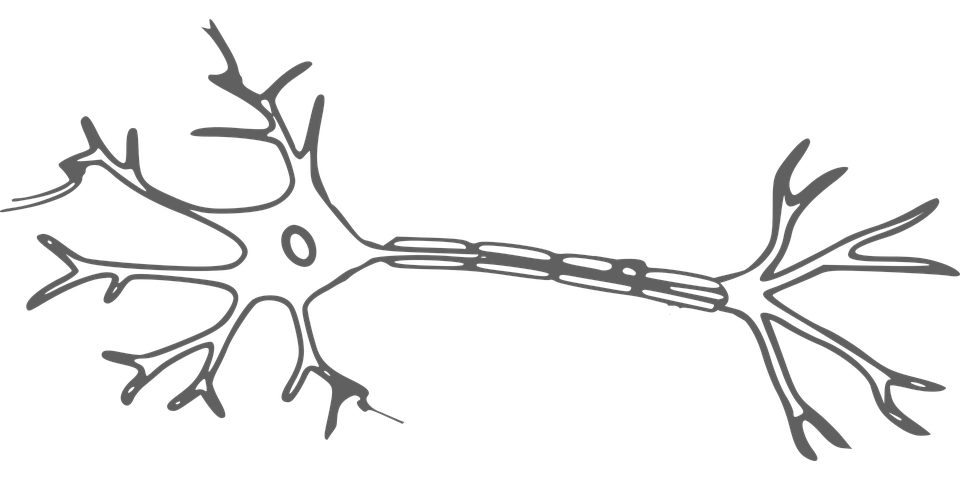
\includegraphics[width=0.8\linewidth]{figures/neuron}
    \caption{Parallelism between a real neuron and the artificial one used in \glspl{mlp}}
    \label{fig:back:neuron}
\end{figure}

Historically, this layer implemented a group of $m$ \emph{perceptrons}.
The perceptron~\cite{rosenblatt1958perceptron} is a biologically-inspired building block for artificial neural networks that has been developed mimicking the structure of biological neurons (see \ref{fig:back:neuron}).
As a neuron cell, it is composed by $n$ inputs $\x_i$ ($i=1 \dots n$), usually connected to the output of other neurons, and a single output $\mathbf{y}$ (axon).
Each input connection is associated with a weight $\w_i$ ($i=1 \dots n$) expressing how much of the signal coming through that connection is promoted or inhibited.
Weights in a perceptron are interpreted as the strength of the interconnection between neuron cells.
The neuron ``fires'' when the combination of their weighted inputs gets above a certain threshold;
this is modelled in the perceptron defining its output as the activation function $\a(\cdot)$ applied to the inner product between input and weights
%
\begin{equation}
    \y_j = \a \( \sum_{i=1}^n \w_i \x_i + b\) \,,
\end{equation}
%
where $\y_j$ is the output of a particular neuron and $b \in \R$ is an optional weight used as bias term.
% The weight vector $\w$ is tuned in the training phase in order to
A layer composed by $m$ perceptrons (and thus $m$ outputs $\y_j, j=1 \dots m$) sharing the same input $\x$ can be formalized with \ref{eq:back:fully-connected}, where the columns of $\W$ correspond to the weights of the $m$ perceptrons.
% Feed-forward artificial neural networks built stacking layers of perceptrons are called \glspl{mlp}.
In \glspl{mlp}, the outputs of a layer are densely connected to the input of each neuron comprising the next layer, hence the name ``fully-connected layer''.
The output of a \gls{mlp} with $L$ layers is defined as
%
\begin{equation}
    \y = \a \( \W_L \( \dots \a \( \W_2 \( \a \( \W_1 \x + \b_1 \) \) + \b_2 \) \) + \b_L \) \,,
\end{equation}
%
where $\(\W_i, \b_i \)$ are the parameters of the $i$-th fully-connected layer in the network.

\subsubsection{Convolutional Neural Networks}

\begin{figure}
    % TODO [FIG] example of crosscorr on image
    \centering
    \includegraphics[width=0.5\linewidth]{figures/cross-correlation2d}
    \caption{Example of cross-correlation between 2D signals}
    \label{fig:back:2d-cross-corr}
\end{figure}

A \gls{cnn} is a feed-forward artificial neural network composed by at least one \emph{convolutional} layer.
This kind of layer computes the cross-correlation between the input and a set of learnable filters.
Since there is a strong similarity between the convolution and the cross-correlation operations, this layer is often attributed with the adjective ``convolutional'' in the \gls{dl} literature;
thus we will adopt the same terminology throughout this thesis.

\paragraph{Cross-correlation}
The \emph{cross-correlation} (also called \emph{sliding inner product}) is typically used in signal processing to search for matches between two signals.
Intuitively, a small signal called \emph{filter} containing the prototype we want to match is slided on a bigger input signal, and for each position, the inner product between the intersection of the two signals measures the quality of the match.
We will provide the reader with the formulation of the two-dimensional version of the cross-correlation due to its massive adoption in image-related fields that are of interest for this work.

Given a two-dimensional input matrix $\x \in \R^{H \times W}$ and a two-dimensional filter $\w \in \R^{K_1 \times K_2}$, %with $K \ll \min(H,W)$,
the cross-correlation $\y \in \R^{H' \times W'}$ between $\x$ and $\w$ is given by
%
\begin{equation}\label{eq:back:cross-correlation}
    \y_{u,v} = \sum_{i=1}^{K_1} \sum_{j=1}^{K_2} \w_{i,j} \x_{i+u-1,j+v-1} \,,
\end{equation}
%
where $u = 1, \dots, H'$ and $v = 1, \dots W'$.
Intuitively, the filter $\w$ is superimposed on the input $\x$, and for each possible position $(u,v)$, the scalar product between the covered input and the filter is computed.
Depending on the presence of padding $P$ added to each side of the input and the stride $S$ of the filter application, the output dimensionality changes following the relations
\begin{equation} \label{eq:back:conv-size}
\begin{split}
    H' = \left \lfloor \frac{H + 2 \times P - K_1}{S} \right \rfloor + 1 \,,\quad
    W' &= \left \lfloor \frac{W + 2 \times P - K_2}{S} \right \rfloor + 1 \,.
\end{split}
\end{equation}
Inputs and outputs of convolutional layers are also called \emph{feature maps}, since high values in the two-dimensional map are usually interpreted as the presence of a feature a particular filter has learnt to identify.
A depiction of 2D cross-correlation is reported in~\ref{fig:back:2d-cross-corr}.

\begin{figure}
    \centering
    \includegraphics[width=\linewidth]{figures/convolution}
    \caption{Depiction of 2D cross-correlation on volumes implemented in convolutional layers}
    \label{fig:back:convolution}
\end{figure}

\paragraph{2D Cross-correlation on Volumes}
\ref{eq:back:cross-correlation} defines the cross-correlation operation for inputs and outputs having both a single feature map.
Images instead are represented as 3-D tensors having $C$ channels (e.g. $C=3$ for RGB data, $C=1$ for grayscale) and two spatial dimensions $H$ and $W$;
thus, the definition of the 2D cross-correlation is extended to 3D tensors letting the filters span the depth of the input tensor.
In such way, filters are still applied over the two spatial dimensions $H$ and $W$, but each output value depends on all the input feature maps in a particular spatial position.
Formally, given an input tensor $\x \in \R^{H \times W \times C}$ and a filter $\w \in \R^{K_1 \times K_2 \times C}$ the cross-correlation $\y \in \R^{H' \times W'}$ between $\x$ and $\w$ is defined as
%
\begin{equation}\label{eq:back:channel-cross-correlation}
    \y_{u,v} = \sum_{i=1}^{K_1} \sum_{j=1}^{K_2} \sum_{k=1}^C \w_{i,j,k} \x_{i+u-1,j+v-1,k} \,.
\end{equation}

A convolution layer is often composed by a bank of $K$ filters.
Each filter is applied to the input, obtaining $K$ output feature maps that are stacked along the depth dimension.
The obtained output is a new 3D tensor $\y \in \R^{H' \times W' \times K}$ that is commonly followed by an element-wise non-linear activation $\a(\cdot)$.
The entire process is depicted in \ref{fig:back:convolution}.

The main difference between fully-connected layers and convolutional layers is the way weights are utilized;
while fully-connected layers have a dedicated weight for each couple of input and output features, a convolutional layer shares the weights of its filters across the spatial dimensions, thus learning to detect translation-invariant features by design.

\paragraph{Pooling Layers}
Pooling layers are often used in \glspl{cnn} to reduce the amount of data to be processed in the next layers.
As the name suggests, this kind of layers pools data in groups and aggregates them using a non-parametric aggregation function, such as maximum or average.
The groups are defined as fixed-size windows that are slided along one or more dimensions of the data in the same way the cross-correlation operator is applied.
In the two-dimensional case, input and output sizes follow \ref{eq:back:conv-size}.
The application of convolutional layers having small strides usually produce redundant local information in their output.
Thus, a max-pooling layer is often used to reduce the resolution of intermediate feature maps.
% Instead, sum- and average-pooling are used to produce

\paragraph{Features hierarchy in \glspl{cnn}}
Convolutional layers are stacked to build deep \glspl{cnn}, that are the one of the core tools of Deep Learning for image perception and analysis~\cite{krizhevsky2012imagenet,sermanet2013overfeat,simonyan2014very,he2015delving,he2016deep,xie2017aggregated}.
Once trained, filters in a deep \gls{cnn} tend to organize in a hierarchy of detectors, where layers near the input detect the presence of simple features in the input data, while the following layers build up from them and detect more complex features.
A successful example of the representative power of \glspl{cnn} is object recognition.
% TODO [CITE] object hierarchical decomposition
The visual aspect of objects in images follow a hierarchical organization: an object can be decomposed in parts, parts in patches, patches in textures, textures in edges or blobs, and finally in pixels~\cite{}.
\begin{figure}
    % TODO [KEEP?] is feat hier figure valuable?
    \centering
    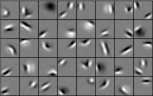
\includegraphics[height=2.9cm]{img/feat-hier-1.png}%
    \hfill%
    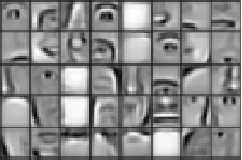
\includegraphics[height=2.9cm]{img/feat-hier-2.png}%
    \hfill%
    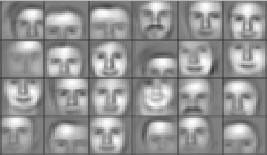
\includegraphics[height=2.9cm]{img/feat-hier-3.png}%
    \newline
    \caption{
    Visualization of the feature hierarchy learned by convolutional layers in a \gls{dl}-model trained on faces.
    Low-level features (edges and blobs, on the left) are detected and then combined to recognize parts (eyes, nose, mouth, in the middle) and finally faces (on the right).
    \figfrom{lee2011unsupervised}
    }
    \label{fig:back:filter-hier}
\end{figure}
\Glspl{cnn} trained to recognize objects, directly or indirectly, often organize their hierarchy of detectors following this kind of visual decomposition of objects (see \ref{fig:back:filter-hier}).


\subsection{Recurrent Neural Networks}
\label{subsec:back:rnn}

A \acrfull{rnn} is a stateful artificial neural network with feedback connections in which the output depends not only on the input, but also on the current state of the network~\cite{goodfellow2016deep,rumelhart1986learning}.
The state of the network acts as a memory which is updated at each input, allowing information to persist between inputs.
This architecture is naturally able to process sequences of inputs;
the elements of a sequence can be fed to the network one by one, updating the internal state of the network to compactly represent the sequence processed so far regardless of its length.
% This is achieved by adding a cycle in the computation graph --

\begin{figure}
    \centering
    \includegraphics[width=.9\linewidth]{figures/rnn}
    \caption{Basic architecture of a \acrlong{rnn} (left). On the right, its unrolled version for a sequence of length 5.}
    \label{fig:back:rnn}
\end{figure}

Given a sequence of inputs of length $T$ $\x_t \in \R^n, t = 1 \dots T$, and an initial state $\h_0 \in \R^m$, a \gls{rnn} can be described as a parametric function mapping the input and the state at a certain timestep to the next hidden state
%
\begin{equation}\label{eq:back:rnn}
    \h_t = f\(\x_t, \h_{t-1}; \W\) \,,
\end{equation}
%
where $f(\cdot)$ is the \emph{recurrent cell} of the \gls{rnn} parametrized by the weights $\W$, and $\h_t \in \R^m, t = 1 \dots T$ is the hidden state at timestep $t$, i.e.\ the state of the network after all inputs until $\x_t$ have been processed.
In its simplest form, the recurrent cell $f$ can be implemented using a fully-connected layer that operates
on the concatenation of the current state and input
%
\begin{equation}
    \h_t = \W [ \x_t | \h_{t-1} ] + \b \,,
\end{equation}
%
where $\W$ and $\b$ are the parameters of a fully-connected layer, and $[\cdot|\cdot]$ is the concatenation operation.
During learning, the \gls{rnn} is unrolled in time to the length of the input sequence to create an acyclic computation graph similar to \glspl{ffnn} (see \ref{fig:back:rnn}) on which standard training procedures can be applied (that will be discussed in \ref{subsec:back:optim}).
Depending on the task we want to model, we could be interested in the last hidden state $\h_T$ compactly represent the whole sequence, or we could use a combination of all hidden states $\h_i, i=1 \dots T$ to get access to the evolution of the information processed through time.

\paragraph{Bidirectional \glspl{rnn}}
In many tasks -- such as sequence classification and segmentation -- also the future context of the sequence is informative. However, \ref{eq:back:rnn} defines a \gls{rnn} encoding only past information, i.e.\   $\h_t$ depends only on information at time step $t' < t$.
To overcome this limitation, \emph{bidirectional} \glspl{rnn} have been proposed~\cite{schuster1997bidirectional}.
Bidirectional architectures adds a separate recurrent cell which process the sequence in reverse order (from future to past)
%
\begin{equation}
    \h'_t = f'\(\x_t, \h'_{t+1}; \W'\) \,,
\end{equation}
%
where $\h'_t$ encodes the "future" part of the sequence, i.e.\ depends on information at time step $t' > t$.
The concatenation of the internal states of both past-to-future and future-to-past \glspl{rnn} $[\h_t | \h'_t]$ is often used as the representation of the whole sequence.

\begin{figure}
    \centering
    \includegraphics[width=.9\linewidth]{figures/bidir-rnn}
    \caption{Unrolled version of a Bidirectional \gls{rnn} for a sequence of length 5}
    \label{fig:back:bidir-rnn}
\end{figure}

\subsubsection{Long Short-Term Memory}

\Gls{lstm}~\cite{hochreiter1997long} is a type of \gls{rnn} with a special formulation of the recurrent cell that has proved its effectiveness in several sequence-modeling tasks~\cite{graves2013speech,sutskever2014sequence,donahue2015long,vinyals2015show}.
This particular formulation is aimed at solving some major drawbacks of vanilla \glspl{rnn}, most importantly the inability to encode long-term dependencies in long sequences due to gradient instability problems, namely the problem of vanishing or exploding gradients ~\cite{pascanu2013difficulty}.
\Gls{lstm} cells are comprised by four learnable gating functions that better control the evolution of the internal state of the cell when dealing with long sequences, and mitigating problems occurring in vanilla RNNs, such as vanishing gradients~\cite{bayer2015learning}.

Let $\x_t \in \R^n$ an element of a sequence, and $\h_{t-1} \in \R^m$ the current hidden state.
The \emph{forget} gate $\f_t$ decides which information is to be discarded at the current step, and it is implemented as a fully-connected layer with $p$ output features and parameters $\w_f \in \R^{(n+m)\times p}, \b_f \in \R^p$ followed by a sigmoid activation
\begin{equation*}
    \f_t = \sigma\(\w_f [\h_{t-1} | \x_t] + \b_f\) \,.
\end{equation*}
The input gate $\i_t$ encodes the information that need to be inserted in the internal state of the cell $\c_t$, and it is implemented following the same rationale of the previous gate
\begin{equation*}
    \i_t = \sigma\(\w_i [\h_{t-1} | \x_t] + \b_i\) \,.
\end{equation*}
The update gate $\u_t$ modulates the amount of new input to be inserted in the internal state of the cell $\c_t$
\begin{equation*}
    \u_t = \tanh\(\w_u [\h_{t-1} | \x_t] + \b_u\) \,.
\end{equation*}
The new cell state $\c_t \in \R^p$ is computed as the sum of two terms;
the first one, given by the element-wise product ($*$) between the forget gate and the previous cell state, represents the part of the old state not to be forgotten;
the second one, computed as the element-wise product of the input and update gates, represent the modulated input to be kept in the new state;
\begin{equation*}
    \c_t = \f_t * \c_{t-1} + \i_t * \u_t \,.
\end{equation*}
The output gate $\o_t$ decides which information in the cell needs to be transferred to the final state $\h_t$
\begin{equation*}
    \o_t = \sigma\(\w_o [\h_{t-1} | \x_t] + \b_o\) \,,
\end{equation*}
and finally, the output state $\h_t$ is computed as
\begin{equation*}
    \h_t = \o_t * \tanh\(\c_t\) \,.
\end{equation*}
%
With an abuse of notation, the complete \gls{lstm} formulation can be compactly written as follows:

%\begin{align}\label{eq:back:lstm}
    % \begin{pmatrix} \i_t\\ \f_t \\ \o_t \\ \u_t \end{pmatrix}
%    \i_t &= \sigma\(\W_i [\h_{t-1} | \x_t] + \b_i\) \\
%    \f_t &= \sigma\(\W_f [\h_{t-1} | \x_t] + \b_f\) \\
%    \o_t &= \sigma\(\W_o [\h_{t-1} | \x_t] + \b_o\) \\
%    \u_t &= \tanh\(\W_u [\h_{t-1} | \x_t] + \b_u\) \\[2ex]
%    \c_t &= \f_t * \c_{t-1} + \i_t * \u_t \\
%    \h_t &= \o_t * \tanh\(\c_t\)
%\end{align}
\begin{align}\label{eq:back:lstm}
\begin{aligned}
    \begin{pmatrix} \i_t\\ \f_t \\ \o_t \\ \u_t \end{pmatrix} &=
    \begin{pmatrix} \sigma \\ \sigma \\ \sigma \\ \tanh \end{pmatrix}
    \( \W \begin{pmatrix} \x_t \\ \h_{t-1} \end{pmatrix} \) \\[2ex]
    \c_t &= \f_t * \c_{t-1} + \i_t * \u_t \\
    \h_t &= \o_t * \tanh\(\c_t\) \,,
\end{aligned}
\end{align}
%
where $\W \in \R^{(n+m) \times 4p}$ summarizes all the parameters of all the fully-connected layers forming the gates.
% TODO: [FIG] lstm?
A depiction of the \gls{lstm} cell is aslo available in \ref{fig:back:lstm}.

\begin{figure}
    \centering
    \includegraphics[width=\linewidth]{figures/lstm}
    \caption{Example of \gls{lstm} cell}
    \label{fig:back:lstm}
\end{figure}

\subsection{Loss Functions}
\label{subsec:back:loss}

Loss functions are a key component of \gls{ml} methods.
Its role is to quantitatively assign a value of goodness to a model in reference to the particular task we want to solve.

Given a training set $\X = \{\(\x_i, \y^\star_i\),\; i=1,\dots,N\}$ comprised by $N$ couples of inputs and desired outputs, the quality of a particular setting of parameters $\Theta$ is quantitatively defined by a \emph{loss function} $\L\(\X; \Theta\)$ that measures how much predictions and targets differ.
A loss function is usually defined as one of more terms summed together.
The main term $\L_d\(\X; \Theta\)$ is defined as the average of the individual loss values computed on each sample of the dataset $\L\(\y_i, \y^\star_i\)$ -- we denote it the \emph{data term}.
A secondary optional term $\L_r(\Theta)$ is often used to regularize the network and depends only on the model parameters $\Theta$ -- we indicate this as \emph{regularization term}.
Regularization consists of model constraints added to avoid other undesired properties during training such as \emph{overfitting} -- i.e. the tendency of a model to predict well known data while failing to make correct prediction for unseen data.
Regularization has gained importance in the \gls{dl} field due to the huge amount of parameters models are usually comprised of, thus increasing the risk of overfit on the train data.
The regularization term is usually multiplied by a hyperparameter $\alpha$ and then added to the loss function.
A general formulation of the loss function is
%
\begin{equation} \label{eq:back:loss}
\begin{aligned}
    \L\(\X; \Theta\) &= \overbrace{\L_d\(\X; \Theta\)}^{\textrm{data term}}&+\, \alpha &\overbrace{\L_r\(\Theta\)}^{\textrm{regularization term}}\\
                     &= \frac{1}{N} \sum_{i=1}^N \L\(\y_i, \y^\star_i\)&+\alpha & \,\quad \L_r\(\Theta\) \\
                     &= \frac{1}{N} \sum_{i=1}^N \L\(f\(\x_i; \Theta\), \y^\star_i\)&+\alpha & \,\quad\L_r\(\Theta\) \,.
\end{aligned}
\end{equation}
%
%where the optimal value of $\alpha depends on the absolute values of the loss terms and

In the next paragraphs, we will provide the reader with some of the most used formulations of $\L\(\y_i, \y^\star_i\)$ and $\L_r(\Theta)$ of interest for this work.

\paragraph{Mean Squared Error Loss}
When dealing with regression problems, we want our predictions to be close to the one or more real-valued targets.
For example, in an age estimation problem, we want our network to predict the exact age expressed as a real value, e.g. $46,5$.
The mean squared error between predictions $\z$ and targets $\z^\star$ is a commonly used loss function to measure the goodness of regressions
\begin{equation} \label{eq:back:mse}
    \L_\textrm{MSE}(\z, \z^\star) = \frac{1}{2} \( \z - \z^\star \)^2 \,.
\end{equation}
%
The scale factor $\frac{1}{2}$ is usually introduced to simplify the gradient computation when using this loss function (more details on this in \ref{subsec:back:optim}).

\paragraph{Cross-entropy Loss}
The cross-entropy loss is commonly used in \gls{ml} to measure the distance between two categorical distributions.
It is commonly adopted in single-label classification tasks, where a single label have to be assigned to a piece of data choosing from $N$ labels ($N \geq 2$).
Let $\z$ and $\z^\star$ the probability masses of two $N$-way categorical distributions, i.e. $\z_i, \z^\star_i \in [0,1],\; \sum_{i=1}^N \z_i = 1, \sum_{i=1}^N \z^\star_i = 1$;
the cross-entropy loss between the predicted distribution $\z$ and the target one $\z^\star$ is defined as
%
\begin{equation} \label{eq:back:cross-entropy}
    \L_\textrm{CE}(\z, \z^\star) = - \sum_{i=1}^N \z^\star_i \log \z_i \,.
\end{equation}
%
Classification models are often designed to output a $N$-dimensional vector $\z$ that is mapped to a categorical distribution via the \emph{softmax} function
%
\begin{equation} \label{eq:back:softmax}
    \textrm{softmax}(\z)_i = \frac{e^{\z_i}}{\sum_{j=1}^N e^{\z_j}} \,.
\end{equation}

\paragraph{$\mathbf{L_p}$ Weight Decay}
The most used regulatization terms in the \gls{dl} literature are the ones penalizing the parameters having large norm.
This is usually implemented defining the regularization term $\L_r\(\Theta\)$ added to the loss to be minimized as the $p$-norm of the parameters.
Practical definitions have been adopted for $p=2$ ($\mathbf{L_2}$ weight decay) and for $p=1$ ($\mathbf{L_1}$ weight decay).
The former produces a more uniform utilization of all the available parameters, penalizing under-utilized and over-utilized weights~\cite{ng2004feature}, and is defined as
%
\begin{equation} \label{eq:back:l2-weight-decay}
    \L_r\(\Theta\) = \frac{1}{2} ||\Theta||_2^2 = \frac{1}{2} \sum_i \theta_i^2 \,.
\end{equation}
%
The latter instead tends to produce a more sparse weight configuration, i.e. with many parameters having a null optimal value~\cite{ng2004feature}, and is defined as
%
\begin{equation} \label{eq:back:l1-weight-decay}
    \L_r\(\Theta\) = ||\Theta||_1 = \sum_i |\theta_i| \,.
\end{equation}

\subsection{Gradient-Based Optimization}
\label{subsec:back:optim}

As already stated, solutions of \ref{eq:back:optim} are the parameter configurations $\Theta$ that minimizes the loss function $\L$ defined over a given training set $\X$.
Unfortunately, in very rare cases closed-form solutions of \ref{eq:back:optim} are available for practical formulations of \gls{dl} models $f(\cdot)$ due to the non-linear non-convex nature of deep models.
In the past years, there was reluctance in the \gls{ml} field to work with non-convex models due to the lack of theoretical guarantees on their convergence.
Nevertheless, recent developments shown that non-convex model -- albeit having less guarantees -- have higher capacity and representational power and thus have a better overall performance~\cite{bengio2007scaling}.
The most common approach to find suboptimal (but valuable) solutions to \ref{eq:back:optim} is using iterative gradient-based optimization.

\paragraph{Gradient Descent}
In gradient-based optimization, given a training set $\X$ and a parameter configuration $\Theta$, we search for a new solution following the direction of the gradient of the loss function $\nabla\L\(\X, \Theta\)$ with respect to the parameters $\Theta$.
The direction given by $\nabla\L\(\X, \Theta\)$ is the one of maximum steepness of the loss surface in the parameter space, that is, the one that maximize the loss change locally.
A new parameter configuration $\Theta^\star$ is chosen \emph{descending} the loss surface along the direction of maximum steepness with a step size of $\lambda$, that is
%
\begin{equation} \label{eq:back:gradient-descent}
    \Theta^\star = \Theta - \lambda \nabla\L\(\X, \Theta\) \,.
\end{equation}
%
This update rule can be iterated until a (local or global) minimum of the loss function is reached.
This procedure is called \emph{gradient descent} optimization, and in the \gls{ml} field $\lambda$ is referred to as the \emph{learning rate}.
\begin{figure}
    \centering
    \includegraphics[width=\linewidth]{figures/gradient-descent}
    \caption{Example of gradient descent optimization on a loss surface $\L(\X)$ defined over a 2D parameter space $(\w_1, \w_2)$ with two different starting points}
    \label{fig:back:gradient-descent}
\end{figure}
A depiction of this algorithm for a 2D toy example is reported in \ref{fig:back:gradient-descent}.
Bigger learning rates correspond to bigger steps along the loss surface that usually improve the convergence rate and avoid local minima at the cost of a higher risk of oscillating around minimum points.
Small learning rates, instead, bring a lower convergence rate but are able to better exploit the local topology of the loss function, reaching a locally better solution.

\paragraph{Back-propagation}
As formalized in \ref{eq:back:deepnet}, \glspl{dnn} are comprised by many composition of non-linear functions $f_i$ each having its own set of parameters $\theta_i$.
Thus, to perform gradient descent on \gls{dl} models, we need to compute gradients $\nabla\L\(\X, \theta_i\)$ for each $\theta_i \in \Theta$.
This is efficiently done by \emph{back-propagation}~\cite{rumelhart1986learning,lecun1988theoretical}.

In back-propagation, we start computing the gradient of the loss function from the last layer (the one that produce the final predictions), and we propagate the error backwards to previous layers using the chain-rule for computing derivatives of compound functions.
For simplicity, we report the formulation of back-propagation for a \acrfull{ffnn}, but this mechanism is general and applies to all differentiable architectures.
Let $f(\x;\Theta)$ a \gls{ffnn} composed by $L$ layers with parameters $\Theta = \{\theta_1, \dots, \theta_L\}$ defined in \ref{eq:back:deepnet}, and let $\o_i$ the output of the $i$-th layer
\begin{equation}
\begin{split}
\o_0 &= \x \\
\o_i &= f_i \(\o_{i-1}; \theta_i \) \,.
\end{split}
\end{equation}
The gradient $\frac{\partial \L}{\partial \theta_i}$ of the loss function $\L$ with respect to $\theta_i$ can be decomposed using the chain-rule as
\begin{equation}
\begin{split}
    \frac{\partial \L}{\partial \theta_i} &= \frac{\partial \L}{\partial \o_i} \cdot \frac{\partial \o_i}{\partial \theta_i} \\
                                          &= \frac{\partial \L}{\partial \o_L} \cdot \frac{\partial \o_L}{\partial \o_{L-1}} \cdots  \frac{\partial \o_{i+1}}{\partial \o_i} \cdot \frac{\partial \o_i}{\partial \theta_i} \,,
\end{split}
\end{equation}
%
where the partial derivatives $\frac{\partial \o_{i+1}}{\partial \o_i}$ and $\frac{\partial \o_i}{\partial \theta_i}$ are well defined and depend on the implementation of the $i$-th layer $f_i$.
The formulations of the loss function $\L$ and intermediate layers $f_i$ are chosen to be differentiable to ensure that also the entire model -- being a composition of differentiable functions -- is in turn differentiable, and that back-propagation can be applied to efficiently compute gradients.


\paragraph{Stochastic Gradient Descent}
In our presentation of gradient-based optimization so far, the computation of the loss function $\L\(\X; \Theta\)$ and its gradient depend on the whole dataset $\X$.
This may be limiting for \gls{dl} applications where very large training sets are needed to train models, thus increasing the computational cost needed to compute the exact value of $\L\(\X; \Theta\)$.
To overcome this problem, \gls{sgd} and in particular mini-batch \gls{sgd}~\cite{rumelhart1986learning} have been proposed to compute an estimate the loss function and its gradients at a lower computational cost.

In mini-batch \gls{sgd}, we use a small random sample of the entire training set $ \tilde{\X} = \{ (\tilde{\x_i}, \tilde{\y_i}), i = 1 \dots B \} \subset \X$ (called \emph{batch} or \emph{mini-batch}) to compute an estimate of loss function
\begin{equation} \label{eq:back:minibatch-sgd}
\tilde{\L} \(\X; \Theta\) = \L (\tilde{\X}; \Theta) = \frac{1}{B} \sum_{i=1}^B \L(f(\tilde{\x_i}; \Theta), \tilde{\y_i}) \,,
\end{equation}
which in turn is used in back-propagation to estimate its gradient $\nabla \L(\tilde{\X}; \Theta)$ and perform the parameter update as specified in \ref{eq:back:gradient-descent}.
The size of the mini-batch size $B$ is a hyperparameter that controls the trade-off between the computational cost needed to compute the loss and the quality of the loss estimate.

\paragraph{\gls{sgd} with Momentum}
A successful proposal to improve the parameter update rule presented in \ref{eq:back:gradient-descent} is \gls{sgd} with \emph{momentum}~\cite{qian1999momentum}.
The key idea of momentum is to add to the current direction given by the loss gradient a fraction of the direction computed in the previous iteration, such that the direction we are following to descend the loss surface gains inertia and smooths out eventual oscillations given by very steep loss manifolds.
Given $\m^{(k-1)}$ the direction of the previous iteration, we define the new direction to follow $\m^{(k)}$ as
\begin{equation} \label{eq:back:momentum}
\begin{aligned}
    \m^{(0)} &= 0 \\
    \m^{(k)} &= \gamma \m^{(k-1)} + \nabla\L\(\X; \Theta^{(k)}\) \\
    \Theta^{(k+1)} &= \Theta^{(k)} - \lambda \m^{(k)} \,,
\end{aligned}
\end{equation}
%
where $\gamma \in (0,1)$ is the momentum of the previous direction.
Commonly used values for $\gamma$ are around $0.9$.
A good analogy to comprehend the rationale behind momentum is a ball pushed down a hill:
the higher the momentum $\gamma$, the more inertia the ball has, and the less it is influenced by steepness variations during the descent.
This modified update rule tends to discard the oscillating directions of the gradient while strengthening the stable directions over iterations;
this brings a reduction of oscillations while descending the loss manifold and thus a faster convergence.

\paragraph{Adam}
Another widely used parameter update rule in the \gls{dl} literature is \gls{adam}~\cite{kingma2014adam}.
Similar to other proposed update rules (such as Adagrad~\cite{duchi2011adaptive} or Adadelta~\cite{zeiler2012adadelta}), this method computes an adaptive learning rate for each parameter to be optimized based on the second moment of the gradients $\v$ (i.e. squared gradients), but in addition, it also estimates the first moment $\m$ (the mean of the gradient itself) as in \gls{sgd} with momentum
%
\begin{equation} \label{eq:back:adam-moments}
\begin{aligned}
    \m^{(k)} &= \beta_1  \m^{(k-1)} + \(1 - \beta_1 \)  \nabla\L\(\X; \Theta^{(k)}\) \\
    \v^{(k)} &= \beta_2  \v^{(k-1)} + \(1 - \beta_2 \)  \nabla\L\(\X; \Theta^{(k)}\)^2 \,.
\end{aligned}
\end{equation}
%
The hyperparameters $\beta_1$ and $\beta_2$ are respectively controlling the aggressiveness of the exponential average of the two moments $m^{(k)}$ and $v^{(k)}$.
Since the initial values of the moments are initialized to zero, the authors propose to use the bias-corrected version of the moments, that is
%
\begin{equation} \label{eq:back:adam-moments-bias}
\begin{aligned}
    \hat{\m}^{(k)} &= \frac{\m^{(k)}}{1 - \beta_1^k} \\
    \hat{\v}^{(k)} &= \frac{\v^{(k)}}{1 - \beta_2^k} \,.
\end{aligned}
\end{equation}
%
Finally, moments estimates are used to formulate the \gls{adam} update rule
%
\begin{equation} \label{eq:back:adam}
\theta^{(k+1)}_i &= \theta^{(k)}_i - \frac{\lambda}{\sqrt{\hat{\v}^{(k)}_i} + \epsilon} \m^{(k)}_i \qquad \forall \theta_i \in \Theta \,,
\end{equation}
%
where $\m^{(k)}_i$ and $\hat{\v}^{(k)}_i$ are the first and second moments estimates of the gradients corresponding to parameter $\theta_i$, and $\epsilon$ is a small values to prevent division by zero.
Commonly used values for hyperparameters are $\beta_1 = 0.9$, $\beta_2 = 0.999$, and $\epsilon = 10^{-8}$, as suggested by the authors.


% TODO move dropout?
\paragraph{Dropout}
Regularization is not limited to regularization loss terms only.
\emph{Dropout}~\cite{hinton2012improving} is a common regularization technique for \glspl{dnn} which consists in deactivatating (drop) some neurons of an internal layer (by setting their activations to zero) during the training phase and thus enabling the back-propagation of the error only in the survived neurons.
The choice of the neurons to deactivate is random: each neuron on which dropout is applied has a given probability $p$ to survive.
The employment of this technique usually increases the number of training iterations needed to a model to converge, because only the subset of weights of the survived neuron are updated in an optimization step.
However, training a random subset of neurons at each iteration reduces the co-adaptation of neurons, which tend to learn a more diversified and independent configurations of weights.
This results in a increased ability of bigger models to exploit their capacity and limit overfit.
At test time, all neurons are used, virtually exploiting and combining the predictions of many independently trained models.
The activations of the layers trained with dropout are scaled by $p$ to approximate the combined prediction produced by the virtual ensemble of sub-networks.


\section{Image Classification}
\label{sec:back:image-classification}

% TODO intro to img classification, examples and applications
% Examples (simple classif., sentiment analysis, etc.)
% Classifying images is super cool bla bla
In this section, we formally define the problem of image classification, and we analyze and review recent solutions based on \acrlong{dl} -- in particular Deep \acrlongpl{cnn} -- proposed in the literature.

% TODO sentence dropped here at random
In the case of image classification, the data on which classifiers must rely on is raw pixel data, usually organized in a tensor with shape $(H, W, C)$, respectively representing the height, the width, and the number of channels of the image.

Many real-world problems in image understanding, such as object and face recognition, anomaly detection, and ..., can be formalized as classification problems.
For this reason, classification methods for images have received an increasing attention in the last decade.

\subsection{Problem Setting}
\label{subsec:back:classification}
Image classification consists of assigning one or more labels to an image $\x$ choosing from a finite set of $L$ labels.
We refer to \emph{single-label} $L$-way classification if only one label has to be picked among the $L$ available, referring to the special case in which $L=2$ as \emph{binary} classification.
If multiple labels can be assigned to a piece of data, we talk about \emph{multi-label} classification.
A multi-label $L$-way classification problem is often decomposed in $L$ independent binary classification sub-problems, each of them focusing on predicting the presence or the absence of one of the available $L$ labels.

Let $I$ the image space;
given an image to be classified $\x \in I$, a single-label $L$-way classifier is a function $f$ mapping $\x$ into the label space.
% Solving a classification problem reduces to find a suitable classifier $f$ that agrees with observed data labels.
The commonly used form of classification is \emph{probabilistic}, in the sense that soft assignments to the available labels are considered instead of hard ones.
In this case, an image $\x$ is mapped into its posterior probability $p_i = p(\y = i | \x)$ of belonging to category $i$, for each category $i \in \{1, \dots, L\}$.
Thus, the classifier is a function $f: I \to \p$ which maps an image to the parameters $\p = (p_1, \ldots, p_L), \sum_{i=1}^L p_i = 1$ of a categorical distribution defined over the label space.
Soft assignments present a broad range of advantages with respect to hard assignments, the most important one being differentiability, which enables and facilitates gradient-based learning of models for $f$.

% TODO expand image classification problem setting?

\subsection{Evaluation}
\label{subsec:back:classif-eval}

In this section, we will report the most commonly used evaluation metrics to measure the quality of classification models.
Assume $\Y = (y_1, \ldots, y_n)$ is a set of predictions and $\tilde{\Y} = (\tilde{y}_1, \ldots, \tilde{y}_n)$ the set of the ground-truth labels for a single-label $L$-way classification problem, with $y_i, \tilde{y}_i \in \{1, \ldots, L\}$. % for $i \in \{1, \ldots, N\}$.

\paragraph{Confusion Matrix}
One of the fundamental tools for evaluating a set of label assignments is the \emph{confusion matrix} $C = \{c_{ij}\}$, which compactly reports the co-occurence of predicted and ground-truth labels.
The element $c_{ij}$ of the matrix indicates the number of times the model predicted the class $i$ for a sample belonging to class $j$.
We report in \ref{tab:back:confusion} the confusion matrix for the binary case ($L=2$) together with the terminology used to refer to particular values in the matrix.
For the binary case, many useful metrics can be computed from the confusion matrix, and we will introduce some of them in the next paragraphs.
Notice that the same metrics can be applied to cases with $L > 2$ by reformulating them as $L$ binary problems, where one class is the positive class, and the other $(L-1)$ are condensed in the negative class;
metrics can be computed considering each class as the positive one and then aggregated to obtain a global metric for the classification.

\begin{table}
\newcolumntype{M}[1]{>{\centering\arraybackslash}m{#1}}
\renewcommand{\arraystretch}{1.5}

\begin{tabularx}{\linewidth}{cr|M{1.3cm}|M{1.3cm}|>{\hskip 2cm}r@{\hskip 3pt}X}
\multicolumn{4}{c}{}                                                                                                                                      & $\mathrm{TP}=$ & True Positives, i.e. correct hits           \\
\multicolumn{2}{c}{}                                                  & \multicolumn{2}{c}{\bfseries Actual class}                                        & $\mathrm{TN}=$ & True Negatives, i.e. correct rejections     \\
\multicolumn{2}{c}{}                                                  & \multicolumn{1}{c}{\itshape \small Positive} & \multicolumn{1}{c}{\itshape \small Negative} & $\mathrm{FP}=$ & False Positives, i.e. false alarms          \\ \cline{3-4}
\parbox[t]{2mm}{\multirow{2}{*}{\rotatebox[origin=c]{90}{\bfseries Predicted}}} & {\itshape \small Positive} & $\mathrm{TP}$ & $\mathrm{FP}$                   & $\mathrm{FN}=$ & False Negatives, i.e. misses                \\ \cline{3-4}
                                                                      & {\itshape \small Negative}           & $\mathrm{FN}$ & $\mathrm{TN}$                   &  $\mathrm{P}=$ & $\mathrm{TP}+\mathrm{FN}=$ Positive samples \\ \cline{3-4}
\multicolumn{4}{c}{}                                                                                                                                      &  $\mathrm{N}=$ & $\mathrm{TN}+\mathrm{FP}=$ Negative samples \\
\end{tabularx}

\caption{Confusion matrix for a binary classification problem and the related terminology}
\label{tab:back:confusion}
\end{table}

% Accuracy
\paragraph{Accuracy} The accuracy of a classification is defined for the binary case as
\begin{equation} \label{eq:back:accuracy-binary}
    \mathrm{Acc.} = \frac{\mathrm{TP} + \mathrm{TN}}{\mathrm{P} + \mathrm{N}} = \frac{\mathrm{TP} + \mathrm{TN}}{\mathrm{TP} + \mathrm{FN} + \mathrm{TN} + \mathrm{FP}} \,,
\end{equation}
that is the fraction of correctly classified samples.
For the general case with more than two classes, the accuracy is given by the sum of the elements on the diagonal of the confusion matrix -- which contains the counts for correct predictions -- and the total number of classified samples
\begin{equation} \label{eq:back:accuracy}
    \mathrm{Acc.} = \frac{\sum_{i=1}^L c_{ii}}{|Y|} \,.
\end{equation}

% Top-K Accuracy
\paragraph{Top-$K$ Accuracy}
A common variant of the accuracy often used for probabilistic classifiers when many classes are considered, is the \emph{Top-$K$ Accuracy}.
Given the $L$ probabilities (or scores) assigned to a sample by a probabilistic classifier, we consider the prediction correct if the ground-truth class appears in the first $K$ highest scored classes.
The metric then is computed as the fraction of correct predictions.

The accuracy metric is a very simple and intuitive metric for evaluating classifiers, but it may be misleading when employed on unbalanced test sets.
Consider for example a binary classification example with 95 positive and 5 negative samples;
A classifier always predicting the positive class (a trivial acceptor) achieves an accuracy of $.95$ while behaving very poorly on negative classes.
In this scenarios, other ratios derived from the classification matrix are used to better characterize the performances of a classifier.

% TPR TNR
\paragraph{\acrshort{tpr} and \acrshort{tnr}}
The \emph{\gls{tpr}} is the ratio between correctly predicted positive samples and the number of actual positive samples
\begin{equation} \label{eq:back:tpr}
    \mathrm{TPR} = \frac{\mathrm{TP}}{\mathrm{P}} = \frac{\mathrm{TP}}{\mathrm{TP} + \mathrm{FN}} \,.
\end{equation}
It is also known as \emph{Recall} of the positive class, as it indicates the fraction of positive samples correctly accepted as positive.
Similarly, the \gls{tnr} represent the same concept applied to the negative class, and it is defined as
\begin{equation} \label{eq:back:tnr}
    \mathrm{TNR} = \frac{\mathrm{TN}}{\mathrm{N}} = \frac{\mathrm{TN}}{\mathrm{TN} + \mathrm{FP}} \,.
\end{equation}

% FNR FPR
\paragraph{\acrshort{fnr} and \acrshort{fpr}}
While \gls{tpr} and \gls{tnr} measure how well a classifier perform on both classes, the \gls{fnr} and \gls{fpr} are complementary measures that indicate instead the faction of classification errors.
Specifically, the \gls{fnr} is defined as the fraction of positive examples wrongly classified as negatives, and it is complementary to the \gls{tpr}
\begin{equation} \label{eq:back:fnr}
    \mathrm{FNR} = \frac{\mathrm{FN}}{\mathrm{P}} = \frac{\mathrm{FN}}{\mathrm{TP} + \mathrm{FN}} = 1 - \mathrm{TPR}\,.
\end{equation}
Similarly, the \gls{fpr} measures the fraction of errors on the negative class
\begin{equation} \label{eq:back:fpr}
    \mathrm{FPR} = \frac{\mathrm{FP}}{\mathrm{N}} = \frac{\mathrm{FP}}{\mathrm{TN} + \mathrm{FP}} = 1 - \mathrm{TNR}\,.
\end{equation}

\paragraph{\acrshort{roc} and \acrshort{auc}}
Probabilistic classifiers produce soft assignments of each sample to the available classes in the form of scores or confidences from which the final hard classification is obtained.
A common way to do so is to use an acceptance threshold, and depending on the choice of the threshold, the performance of the classifier may vary substantially.
A useful tool to evaluate the performance of the classifier in relation to the threshold is the \gls{roc} plot~\cite{fawcett2006introduction}.
Each point on a \gls{roc} plot represents the performance of the classifier for a given threshold $T$, and has as coordinates the \gls{fpr}$(T)$ (on the x-axis) and the \gls{tpr}$(T)$ (on y-axis) obtained by using $T$.
An optimal classifier lies on the top-left point $(0,1)$, while a random-chance classifier lies on the $TPR = FPR$ line.
A \gls{roc} curve for a given classifier is comprised by all the points obtained by varying the threshold.
The curve starts from $(0,0)$ -- that correspond to having the most stringent threshold, thus a trivial rejector classifier -- and ends in $(1,1)$ -- corresponding to the most permissive threshold that results in a trivial acceptor.
\Gls{roc} curves enables a visual comparison of classifiers, since curves lying closer to the optimal $(0,1)$ point are considered better classifiers independently from the particular threshold chosen.
To quantitatively compare classifiers on the \gls{roc} plane, the \gls{auc} is often computed as a unique threshold-independent metric;
the higher the \gls{roc} curve, the closer the \gls{auc} is to $1$ (see \ref{fig:back:roc}).

\begin{figure}
    \centering
    \includegraphics[width=\linewidth]{figures/roc-example}
    \caption{Example of \acrfull{roc} curves for two binary classifiers, and the relation between their corresponding \acrfullpl{auc}. }
    \label{fig:back:roc}
\end{figure}

\paragraph{\acrshort{eer} Accuracy}
Another useful threshold-independent metric which is commonly used to compare classifiers is the \gls{eer} accuracy.
This is the accuracy obtained by choosing the threshold yielding an equal error rate on both positive and negative classes, i.e.
\begin{equation} \label{eq:back:eer-accuracy}
    \mathrm{EER\ Acc.} = \mathrm{Acc}(T) \quad | \quad \mathrm{FPR}(T) = \mathrm{FNR}(T) \,,
\end{equation}
where $\mathrm{Acc}(T)$, $\mathrm{FPR}(T)$, and $\mathrm{FNR}(T)$ indicates respectively the accuracy, the \gls{fpr}, and the \gls{fnr} obtained using $T$ as threshold.
On the \gls{roc} plot, this threshold setting corresponds to the point where the classifier curve intersect the second diagonal of the unit square, i.e. the $\mathrm{TPR} = 1 - \mathrm{FPR}$ line, which is equivalent to $\mathrm{FPR} = \mathrm{FNR}$ by substituting \ref{eq:back:fnr} in \ref{eq:back:eer-accuracy}.

\subsection{Relevant works}
\label{subsec:back:classif-relwork}

\paragraph{Before \acrlong{dl}}
% TODO divide f in features and classifier, manually (?)
Traditional approaches to image classification required to manually design the classifier $f(\cdot)$.
% ESWA: The traditional approaches to the classification problem use ad-hoc functions to extract from an image specific features that are considered to be indicative of certain objects.
In particular, hand-crafted features detectors and descriptors -- such as SIFT~\cite{lowe2004distinctive}, SURF~\cite{bay2006surf}, ORB~\cite{rublee2011orb}, MSER~\cite{matas2004robust}, KAZE~\cite{alcantarilla2012kaze} to cite some -- were employed to extract information from the image considered indicative for the presence of certain objects.
For example, the presence of features like hard corners and straight edges might indicate man-made objects in the image~\cite{piccinini2012real}.
Shallow classifiers based on \gls{ml} methods -- such as logistic regressors~\cite{mensink2012metric} or \glspl{svm}~\cite{arandjelovic2012three} -- then relied on these extracted features and their aggregation (VLAD~\cite{jegou2010aggregating}, Fisher Vectors~\cite{perronnin2010improving}) to determine which label to be assigned to the image.

% ESWA: it is hard to think of general, robust, reliable features, which map to specific object types; - it is a huge task to find the right combination; - of features for every type of object to classify; - it is difficult to design functions that are robust to translations, rotations and scaling of objects in the image
% ESWA: All these problems make developing high accuracy object detectors and classifiers for a broad range of objects very hard.
However, manually engineered solutions are feasible for very specific problems -- such as image stitching~\cite{brown2007automatic} and 3d reconstruction~\cite{schonberger2016structure} -- where the conditions are well known and modelled.
In general, thinking of features that are invariant to transformations, reliable for many types of objects, and robust to noise and other exogenous factors is often very difficult and time-consuming.
% ESWA: it is often very complex to develop robust and reliable feature detectors and descriptors by hand.
% TODO better definition of VSA
As an example, consider the problem of visual sentiment analysis (further discussed in \ref{ch:cross-learning}), which, in a nutshell, consists in detecting the emotions conveyed by images.
Manually defining a good set of features to extract from images to solve this task is a cumbersome process and usually leads to suboptimal solutions.

\paragraph{ImageNet Challenge and the Deep Learning era}

\begin{table}
    \begin{tabularx}{\linewidth}{p{4.5cm}X>{\centering}c}
        \toprule
        \textbf{Team} & \textbf{Image Features} & \textbf{Error} \\
        \midrule
        \emph{LEAR}~\citep{mensink2012metric} \newline {\footnotesize LEAR INRIA Grenoble} \newline {\footnotesize TVPA Xerox Research Centre Europe} & PCA-reduced FV + dense SIFT & 34.5 \\ % -
        \midrule
        \emph{UvA}~\citep{sanchez2011high} % ,scheirer2012multi}
        \newline {\footnotesize University of Amsterdam} & Compressed FV + SIFT & 29.6 \\ % -
        \midrule
        \emph{XRCE}~\citep{akata2014good} \newline {\footnotesize Xerox Research Centre Europe} \newline {\footnotesize LEAR INRIA} & FV / BOV + multi-scale dense SIFT  & 27.1 \\ % -
        \midrule
        \emph{VGG}~\citep{arandjelovic2012three,sanchez2012modeling} \newline {\footnotesize University of Oxford} & SVM on FV + dense rootSIFT + Color statistics & 27.0 \\ % 50.0
        \midrule
        \emph{ISI}~\citep{harada2012graphical} \newline {\footnotesize University of Tokyo, JST PRESTO} & Gaphical Gaussian Vectors + dense SIFT & 26.2 \\% 53.6
        \midrule
        \emph{SuperVision}~\citep{krizhevsky2012imagenet} \newline {\footnotesize University of Toronto} & Trained features (AlexNet \gls{cnn}) & \textbf{16.4} \\ % 34.2
        \bottomrule
    \end{tabularx}
    \caption{ILSVRC12 leaderboard reporting the accuracy (as top-5 error percentage) on the image classification task obtained by the participating teams. Results taken from~\cite{russakovsky2015imagenet}}
    \label{tab:ilsvrc12-results}
\end{table}

% ESWA: The Deep Learning approach, on the other hand, exploits a large number of ground-truth labeled data to discover which features and combinations of features are most discriminative for each class of objects to be recognized, and builds a combined feature extraction and classification model.
On the other hand, \acrlong{dl} approaches rely on large amount of labeled data to automatically discover which features and combination of them are important for the task.
The main advantage of this kind of approach is its general applicability even to large-scale scenarios where thousands of different classes of images have to be recognized.
Recent results in the \gls{ilsvrc} are a striking evidence of the success of \gls{dl} methods in image classification.
\gls{ilsvrc} is an annual challenge in which competitors are asked to recognize generic objects in images and classify them accordingly choosing from a vast label space (in the order of 1,000 labels).
Before \gls{dl} methods were applied in this competition, leading solutions were based on combinations and aggregation of hand-made local features~\cite{harada2012graphical,akata2014good,sanchez2011high,mensink2012metric}.
Interestingly, in the edition of the challenge occurred in 2012, a \gls{dl} method based on \acrlongpl{cnn}~\cite{krizhevsky2012imagenet} outperformed non-\gls{dl} solutions by a large margin ($16.4 \%$ top-5 error vs $26.2 \%$ of the second place, see \ref{tab:ilsvrc12-results}), marking the beginning of the \gls{dl}-era in the computer vision field.
Since then, we experienced an exponential growth of interest by research communities in \gls{dl} technologies.
While the theories and concepts behind \gls{dl} approaches -- such as artificial neural networks and \acrlong{ml} -- were already studied and formalized in the past~\cite{rosenblatt1958perceptron,rumelhart1985learning,lecun1989backpropagation,widrow199030}, in the last years, the combination of different factors has allowed \acrlong{dl} to flourish.
Most importantly, huge amounts of data -- collected and labeled exploiting Web technologies and crowd-sourcing -- provided the supervision needed by very deep models having millions of parameters to properly train, and modern hardware and accelerators -- such as \glspl{gpu} -- provided the computing power needed to speed up training and evaluation procedures.

%ILSVRC winners (Hybrid, VGG, Inception, Residual, ResNeXT, SENets?)
\paragraph{AlexNet}
% Krizhevsky et al., 2012
We start our review of relevant work in image classification right from the method that won the \gls{ilsvrc}'12 challenge, that is the \gls{dcnn} proposed by~\citet{krizhevsky2012imagenet}, also knwon as \emph{AlexNet}.
Inspired by previous work on handwritten digits recognition~\cite{lecun1989backpropagation}, the AlexNet model is composed by a deep convolutional neural network that maps directly RGB data to labels without relying on explicit feature engineering.
It is comprised by 5 convolutional layers with \gls{relu} activation, the first three of them interleaved with overlapping max-pooling operations to reduce the resolution of intermediate feature maps.
This first part of the network is responsible to learn and extract good features, and it is followed by a classification sub-network consisted of three fully-connected layers with a final softmax transformation that maps the outputs to probabilities in the label space.
The whole network -- both the feature extractor and the classifier -- has roughly 60 million parameters and 650,000 neurons, and it is trained end-to-end;
it took initially two weeks on two GPUs to the authors to train the model with the 1.2 million images provided by the \gls{ilsvrc}'12 train set.
More details about the architecture are reported in \ref{fig:back:alexnet}.
Another key ingredient of the success of this architecture is the application of \emph{dropout}~\cite{hinton2012improving} to fully-connected layers, which permitted to the authors to drastically reduce overfitting.
AlexNet won the \gls{ilsvrc}'12 competition with roughly a 10\% gap in error from the second place competitor.
This amazing results provided a springboard for the research community for a new way to to do image classification and more in general to learn high-quality features for images.
In the following years, many other researchers developed \glspl{cnn} for image classification or similar vision tasks, reaching always smaller error rates on important challenges such \gls{ilsvrc}.

\begin{figure}
    \centering
    % TODO alexnet figure
    \includegraphics[width=\linewidth]{figures/alexnet}
    \caption{Architecture of the AlexNet \gls{cnn}.}
    \label{fig:back:alexnet}
\end{figure}

\paragraph{ZFNet} Despite \glspl{cnn} being remarkably good in solving vision task,
trained feature detectors in deep models tend to be difficult comprehend and explain.
%it is common to treat them as black boxes without having a clear understanding of its internals.
To alleviate this problem, \citet{zeiler2014visualizing} proposed a visualization technique based on deconvolutions to shed light on the representations learned by intermediate convolutional layers.
\ref{fig:back:filter-visualization} shows an example of the proposed approach applied on a trained model.
The usage of these visualizations lead the authors to debug the AlexNet architecture and to propose a new one, informally called \emph{ZFNet} in the research community, which incorporates some modifications, namely the reduction of the size and stride of the filters of the first layer, that enables the model to learn a more balanced set of feature extractors.
This improved architectures won the \gls{ilsvrc}'13 classification task with a $11.7 \%$ top-5 error.

\begin{figure}
    \centering
    % TODO add deconvolution figure from zeiler2014visualizing, big figure or fig 6?
    \includegraphics[width=\linewidth]{img/filter-visualization}
    \caption{Visualization of the top 9 most activated neurons in ....}
    \label{fig:back:filter-visualization}
\end{figure}

\paragraph{OverFeat} \citet{sermanet2013overfeat} proposed \emph{OverFeat}, a modification of the AlexNet architecture optimized also for object localization and detection in images, where the model is asked to predict also the bounding boxes of the object of interest.
The authors proposed two different architectures: a \emph{fast} model having the same architecture of AlexNet with different parameters, i.e. a smaller stride in the first convolutional layers and non-overlapping max-pool operations, and a \emph{accurate} model counting an additional convolution layer, a higher number of output features and smaller strides.

\paragraph{VGG Net} % Simonyan & Zisserman, 2014
\citet{simonyan2014very} of the \gls{vgg} of Oxford University studied the effects of the depth of convolutional networks for large-scale image classification.
Employing small 3$\times$3 kernels for convolutions allowed them to stack more layers while keeping roughly the same amount of parameters.
They proposed deeper architectures comprised by up to 19 learnable layers and demonstrated that the increased depth of \glspl{cnn} is beneficial for the classification accuracy.
Their best-performing network composed by 19 layers achieved the second place in the \gls{ilsvrc}'14 classification task with $7.3 \%$ a top-5 error.
In this work, we will refer to the best-performing architectures, namely the 16-layer and 19-layer ones, respectively as \gls{vgg}-16 and \gls{vgg}-19.

% Girshick et al., 2014
\paragraph{Inception}
While increasing the depth of networks continued to increase the performance, the major drawbacks of deeper models were the larger model size -- that makes the network more prone to overfitting -- and an increased computational budget.
\citet{szegedy2015going} proposed to improve the efficiency of the network employing a novel architectural block called \emph{Inception module}.
To better utilize the capacity of the model, this module extracts multiple-scale features by applying different-sized convolutions ``in parallel'' to the input feature maps and concatenating them.
Moreover, 1x1 convolutions and max-pooling operations are used as a way to reduce -- both in terms of number of feature maps and spatial resolution -- the inputs of costly operations, such as the bigger 5x5 convolutions.
The usage of this module permitted to increase both the width and the depth of networks without adding a substantial computational overhead.
The first network architecture leveraging Inception modules proposed by the authors, called GoogLeNet, is composed by 19 learnable layers, but it has 12 times fewer parameters with respect to AlexNet while being significantly more accurate, as demonstrated by its first place in the \gls{ilsvrc}'14 classification leaderboard.

% TODO add BatchNorm paper? together with DropOut \cite{ioffe2015batch}

\paragraph{Residual Networks}

Despite having more capacity, deeper models are more prone to optimization problems.
Due to the inability to fully exploit the parameters of additional layers, the possibility to arbitrarily increase the capacity of the model to solve more complex problems is often limited, and after a certain number of layers the performance of the model start decreasing instead of remaining constant.
\citet{he2016deep} strongly alleviated this problem by introducing \emph{residual learning} of deep models.
Instead of modelling directly the mapping $g$ between input $\x$ and output $\y = g(\x, \w)$ performed by a layer, the authors proposed to model and learn the residual mapping between input and output, i.e. $\y = \x + g(\x, \w)$.
In this settings, it is easier for a layer to model the identity transformation simply pushing its weights $\w$ toward zero.
Thus, additional layers may not introduce unstable transformations that limit the exploitation of the capacity of the network.
Residual learning can be easily implemented in \gls{dcnn} by adding skip-connections in its computational graph;
this kind of architectures are called \glspl{resnet}.
The authors proposed multiple \glspl{resnet} with an increasing number of layers.
Due to its increased depth, the number of filters of convolution layers can be reduced, requiring a low computational budget.
\gls{resnet}-152 -- their best-performing 152-layer model -- won the \gls{ilsvrc}'15 classification task with a top-5 error of $3.57 \%$, while having a computation cost of roughly 11 billion FLOPs (still lower than the 19 billion FLOPs of \gls{vgg}-19).
On smaller datasets, such as CIFAR-10 and CIFAR-100, the authors experimented with up to 1,000-layers networks when overfitting occurred.
The extended generalization power of deeper representations lead this architectures to win in a number of challenging vision competitions, such as the \gls{ilsvrc} 2015 classification, detection and localization tasks, and the \acrshort{coco} 2015 detection and segmentation tasks.

\paragraph{Beyond \glspl{resnet}}
Residual learning and \glspl{resnet} represent the last significant breakthrough in \gls{dnn} and feature learning.
In the last years, many smaller improvements have been made by developing new ideas based on the ones already reviewed.
\citet{huang2017densely} presented DenseNets, an evolution of \glspl{resnet} where skip-connections are used to connect every layer to every succeeding layer inside a block in a dense manner.
In~\cite{szegedy2017inception}, the authors revisited the Inception module adding residual connections, and proposed the Inception-ResNet architecture.
Similarly, \citet{xie2017aggregated} improved the residual blocks of \glspl{ResNet} by splitting convolutional layers into smaller convolutions applied in parallel, in a similar way the Inception module did;
the obtained architecture, dubbed ResNeXt, reduces the computational load while keeping the same representative power.

At the time of writing, one of the most recent work improving \glspl{dcnn} for image classification and recognition is \glspl{senet}~\cite{hu2017squeeze}.
A new architectural block -- called Squeeze-and-Excitation (SE) block -- has been proposed to better model the inter-dependencies between features map in convolutional layers.
In a nutshell, a SE block is designed as a gating function that weights and recalibrates each input feature map;
a \emph{squeeze} operation aggregates feature maps in the spatial dimensions, and the following \emph{excitation} operation relies on this information to produce the weights for recalibration via a per-channel sigmoid function;
feature maps are then multiplied by this set of weights to obtain the recalibrated output.
With a minimal additional computation cost, this block can be applied to convolutions or set of convolutions in \glspl{cnn} to improve their generalization power.
A small ensemble of SENet-154 -- a modified version of a ResNeXt-152 network~\cite{xie2017aggregated} equipped with SE blocks -- won the first place in the \gls{ilsvrc}'17 classification challenge with a top-5 error of $2.25 \%$.

% ESWA :
% A Deep Learning approach particularly effective for vision tasks exploits Convolutional Neural Networks (CNN) (Krizhevsky et al., 2012; Simonyan & Zisserman, 2014; Girshick et al., 2014).
% A CNN is composed of a possibly large number of hidden layers, each of which performs mathematical computations on the input provided by the previous layer and produces an output that is given in input to the following layer.
% A CNN differs from classical neural networks for the presence of convolutional layers, which can better model and discern the spatial correlation of neighbouring pixels than normal fully connected layers.
% For a classification problem, the final outputs of the CNN are the classes which the network has been trained on.
% The training phase is usually extremely expensive from a computational point of view, and may take a long time to complete.
% Once the network has been trained and the classifier has been initialized accordingly, the run time phase of prediction is quite fast and efficient.

%% probably move in the chapter
%Adversarial Examples for DNNs
%Definition
%Adv example formal definition
%Properties
%Adv. Generation Algorithms
%L-BFGS
%FGSM
%etc.
%Defense Strategies
%Change the net: Adversarial Training / other..
%Detect attacks: some rel. works on that


\section{\acrlong{cbir}}
\label{sec:back:image-retrieval}
In this section, we will review the key concepts about \acrlong{cbir} and some of the relevant work employing Deep Learning techniques in this field.

%CBIR (query-by-example)
We indicate as \acrfull{cbir} the task of retrieving from a (potentially large) collection of images the ones relevant to a query by looking only to their unstructured content, i.e. without exploiting additional information associated with images such as textual annotations or structured metadata as traditional approach would.
\gls{cbir} systems are then valuable in the case image metadata -- e.g. annotations, surrounding text in documents, descriptions -- is scarce, misleading, or totally absent, and traditional approaches would fail.
In general, it provides an orthogonal access method to a large imagery corpus which is solely based on the visual content of images.

\begin{figure}
    % TODO change "Represent." in CBIR figure
    \includegraphics[width=\linewidth]{figures/cbir}
    \caption{General structure of a \acrfull{cbir} system. Round rectangles indicate inputs or outputs of the system.}
    \label{fig:back:cbir}
\end{figure}
The general structure of a \gls{cbir} system is depicted in \ref{fig:back:cbir};
in its core, it consists of an off-line indexing stage and an on-line query stage, which include different steps such as generating a representation for both database images and queries, indexing, and scoring images~\cite{zhou2017recent}.

% image representation
In the off-line stage, the image database from which we want to retrieve elements is first transformed to represent semantic concepts present in images in a compact and uniform fashion (\emph{Image Representation}).
Most of the existing approaches to \gls{cbir} are feature-based;
starting from raw pixels, the content of an image is encoded in a compact numerical representation, commonly called \emph{feature vector}, on which we rely to assess some kind of similarity between images.
Image descriptors are then indexed to enable fast and effective retrieval on large scale scenarios (\emph{Image Indexing}), and the output of this phase is an indexed database of feature vectors representing our initial collection.

% query formulation
In the on-line phase, the user first formulates a query to inject in the system its concept of the content to be retrieved.
Different paradigms can be used to provide the query.
The simplest one is the \emph{query-by-example} paradigm, in which the user provides an image similar to the ones to be retrieved.
However, more complex paradigms are also possible, such as query by tag, sketch, color map, etc.
In this work, we will also explore \emph{cross-modal} image retrieval, i.e. the case in which the query comes from a modality different from images (e.g. a textual description).
Once the query has been formulated, the system must map it in the feature space used to represent the images in the search collection (\emph{Query Representation}).
This stage is usually strongly coupled with the Image Representation one.
For the query-by-example paradigm, Image and Query Representation phases are identical and shared in both the on-line and off-line stages, since the image given as query can be transformed and represented the same way as a database image.
% TODO [REF] section on cross-modal
For other paradigms, this step may be arbitrarly complex depending on the query modality;
we refer the interested reader to~\cite{zhou2017recent} for a more detailed discussion on the subject.
%and we will be discussed later in \ref{subsec:back:cross-modal}.
The query mapped in the representation space can be finally compared to images in the search collection by means of a scoring function, that produces a rank of images to be shown to the user as results of the retrieval process (\emph{Image Scoring}).
For scoring large collections, the system leverages the pre-built database index to preform this operation efficiently.

% TODO [CITES] intention and semantic gaps?
\acrlong{cbir} presents two intrinsic problematics in its structure, that are known in the literature as the \emph{intention gap} and the \emph{semantic gap}.

With intention gap, we refer to the difficulty of a user to precisely express the content to be retrieved given the query paradigm provided by the system;
the \emph{Query Formulation} and \emph{Query Representation} modules are responsible to minimize this gap.
As an example of intention gap, consider a system adopting the query-by-example paradigm and an image containing a dog in a park as query;
the system does not know whether the user wants to retrieval images containing at least a dog, a dog of that particular breed, or other pictures of the same park.

With semantic gap, we refer to the limitation of the employed content descriptors to represent high-level concepts.
% TODO [CITE] high-level representations for retrieval (off-the-shelf, check survey)
While descriptors of low-level features -- such as gradient histograms and color histograms -- suf% TODO check SISAP paper for LFfer from this problem, recent work on image representations learnt with \gls{dl} methodologies drastically reduced this gap in retrieval systems~\cite{}.
%We will review some of them in the following section.

\subsection{Image Representations}
In this section, we report a brief review of some of the most important works in creating effective and efficient image representations for image retrieval.

The evolution of image representations developed with \gls{dl} strictly followed the one image classification undergone during the same years.
This is mainly due to the fact that \acrlong{dl} techniques belong to the set of \emph{representation learning} methods, i.e. methods that internally learn and harness a high-level representation of the data to solve a given problem.
In the same way \glspl{cnn} learnt good features for classification, image retrieval largely benefit from the ability of \gls{dl} methods to produce specialized representations.
Image representations extracted from activations of deep neural network models are often called \emph{deep features} in the literature.

\paragraph{Transfer Learning}
%Transfer Learning
The first approaches to obtain an image representation from \gls{dl}-based solutions leveraged a metodology called \emph{transfer learning}, in which representation are learnt exploiting a different yet similar task.
The most common form of transfer learning is to exploit \glspl{cnn} trained on a different task, e.g. large-scale image classification, to obtain a feature extractor to be used in other tasks, such as image representation for image retrieval.
Due to the huge span of object and variability of large-scale datasets such as ImageNet, representations learnt for classification include many of the desired properties of image representation for retrieval, such as robustness to noise, pose and illumination changes, intra-class variability, just to name a few.

\paragraph{Deep Features from Fully Connected Layers}
\citet{sharif2014cnn} evaluated the usage of an internal layer (i.e. \emph{fc7}) of OverFeat model pre-trained on ImageNet as image representations for a variety of visual task such as coarse- and fine-grained image classification, object and scene recognition, attribute detection, and image retrieval.
The authors found that the off-the-shelf descriptors extracted from the deep network outperformed or provided a strong baseline on many of the evaluated task, casting a shadow on traditional approaches based on the aggregation of global or local hand-crafted features.
%
% From Tolias RMAC: In the case of image retrieval, fully connected layers are used as global descriptors followed by dimensionality reduction (\cite{babenko2014neural}).
On the same line of work, \citet{babenko2014neural} tested several internal layers of a \gls{cnn} trained on \gls{ilsvrc} as image representations in retrieval benchmarks.
They also experimented dimensionality reduction schemes -- such as \gls{pca} -- on deep features and demonstrated they implement a compact and very efficient solution to image retriveal.
%
% From Tolias RMAC: They are also employed as region descriptors to be compared to database descriptors (\cite{radenovic2015multiple}) or aggregated in a VLAD manner (\cite{gong2014multi}).
Deep features have also been employed to build local descriptions of regions of an image.
\citet{gong2014multi} extracted multiple feature vectors by feeding mutliple sub-regions of an image in a sliding window manner,  which are then aggregated with \gls{vlad} to obtain a compact descriptor.

\paragraph{Deep Features from Convolutional Layers}
Albeit features extracted from fully connected layers are good candidates for global image representations%
%that outperformed hand-crafted features
, in more recent work, the attention has been shifted to features extracted from the activations of convolutional layers of \glspl{dcnn}.
In fact, feature maps extracted from convolutional layers can be seen as a set of spatially local descriptors, each representing a small part of the image~\cite{liu2015treasure}.
In the context of particular object (or instance) retrieval, performing spatial max-pooling~\cite{azizpour2015generic,razavian2016visual} of feature maps of the last convolutional layer yields a representation (also known as \gls{mac}) that led to better retrieval performance on multiple datasets.
Similarly, \citet{babenko2015aggregating} shown that a sum-pool aggregation of the same features increases the performance on whitened data, while \citet{kalantidis2016cross} proposed a non-parametric channel and spatial weighting of feature maps before the pooling operation that boosted the overall performance.
\citet{tolias2016rmac} proposed \gls{rmac} -- a very efficient extension of the \gls{mac} descriptor which aggregates local information of an image at multiple scale for effective instance-level image retrieval.
Due to its relevancy to this thesis, we will describe \gls{rmac} in more details in the next paragraph.

\paragraph{\acrlong{rmac}}
Let $\x \in \R^{H \times W \times K}$ the output of a convolutional layer of a pre-trained \gls{cnn} comprised by $K$ feature maps with $H \times W$ spatial resolution, and $\x_i$ the $i$-th feature map.
Given a region $\Reg$ defined over the feature map spatial dimensions, a region descriptor $\f_\Reg$ is obtained by max-pooling along $\Reg$
\begin{equation} \label{eq:back:rmac-region}
    \f_\Reg = [\f_{\Reg,1}, \ldots, \f_{\Reg,K}] \qquad \f_{\Reg,i} = \max_{p \in \Reg} \x_i(p) \,,
\end{equation}
where $\x_i(p)$ indicates the activation at a particular spatial position $p$ of the feature map.
Region descriptors are extracted using multiple overlapped squared regions at multiple scales, and region are chosen in order to have an overlap nearest to 40\% (see \ref{fig:back:rmac-regions}).
All the region descriptors are $l_2$-normalized, PCA-whitened% FROM Tolias: (Jégou & Chum, 2012)
, and $l2$-normalized again, and the final \gls{rmac} descriptor is obtained by summing together the post-processed region descriptors and $l2$-normalizing the result.
The obtained descriptor accurately describe multiple local parts of the image at multiple scale and can be computed very efficiently;
in fact, there is no need to crop, resize, and re-feed the image to obtain a multi-scale local description.
Two descriptors are matched using the cosine similarity.

\begin{figure}
    \centering
    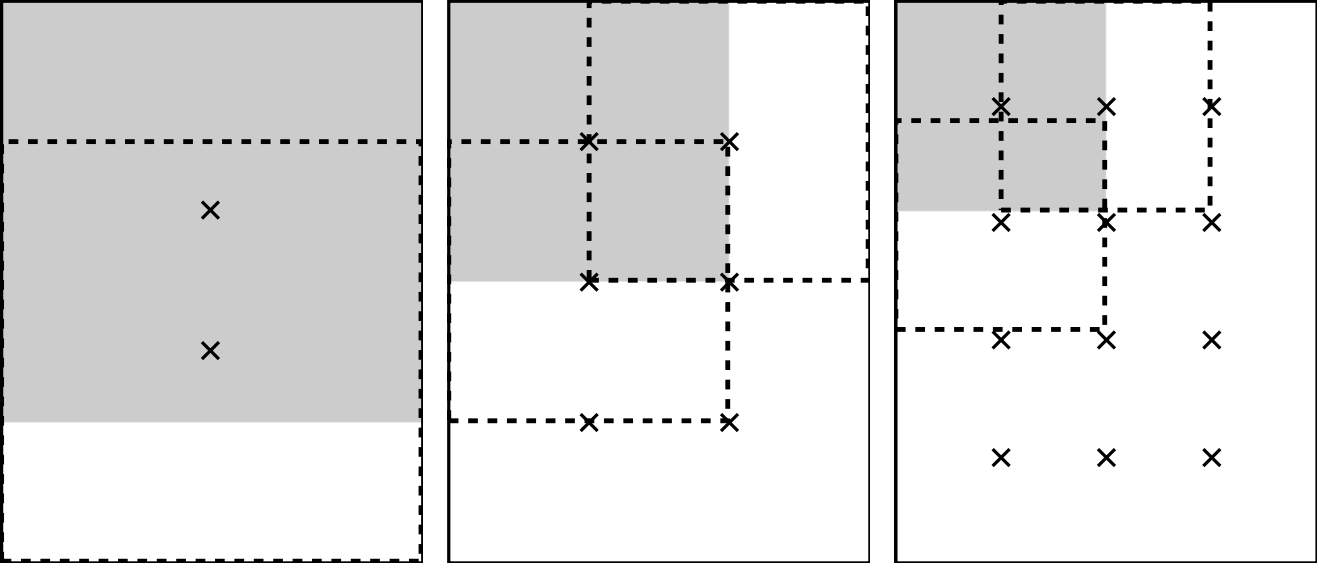
\includegraphics[width=0.6\linewidth]{img/rmac-regions}
    \caption{Example of regions chosen to extract the \gls{rmac} image descriptor from a \gls{cnn} feature map. \figfrom{tolias2016rmac}}
    \label{fig:back:rmac-regions}
\end{figure}

\paragraph{Learning Representations for Retrieval}
Representations obtained by transfer learning and their aggregation demonstrated the potential of features extracted by \glspl{cnn}.
Succeeding work further improved the state of the art by learning directly for the task of instance image retrieval.
% Babenko et al (2014): classif loss
% (Gordo et al, 2016): pretrained models finetuned for retrieval?
% (Radenovic et al, 2016): pretrained models finetuned for retrieval?
% \cite{arandjelovic2016netvlad}: NetVLAD

% FROM Gordo: A preliminary version of our work (Gordo et al, 2016), together with a concurrent work (Radenovic et al, 2016), confirmed that finetuning the pretrained models for retrieval can bring a significant improvement, but demonstrated that even more crucial are the combination of i) a good image representation and ii) a ranking loss – as opposed to the classification loss used by Babenko et al (2014).
% From Gordo RMAC+: Here, we argue that one of the main reasons that prevented previous retrieval methods based on deep architectures to perform well is their lack of supervised learning for the specific task of instance-level image retrieval~\cite{radenovic2016cnn,gordo2017end}. In this work, we focus on the problem of learning representations that are well suited for the retrieval task.
%The recent NetVLAD~\cite{arandjelovic2016netvlad} also highlights the importance of learning to rank.

% RMAC+
\subsection{Cross-modal Image Retrieval}
%Cross-modal Retrieval
%Textual / visual / common space retrievals


\subsection{Evaluation Metrics}
The image retrieval problem is not so different from classical textual information retrieval problem, thus it borrows from it much of the terminology, formulations and evaluation metrics.
% accuracy, computational cost, memory consumption
The main aspects to be considered in the evaluation of a retrieval system are its accuracy and its computational \& memory consumption in both the off-line and on-line stages.
While measuring computational and memory resources in this scenario is straightforward, researches dedicated multiple metrics to measure the accuracy of a retrieval system.
In the following paragraphs, we will introduce the notation and some of the conventionally used evaluation metrics.

Given a collection of images $\X$ and a query image $\q$, the goal is to retrieve the set of images $\X_q \subset \X$ relevant to $\q$.
In the feature-based approach, an image is represented by its feature vector $\x$, and a similarity $s(\cdot)$ (or distance $d(\cdot)$) function is defined to compare two feature vectors.
This function permits to assign a similarity score (or a distance) to each element of our search collection and to sort them based on their relevancy to the query.
Since the top elements on the candidate list are the ones to be most plausible to be consumed by the user, many of the evaluation metrics for measuring the accuracy of a retrieval system are thought to evaluate the goodness of the initial part of the results list.

Assume $\X$ %$= {\x_1, \ldots, \x_N}$
is a collection of $N$ elements, $\q$ a query, $\Y^{\star}_{\q} \subset \X$ the subset of $\X$ relevant to $\q$, and $\Y_{\q}$ the retrieved candidate set to be evaluated.
% = {\y_1, \ldots, \y_N} \subset \{0,1\}^N$ a set of $N$ indicator variables where $\y_i = 1$ if $\x_i$ is relevant for $\q$, 0 otherwise.
% PR
\paragraph{Precision and Recall}
With \emph{precision}, we refer to the fraction of retrieved samples that are relevant to the query
\begin{equation} \label{eq:back:precision}
\mathrm{Precision} = \frac{|\Y_{\q} \cap \Y^{\star}_{\q}|}{|\Y_{\q}|} \,,
\end{equation}
where $|\cdot|$ indicates the cardinality of a set.
We refer to the fraction of relevant samples actually retrieved as \emph{recall}
\begin{equation} \label{eq:back:recall}
\mathrm{Recall} = \frac{|\Y_{\q} \cap \Y^{\star}_{\q}|}{|\Y^{\star}_{\q}|} \,.
\end{equation}

A trade-off between precision and recall is often tuned on deployment;
the system may be tuned to retrieve only objects similar to the query with high confidence thus achieving high precision, but may leave behind some relevant samples and obtaining a low recall.
Viceversa, a less stringent retrieval has a high recall, but more retrieved samples may not be relevant to the query, decreasing the precision of the system.

% mAP
\paragraph{\acrlong{ap}}
The \emph{\acrfull{ap}} metric is commonly used to evaluate a retrieval system independently from the particular configuration of precision-recall.
Similarly to the \acrfull{auc} of ROC plots -- discussed in \ref{subsec:back:classif-eval} -- the \gls{ap} represent the area under the precision-recall curve and is computed as
\begin{equation} \label{eq:back:ap}
    \mathrm{AP} = \sum_r p(r)\,,
\end{equation}
where $r$ is the set of possible recall values that can be achieved, e.g. varying the maximum number of elements to be retrieved or the threshold on the scores of the retrieved samples.
When multiple queries are considered for evaluation, the \emph{\acrfull{map}} is usually reported, which is the mean of the \glspl{ap} obtained from each query.

%nDCG
\paragraph{\acrlong{dcg}}
The \emph{\acrfull{dcg}}~\cite{jarvelin2002cumulated} is conventionally used when multiple level of relevancy are available for samples in the groundtruth.
Its aim is to penalize highly relevant samples in the bottom part of the results;
to do so, usually a logarithmic weighting scheme is adopted to assign a decreasing importance to samples in the lower part of the search results.
The \gls{dcg} at the rank position $n$ is defined as
\begin{equation} \label{eq:back:dcg}
    \mathrm{DCG}@n = \sum_{i=1}^n \frac{2^{r_i} - 1}{\log_2(i + 1)} \,,
\end{equation}
where $r_i$ is a positive scalar representing the relevance of the $i$-th retrieved sample.
In the case rankings can have ties, the \gls{tdcg}~\cite{mcsherry2008computing} is used, defined as:
%
\begin{equation}
\mathrm{TDCG}@n = \sum_{i=1}^{m}\left(\left(\frac{1}{n_i}\sum_{j=t_i+1}^{t_{i+1}}2^{rel_i}-1\right)\sum_{j=t_i+1}^{\min(t_{i+1},k)}\frac{1}{\log_2(i+1)}\right)
\end{equation}
%
where $m$ is the number of group of ties in the ranking of the first $n$ results, $n_i$ indicates the number of tied result in the $i$-th group, $t_i$ indicates the starting position of each tied group.
The $TDCG$ is derived from $DCG$ by observing that the average gain for a position in a group of tied results is the average of the gain of such tied results.
The $TDCG$ is obviously equivalent to $DCG$ in the case there are no ties in the results.

% NDCG is divided by a normalization factor to ensure the metric is in the $[0,1]$ range.

% R@K
\paragraph{\acrlong{r@k}}
The \acrfull{r@k} is the recall metric when considering only the top-K results of the groundtruth as relevant.
It is conventionally used to compare two rankings in absence of an explicit relevancy labelling of the groundtruth.
Assuming $\Y^{\star}_{\q, K}$ the set of samples relevant to $\q$ truncated at the $K$-th element, and $\Y_{\q,K}$ the top-$K$ retrieved elements to be evaluated, the \gls{r@k} is defined as
\begin{equation} \label{eq:back:r@k}
    R@K = \frac{|\Y^{\star}_{\q, K} \cap \Y_{\q,K}|}{K} \,.
\end{equation}

%medR
\paragraph{\acrlong{medR} and \acrlong{mrr}}
These metrics are particularly useful when evaluating rankings in which there is only one object in the database relevant to the query that need to be retrieved.
Cross-modal retrieval with coupled datasets is an examples in which this condition applies: using as query one modality of a sample, a common approach is to evaluate how well the system is able to retrieve the same sample in the different modality.
Given multiple queries, the \acrfull{medR} is the median of the positions of the relevant objects in the rankings, one per query,
% MRR
while the \acrfull{mrr} is the mean of the reciprocals of the same quantities.


\subsection{Image Indexing}
%\label{sec:back:indexing}
%kNN schemes
%Permutation-based representations
%Deep Permutations

%Datasets & Evaluation Metrics

\section{Datasets}
\label{sec:back:datasets}
In this section, we will list the dataset -- either publicly available or collected -- used directly or indirectly in the experiments presented in this work.

\subsection{Classification Datasets}

\paragraph{\acrfull{ilsvrc} 2012~~\cite{russakovsky2015imagenet}}
The \acrfull{ilsvrc} 2012 dataset is composed by a large set of images of general objects collected for evaluating algorithms for large-scale visual object recognition.
It is a subset of roughly 1.3 million images taken from the larger ImageNet\footnote{\url{http://www.image-net.org}} database -- a big collection of images labelled and organized following the hierarchical categorization of WordNet.
Images are assigned a single label chosen from the 1,000 classes selected for the competition, spanning general objects, animals, etc.
Each class has roughly 1,000 images in the training set (the number oscillates between 700 and 1,300), and exactly 50 and 100 images respectively in the validation and test set, for a total of 1,281,167 images for the train set, 50,000 for the validation set, and 100,000 in the test set.
Only the training and validation sets are publicly available.

\paragraph{Places205~\cite{zhou2014learning}}
The Places205 dataset is composed by roughly 2.5 million images collected from image search engines labelled with 205 semantic scene categories and attributes representing visual environments all over the world.
It is a subset of the bigger Places dataset~\cite{zhou2016places}.

\paragraph{PKLot~\cite{de2015pklot}}
The PKLot dataset is an car parking occupancy detection dataset comprised by 12,417 images of 3 parking lots, named UFPR04, UFPR05, and PUC, took in different days and weather conditions.
The images have been segmented in 695,899 images of parking spaces by cropping along the rotated rectangles delimiting each parking space and rotating back the cropped patches in vertical or horizontal position.
Each segmented image is labelled with the vacancy status of the slot, which can be either occupied or vacant.

\paragraph{CNRPark+EXT~\cite{amato2016car,amato2017deep}}
The CNRPark+EXT dataset is a car parking occupancy detection dataset collected during this thesis from the parking lots of the campus of the National Research Council (CNR) in Pisa.
It is comprised by roughly 150,000 images of parking spaces taken from 9 smart cameras with different view-points, in different days with different weather and light conditions, and includes occlusion and shadow situations that make the occupancy detection task challenging.
More details about the CNRPark-EXT dataset will
be given in \ref{ch:deep-parking}.

\paragraph{Twitter Testing Dataset~\cite{you2015robust}}
The Twitter Testing Dataset is a dataset for image sentiment analysis composed by 1269 images labelled with crowd-sourcing (Amazon Mechanical Turk) following a binary positive/negative sentiment polarity scheme.
Each image has been annotated as positive or negative by five workers, and three different subsets have been created, respectively comprised by images where 5 workers agree on the sentiment of the image (5-agree, 882 images), where at least 4 workers agree (4-agree, 1,116 images), and where at least 3 workers agree (3-agree, whole set of images).

\paragraph{\acrfull{t4sa}~\cite{vadicamo2017cross}}
The \acrlong{t4sa} dataset is a large-scale weakly-labelled dataset for sentiment analysis collected during this thesis to evaluate the weakly-labelled cross-media training procedure for image classifiers presented in \ref{ch:weakly-labelled}.
It is comprised by 904,395 tweets and their corresponding 1,473,394 images (each tweet has one or more images);
tweets have been collected from the 5\% random stream of global tweets provided by the Twitter APIs keeping only tweets in english with at least five words and at least one image.
Each tweet is associated with a three-way sentiment polarity (positive/neutral/negative sentiment) predicted by performing textual sentiment polarity prediction.
More details are available in \ref{ch:weakly-labelled}.

\subsection{Retrieval Datasets}

\paragraph{INRIA Holidays~\cite{jegou2008hamming}}

The INRIA Holidays image set is an image retrieval dataset comprised by 1491 high-resolution holidays photos containing various scenes types.
The authors chose 500 queries and manually selected from the set the images relevant for each query.
A frequently used variant of this dataset is the one augmented with \emph{MIRFlickr1M}, a distractor set of 1 million images collected by the Flickr service;
we refer to this new dataset as \emph{Holidays-MIRFlickr1M}.

\paragraph{Oxford Buildings~\cite{philbin2007object}}
The Oxford Buildings dataset, also known as \emph{Oxford5k}, is an image retrieval dataset comprised by 5,062 images of various buildings present in Oxford.
The set is composed by photos of 11 famous buildings plus distractor images collected from Flickr.
For each building, five queries are specified with bounding boxes delimiting the building we are interested in retrieving, for a total of 55 query images.
For each query, images of the search set are assegned with one of the following four labels:
\begin{itemize}
    \item \emph{ok} -- if the image contains a clear look of the building in the query;
    \item \emph{good} -- if more than 25\% of the building is clearly visible;
    \item \emph{junk} -- if less than 25\% of the building
is visible, or there is a very high level of occlusion or dis-
tortion;
    \item \emph{absent} -- if the building is not present.
\end{itemize}
In this work, we will adopt the version of this dataset augmented with a distractor set of 100k images collected from Flickr, and we will refer to it as \emph{Oxford-Flickr100k}.

% \paragraph{Paris~\cite{philbin2008lost}}
% \paragraph{Flickr100k and Flickr1M ~\cite{philbin2007object}}

\paragraph{\acrfull{coco}~\cite{lin2014microsoft}}

The Microsoft \acrfull{coco} dataset is a collection of images  for large-scale object detection, segmentation, and captioning.
it is comprised by 2,500,000 labeled object instances belonging to 91 common object categories in 328,000 images.
Each image is associated with an instance-level pixel-wise segmentation of the object instances it depicts and five captions describing the whole images.
This dataset is particularly adopted also in cross-modal retrieval due to its large scale and the presence of captions, and we will use it to compare to existing cross-modal retrieval approaches in \ref{ch:text-to-vis}.

\subsection{Others}

\paragraph{NIPS Adversarial Attacks and Defences Competition DEV set~\cite{kurakin2018adversarial}}
The NIPS Adversarial Attacks and Defences Competition DEV set is comprised by 1,000 images that do not belong to the \gls{ilsvrc}'12 subsets but share the same label space, i.e. are labelled with one of the same 1,000 label used in \gls{ilsvrc}.
This set has been released in the context of the NIPS Adversarial Attacks and Defences Competition on Kaggle to let participants work with pre-trained \gls{ilsvrc} classifiers using images not involved in their training process.
In particular, the set is devoted to generate adversarial examples for image classifiers, i.e. maliciously manipulated images the lead a classifier to misbehave.
More details are available in \ref{ch:detect-advesarial} in which we use this set of images to evaluate a detection scheme for adversarial attacks.

%======================= MINIATURIZE CNN FOR EMBEDDING ===========================

%TODO uniforma view-point viewpoint
%TODO uniforma \emph{AlexNet} e AlexNet
%TODO captions

\graphicspath{{img/parking/}}

\chapter{Miniaturization of Convolutional Neural Networks for Embedded Devices}
\label{ch:miniaturization}

One of the most important limitations of \glspl{dcnn} is that they often rely on computationally expensive deep models, which are slow for many applications including image classification.
Due to this limitation, methods based on efficient hand-crafted local features --- such as \acrshort{surf}, \acrshort{orb}, \acrshort{lbp}, etc.\ --- are predominantly adopted in vision systems where a computational power of a full-featured server is not available, e.g.\ mobile phones or embedded devices.

In this chapter, we will explore the adoption and the miniaturization of \glspl{dcnn} for efficient image classification.
We focus our investigation on reducing and evaluating deep models for embedded vision systems, i.e.\ smart cameras.
A smart camera is an embedded camera equipped with a limited computational and communication capabilities that can be used to process, extract, and send information contained in the captured images on board of the device itself.
% TODO [CITE] smart surveillance or campus with CNNs
Empowering smart cameras with the generalization and robustness of \glspl{cnn} for computer vision application represents one the most promising steps towards the evolution of smart environments \cite{}.
Their ``smart'' nature makes them suitable for automated intelligent systems able to generate event descriptions and/or make decisions \cite{belbachir2010smart}, thus making them attractive to a broad range of applications.
In our study, we will focus on a specific application, that is the visual occupancy detection of outdoor car parking lots in a decentralized fashion with smart cameras.
The motivation for the choice of this specific problem is manyfold.
\begin{itemize}
	% easy problem formulation as 2-way classification
	% lack of deep learning solutions for the problem
	\item The problem of visual occupancy detection of parking spaces can be easily formulated as a binary image classification problem;
	this enable us to focus on the engineering aspects about model reduction and its evaluation;
	moreover state-of-the-art approaches tackling this problem are based on hand-craft features and shallow machine learning, while a deep learning solution could (and will) bring an improvement of the detection accuracy and robustness.

	% current systems vision solutions are centralized, with BW costs
	\item Parking lot occupancy detection systems are commonly implemented by means of expensive magnetic ground sensors, while vision-based systems provide a more cost-effective solution;
	in our setup, a single smart camera can simultaneously monitor up to 50 parking slots at a cost significantly lower than the one required to install and maintain ground sensors for every slot.

	% decentralize for flexibility and bw cost
	\item In centralized solutions, ``dumb'' cameras send their video feeds to a server which process them;
	a decentralized solution instead brings a reduction of the communication overhead and the elimination of the computing bottleneck, thus increasing even further the scalability of the solution;
	moreover, an intelligent infrastructure provides flexibility in its application, e.g.\ the same cameras could be used for perimeter surveillance during night hours.

\end{itemize}

While visual approaches to parking lot occupancy detection are not new \cite{dan2002parking,wu2007robust,del2015vacant,de2015pklot}, the usage of solely visual information still poses challenges in terms of robustness.
Numerous solutions are tailored to specific scenarios and hardly generalize well to different ones, such as a different parking lot, view-point, light conditions, or occlusion patterns.

In our investigation, we propose a decentralized and efficient vision system based on smart cameras and \gls{dl} for parking lot occupancy detection.
We present a reduced \gls{dcnn} suitable for embedded devices with which we implement the classification logic under the occupancy detection task.
A strong experimental protocol on publicly available datasets is applied to compare the proposed approach to the state-of-the-art methods and deep models and assess the its generalization properties.
In addition, we contribute with a publicly available dataset of the parking lot images captured by multiple cameras called \emph{CNRPark-EXT} that enables us to thoroughly test the robustness of our solution to multiple source of errors.

The chapter is organized as follows.
In \ref{sec:mini:related-work}, we introduce the work related to parking lot occupancy detection, focusing on vision-based solutions more related to our proposal.
In \ref{sec:mini:occupancy-detection}, we propose and describe the \gls{dcnn} model specifically designed to be executed on smart cameras which implements the parking slot classification pipeline.
In \ref{sec:mini:datasets}, we presents the already available and newly collected datasets used to evaluate and compare our approach.
\ref{sec:mini:evaluation} presents the proposed experimental setup to compare the our approach to the state of the art and evaluate its robustenss to multiple aspects.
\ref{sec:mini:deployment} briefly describes the deployment of our solution in a real scenario and gives an overview of the overall system.

The research presented in this chapter was published in~\cite{amato2016car,amato2017deep}, and the provided resources --- e.g.\ datasets and trained models --- are available at \url{http://cnrpark.it}.

\section{Visual Occupancy Detection and Related Work}
\label{sec:mini:related-work}

Techniques for car parking occupancy detection are of great importance for an effective management of car parking lots.
Knowing in real-time the availability of free parking spaces and communicating it to the users can be of great help in reducing the queues, traffic jams, and the time required to find an available parking slot.
In the following paragraphs, we will review some of the work targeting this problem, focusing on vision-based methods.

\paragraph{\gls{ml}-based approaches}
% Occupancy Detection w/o CNNs
Many attempts before the \gls{dl} era were implemented by classical \gls{ml} methods applied on hand-crafted visual features.
\citet{dan2002parking}, one of earliest work using this approach on the subject, used \glspl{svm} on color features to classify regions of the parking lot as `car` or `empty-space`.
Among the challenges arose by the task, the problem of occlusions due to obstacles or camera angle is one of the most significant.
\citet{wu2007robust} tried to overcome occlusion by neighboring cars by considering also the neighbor parking slots of the one to be classified.
The \gls{svm} classifier for a slot is defined over the colour features computed across three slots (the slot itself and the two neighbor slots).
\citet{tsai2007vehicle} used multiple hand-crafted features and a Bayesian classifier to deal with the problem of light changes, while
\citet{huang2013vacant} employed a Bayesian hierarchical framework based on a 3D model of the parking spaces.
Similarly, \citet{delibaltov2013parking} proposed a method based on a 3D model of every parking slot in order to account for occlusions when classifying a slot as vacant or occupied.
In~\cite{jermsurawong2014one}, a customized neural networks based on visual features is used to model the occupancy status of slots and the parking demand. % TODO check paper
% they present robust results for night and day classifiers in a one-day long evaluation based on 126 parking spaces.
In~\cite{de2015pklot}, the authors employed ensembles of \gls{svm} classifiers based on multiple textural features --- such as \gls{lbp}, \gls{lpq}, and their variations --- and they present a dataset of roughly 700,000 images of parking spaces coming from three different cameras used in their experiment.
\citet{del2015vacant} proposed a temporal analysis of the video frames based on background subtraction to detect and track parking and leaving vehicles.
In a similar fashion, \citet{masmoudi2014} propose to overcome the occlusion problem by visually tracking cars entering or leaving a parking space.

\paragraph{Non-vision approaches}
In addition to approaches using visual techniques and commercial solutions using ground sensors, there are techniques harnessing sensors installed on cars or carried by the drivers.
In \cite{caicedo2012prediction}, the authors argue that occupancy detection can be solved by interacting with smart in-vehicle navigation systems.
\citet{lan2014intelligent} instead proposed to harness sensors in smart phones and other devices to collect real-time parking availability information.
%
\paragraph{\gls{dl}-based approaches}
To the best of our knowledge, the proposed approach is the first work that employs \glspl{dcnn} in the context of parking lot monitoring.
A relevant work in a similar --- yet different --- task is \cite{chen2014vehicle}, where the authors employed a multi-scale \gls{cnn} to detect vehicles in high-resolution satellite images.

\section{\glspl{dcnn} for Occupancy Detection in Embedded Devices}
\label{sec:mini:occupancy-detection}

\begin{figure}
	% TODO [FIGURE] alex e malex a confronto
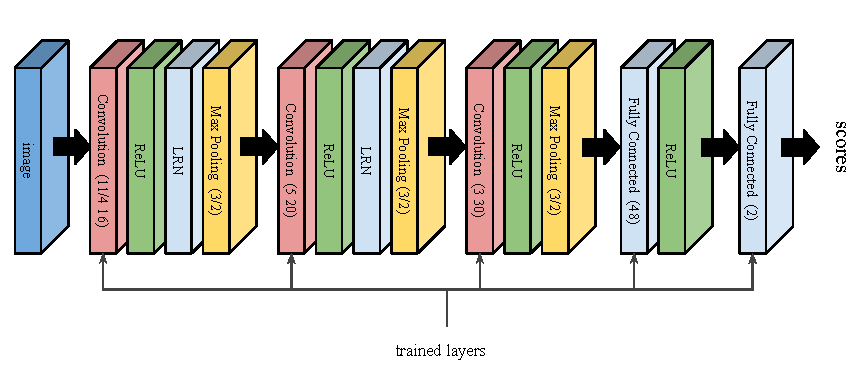
\includegraphics[width=\linewidth]{net-archit}
% 	\newcolumntype{Y}{>{\centering\arraybackslash}X}
% 	\begin{tabularx}{\textwidth}{|Y|Y|Y|Y|Y|Y|}
% 		% \begin{tabular}{|c|c|c|c|c|c|}
% 		\hline
% 		\emph{net} & \emph{conv1} & \emph{conv2} & \emph{conv3} & \emph{fc4} & \emph{fc5} \\ \hline \hline
% %		             & 30x11x11+4     & 20x5x5+1       &                & 100          & 2            \\
% %		mLeNet       & pool 5x5+5     & pool 2x2+2     & -              & ReLU         & soft-max     \\
% %		             & -              & -              &                &              &              \\ \hline \hline
% 		             & 16x11x11+4     & 20x5x5+1       & 30x3x3+1       & 48           & 2            \\
% 		mAlexNet     & pool 3x3+2     & pool 3x3+2     & pool 3x3+2     & ReLU         & soft-max     \\
% 		             & LRN, ReLU      & LRN, ReLU      & ReLU           &              &              \\ \hline
% 	\end{tabularx}
\caption{CNN Architecture: for convolutional layers \emph{conv1-3}, parameters are specified as ``$size/stride~num$''.
For max-pooling, parameters are specified as ``$size/stride$''.
For fully connected layers we report their dimensionality.
The last fully connected layer is followed by a 2-way softmax classifier.}
\label{fig:mini:cnns}
\end{figure}

% \begin{table}

% 	\caption{CNN Architecture: for convolutional layers \emph{conv1-3} the
% 		first row in a cell specifies the number and the size of filters as
% 		``$num \times width \times height + stride$''. The second row specifies
% 		the max-pooling operation applied as ``$width \times height + stride$''.
% 		The third row indicates if Local Response Normalization (LNR) and/or
% 		Rectified Linear Unit (ReLU) activation are applied. For fully connected
% 		layers we report their dimensionality. The last fully connected layer
% 	    is followed by a 2-way soft-max classifier.}
% 	\label{tbl:cnns}
% \end{table}

\noindent The main objective of our proposal is to design a \gls{cnn}-based classifier for the problem of occupancy detection runnable by smart cameras and low-power embedded devices in general.
Due to its popularity and wide-spread adoption, we adopted the Raspberry Pi 2 model B \footnote{\url{https://www.raspberrypi.org/products/raspberry-pi-2-model-b/}} equipped with the standard Raspberry Pi camera module \footnote{{https://www.raspberrypi.org/documentation/hardware/camera.md}} as a reference hardware implementation of a smart camera.

As done in previous work, we formulate the visual occupancy detection of a parking slot as a binary classification problem in which an image of a single parking space is either labelled as \emph{vacant} or \emph{occupied}.
We assume that the cameras are fixed, and each of them monitors several parking slots.
The images of the individual slots are obtained from the entire frame by cropping fixed regions that have been manually defined off-line, and the smart camera is in charge of performing an independent classification for each image.

% TODO [CITE] AlexNet applications
As a starting point for the design of our solution, we considered the very popular \emph{AlexNet} \gls{cnn} for image classification~\cite{krizhevsky2012imagenet}, which is used as reference in many computer vision applications~\cite{}.
Such architecture exploits its massive number of parameters to learn a non-linear mapping from pixels to high-level features that facilitate classification.
However, its computational budget and memory footprint poses severe limitations on devices with limited resources,
especially when taking into account that the number of monitored slots per camera can easily reach 50--100.
Moreover, considering that a forward pass of AlexNet on the Raspberry Pi model B on a 224x224 RGB image takes roughly 20 second while occupying most of the RAM available on the device\footnote{Data collected using the implementation of AlexNet of the Caffe~\cite{jia2014caffe} library}, it is evident that this architecture does not scale to the size of the problem.

We argue that the problem of visual occupancy detection --- despite the presence of high variability factors such as changing light conditions, viewpoints, and occlusion patterns --- is less complex with respect to the \gls{ilsvrc}'12 classification task AlexNet was designed for.
We define a reduced \gls{dcnn} architecture --- named \emph{miniAlexNet} or simply \emph{mAlexNet} --- to implement a simplified classifier, and we compare its performance and computational cost with respect to the original AlexNet.
The architecture of \emph{mAlexNet} follows the AlexNet one.
We keep the dimensionality of the input unaltered, i.e.\ a $224 \times 224$ RGB image, that in our scenario will contain the visual appearence of a single parking slot.
In case of differently-sized images, they are resized to match the input dimensionality.
We reduced the number of convolutional layers from five to three, the first two followed by max-pooling, \gls{lrn}, and \gls{relu} activations, while in the third one, the \gls{lrn} is omitted.
The number of fully-connected layers is reduced to two, including the one producing the final prediction.
We drastically reduced the number of filters and neurons of all layers, starting from the minimalist number of 16 filters in the first convolution layer and defining the dimensionality of subsequent layers following the proportions of the original architecture.
We argue that a small number of convolutional filters in the first layer are sufficient to detect low-level features important for the task --- such as edges and corners with multiple rotations --- while reducing the possibility of overfitting.
We maintained the convolutional kernel sized and pooling sizes of the original architecture, since we share the same image input shape.
The obtained model has roughly 42,000 parameters, that is roughly $1360 \times$ less with respect to AlexNet.
\ref{fig:mini:cnns} reports the details of the proposed architecture.
As confirmed by experiments reported in \ref{sec:mini:evaluation}, using a smaller model for visual occupancy detection does not entail a severe performance degradation.
The Caffe implementation of our model is able to perform on average 50 parking slot classifications on a single Raspberry Pi model B in roughly 15 seconds, which is an acceptable cycle time for parking lot occupancy detection systems. % TODO? note on new impl?
The training phase, which need a considerable amount of computational resources, is performed off-line once on a powerful device, and the final classification model is deployed on multiple smart cameras once it is trained.

\section{Datasets}
\label{sec:mini:datasets}

In this section, we will describe the two datasets used to train and evaluate our proposed parking slot classifier.

\paragraph{PKLot}
The first dataset, PKLot~\cite{de2015pklot}, includes 695,899 images of parking slot extracted from photos of two parking lots --- dubbed UFPR and PUC --- taken by three cameras in multiple weather conditions and spanning different days.
Two cameras captured images of the UFPR parking lot from two different view-points identified by the names UFPR04 and UFPR05, while the other one is dedicated to the PUC lot.
Slot images are obtained from the full camera frame by manual segmentation of non-occluded and non-overlapping spaces: rotated rectangles are placed on the image to precisely identify the slots in each parking lot, and regions are subsequently extracted from frames using the defined mask.
This segmentation strategy results in a precise coverage of the parking slot without strong forms of occlusion.
Extracted patches are then straightened to the nearest vertical or horizontal orientation depending on the orientation of the rotated rectangle used as mask.
Every patch is manually labelled either as `vacant` or `occupied`.

\begin{figure}
\centering
\begin{subfigure}[b]{0.49\columnwidth}
	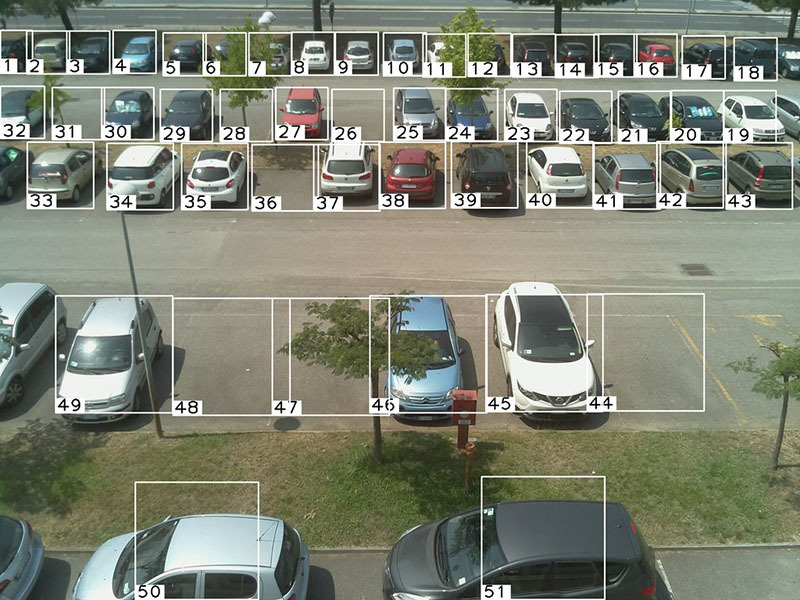
\includegraphics[width=\columnwidth]{camera-a-overview}
	\caption{Overview of CNRPark CAM A}
	\label{fig:mini:cam-a}
\end{subfigure} %
\begin{subfigure}[b]{0.49\columnwidth}
	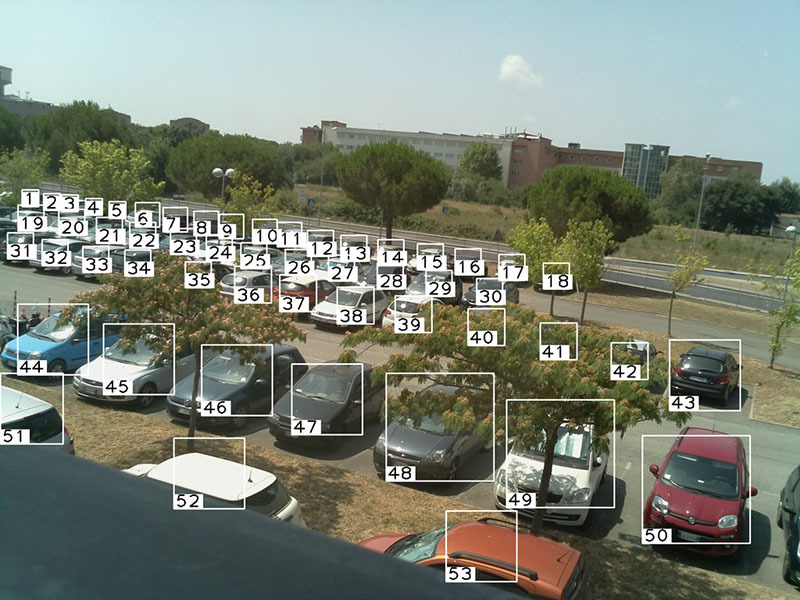
\includegraphics[width=\columnwidth]{camera-b-overview}
	\caption{Overview of CNRPark CAM B}
	\label{fig:mini:cam-b}
\end{subfigure}

\begin{subfigure}[b]{0.49\columnwidth}
	\includegraphics[width=\columnwidth]{overview-cam1}
	\caption{Overview of CNRPark-EXT CAM 1}
	\label{fig:mini:cam-1}
\end{subfigure} %
\begin{subfigure}[b]{0.49\columnwidth}
	\includegraphics[width=\columnwidth]{overview-cam8}
	\caption{Overview of CNRPark-EXT CAM 8}
	\label{fig:mini:cam-8}
\end{subfigure}
\caption{Segmentation masks for parking slot images in the preliminary \emph{CNRPark} dataset (top) and in the extended \emph{CNRPark-EXT} dataset (bottom, only for camera 1 and 8)}
\label{fig:mini:cam-overview}
\end{figure}

\begin{figure}
\begin{subfigure}{0.25\columnwidth}%
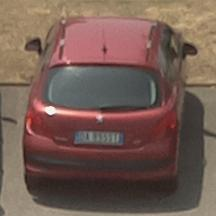
\includegraphics[width=\columnwidth]{38busy}%
\end{subfigure}%
\begin{subfigure}{0.25\columnwidth}%
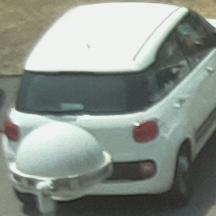
\includegraphics[width=\columnwidth]{34busy}%
\end{subfigure}%
\begin{subfigure}{0.25\columnwidth}%
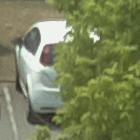
\includegraphics[width=\columnwidth]{11busy}%
\end{subfigure}%
\begin{subfigure}{0.25\columnwidth}%
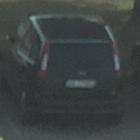
\includegraphics[width=\columnwidth]{13busy}%
\end{subfigure}

\begin{subfigure}{0.25\columnwidth}

\includegraphics[width=\columnwidth]{38empty}%
\end{subfigure}%
\begin{subfigure}{0.25\columnwidth}%
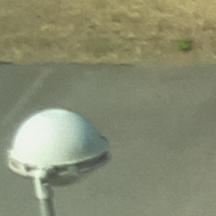
\includegraphics[width=\columnwidth]{34empty}%
\end{subfigure}%
\begin{subfigure}{0.25\columnwidth}%
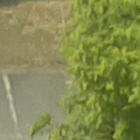
\includegraphics[width=\columnwidth]{11empty}%
\end{subfigure}%
\begin{subfigure}{0.25\columnwidth}%

\includegraphics[width=\columnwidth]{13empty}%
\end{subfigure}
\caption{Example of segmented parking slots images under different light conditions and occlusion patterns.
The first and second rows show four slots respectively in `occupied` and `vacant` state}
\label{fig:mini:slots}
\end{figure}

\paragraph{CNRPark}
In order to measure the generalization power of the proposed approach to unseen scenarios, we personally built a new dataset --- named \emph{CNRPark} --- collecting images from the parking lot in the campus of the National Research Council (CNR) in Pisa.
The preliminary version of this dataset --- which we refer to as CNRPark --- contains roughly $12,000$ images of slots of a part of the parking lot which were collected from 2 Rasperry Pi cameras (denoted as camera $A$ and $B$) with different perspectives and angles of view in different days of July 2015 (see \ref{fig:mini:cam-a,fig:mini:cam-b}).
Images of individual parking slots are extracted using manually-placed squared masks from the full camera frame.
Slot masks are placed to minimize the part of adjacent slots contained in the image, often limiting the area usable for classification to just a part of the entire slot.
Moreover, in many slots, occlusions by adjacent cars and obstacles (e.g.\ trees, lampposts) are inevitable due to the skewed field of view of the cameras;
this also involves that slots images have different sizes depending on the distance of the slot from the capturing camera.
Thus, our dataset poses additional challenges to occupancy detection methods that can be commonly found in real scenarios.
We split the dataset in two non-overlapping sets named \emph{CNRParkOdd} and \emph{CNRParkEven} respectively containing slot images having odd or even slot id.
This permitted us to test the generalization of our approach by training on some slots and test on unseen slots.

\paragraph{CNRPark-EXT}
We subsequently extended the CNRPark dataset gathering more images of the complete parking lot --- comprised by 164 parking slots --- captured by 9 additional cameras from November 2015 to February 2016.
\ref{fig:mini:cam-1,fig:mini:cam-8} report the cameras with respectively the most and least skewed views.
Images were collected in multiple days spanning multiple seasons of the year, and the number of slots monitored by each camera roughly spans from 10 to 50.
To extract the images of individual slots, we followed the same strategy of CNRPark.
The extended version of the dataset --- dubbed \emph{CNRPark-EXT} -- is composed of 4,287 camera frames acquired in 23 different days, from which we obtained 144,965 manually labeled images of individual parking slots.
The added value of our dataset stands in the fact that it captures a variety of occlusion and shadow patterns, and light and weather conditions (see \ref{fig:mini:slots}) that cover more real-case scenarios with respect to existing datasets.
Slot images are grouped by camera ID, by time of capture, and by three weather conditions --- i.e.\ \emph{Sunny}, \emph{Overcast}, and \emph{Rainy}.
We also provide splits for training, validation, and test sets;
we ensured that images captured in a particular day do not span more than one set.

\ref{tab:mini:datasets} reports detailed information about the composition of \emph{CNRPark}, \emph{CNRPark-EXT}, and \emph{PKLot}~\cite{de2015pklot}.
The main difference between our datasets and the existing ones can be summarized as follows.
Slot images in \emph{CNRPark-EXT} often do not cover precisely or entirely the parking slot volume, whereas in \emph{PKLot} slots are registered and straightened, resulting in a more precise coverage of the parking slot.
Moreover, \emph{CNRPark-EXT} captures heavily occlusion patterns (some slots are almost entirely covered by trees and lampposts) and lower point of views, resulting in considerable occlusions due to adjacent vehicles.
Even if our dataset counts less images than \emph{PKLot} and has been collected from a single parking lot, we assessed through experiments that the real challenge comes from the variety of view-points and occlusions patterns of which our dataset is rich:
in fact, we let the \gls{cnn} to cope with these factors, resulting in a more robust classifiers in real case scenarios and in a reduced manual setup effort.

\begin{table}
\newcolumntype{R}{>{\raggedleft\arraybackslash}X}
% \def\arraystretch{1}
\begin{tabularx}{\linewidth}{lRRR}
\toprule
\textsc{Dataset}    & \textsc{vacant} & \textsc{occupied} & \textsc{total} \\
\midrule
%                       &               &               &                \\
%    CNRPark $A$       & 2549          & 3622          & 6171           \\
%    CNRPark $B$       & 1632          & 4781          & 6413           \\ \hline
%    CNRPark           & 4181          & 8403          & 12584          \\

     CNRPark           & 4,181          & 8,403          & 12,584          \\
     CNRPark-EXT       & 65,658         & 79,307         & 144,965         \\
     PKLot             & 337,780        & 358,119        & 695,899         \\ %\hline
%                       &               &               &                \\
%    CNRPark TRAIN     & 2201          & 3970          & 10000          \\
%    CNRPark VAL       & 1980          & 4433          & 2584           \\ \hline
%    CNRPark           & 4181          & 8403          & 12584          \\
\bottomrule
                       &               &               &                \\
\toprule
\textsc{Subset} & \textsc{vacant} & \textsc{occupied} & \textsc{total} \\ \midrule
    CNRParkOdd        & 2,201          & 3,970          & 6,171           \\
    CNRParkEven       & 1,980          & 4,433          & 6,413           \\ %hline
\midrule
     CNRPark-EXT TRAIN     & 46,877         & 47,616         & 94,493          \\
     CNRPark-EXT VAL       & 5,232          & 13,415         & 18,647          \\
     CNRPark-EXT TEST      & 13,549         & 18,276         & 31,825          \\ %\hline
%     CNRPark-EXT           & 65658         & 79307         & 144965         \\
\midrule
     CNRPark-EXT SUNNY     & 25,665         & 37,513         & 63,178          \\
     CNRPark-EXT OVCST     & 21,067         & 23,176         & 44,243          \\
     CNRPark-EXT RAINY     & 18,926         & 18,618         & 37,544          \\ %\hline
%     CNRPark-EXT           & 65658         & 79307         & 144965         \\
\midrule
     CNRPark-EXT \emph{C1}      & 6,407          & 9,308          & 15,715          \\
     CNRPark-EXT \emph{C2}       & 1,454          & 2,641          & 4,095           \\
     CNRPark-EXT \emph{C3}       & 4,101          & 5,370          & 9,471           \\
     CNRPark-EXT \emph{C4}       & 7,219          & 9,357          & 16,576          \\
     CNRPark-EXT \emph{C5}       & 9,582          & 11,256         & 20,838          \\
     CNRPark-EXT \emph{C6}       & 9,462          & 10,646         & 20,108          \\
     CNRPark-EXT \emph{C7}       & 10,595         & 10,519         & 21,114          \\
     CNRPark-EXT \emph{C8}       & 11,237         & 12,847         & 24,084          \\
     CNRPark-EXT \emph{C9}       & 5,601          & 7,363          & 12,964          \\ %\hline
%     CNRPark-EXT           & 65658         & 79307         & 144965         \\
\midrule
%					   &               &               &                \\
     PKLot2Days        & 27,314         & 41,744         & 69,058          \\
     PKLotNot2Days     & 310,466        & 316,375        & 626,841         \\ %\hline
%     PKLot             & 337780        & 358119        & 695899         \\
%                       &               &               &                \\
\midrule
     PKLot UFPR04 TRAIN& 25,894         & 23,266         & 49,160          \\
     PKLot UFPR04 TEST & 33,824         & 22,859         & 56,683          \\
     PKLot UFPR05 TRAIN& 45,759         & 48,196         & 93,955          \\
     PKLot UFPR05 TEST & 22,600         & 49,230         & 71,830          \\
     PKLot PUC TRAIN   & 114,424        & 106,334        & 220,758         \\
     PKLot PUC TEST    & 115,616        & 87,895         & 203,511         \\ %\hline
%     PKLot             & 337780        & 358119        & 695899         \\
%                       &               &               &                \\
\midrule
     PKLot TRAIN       & 27,314         & 41,744         & 105,843         \\
     PKLot VAL         & 54,909         & 47,453         & 165,785         \\
     PKLot TEST        & 275,894        & 248,583        & 424,269         \\ %\hline
%     PKLot             & 337780        & 358119        & 695899         \\
\bottomrule
  \end{tabularx}
\caption{Details of datasets used in the experiments, with the various proposed subsets.
Values refer to the number of slot images contained in every dataset or subset}
\label{tab:mini:datasets}
\end{table}

\section{Evaluation}
\label{sec:mini:evaluation}

In this section, we present the experimental evaluation and discuss the obtained results.
Our investigation focused on getting insight on three main aspects of the proposed solution that can be summarized by the following questions:
\begin{enumerate}
\item How does our reduced classifier compare against state-of-the-art approaches?
\item How much the generalization performance degrades when using our reduced model instead of the original AlexNet architecture?
\item How much the proposed solution for visual occupancy detection is robust to weather and viewpoint changes?
\end{enumerate}

To answer these question, we extensively evaluated our approach using the two datasets described in \ref{sec:mini:datasets}, i.e.\ PKLot and CNRPark-EXT.
We performed experiments by splitting the datasets into several subsets that we will described in the following subsections.
Details about data splits are summarized in \ref{tab:mini:datasets}.
The usage of multiple methods on multiple datasets also permits us to compare the quality of our newly collected dataset for learning to detect occupancy detection robustly in real scenarios.

% -----

\subsection{Comparison with the State of the Art}
\label{sub:mini:sota}

We compared \emph{mAlexNet} against the state-of-the-art visual occupancy detection system proposed by \citet{de2015pklot}, which is based on \glspl{svm} classifiers with RBF kernels defined over hand-crafted textural features.
Specifically, histograms of \gls{lbp}, \gls{lpq} features and their variations \cite{ojala2002multiresolution, ojansivu2008blur, rahtu2012local} have been tested as input features of the \gls{svm}.
\Glspl{svm} are calibrated to output the probability of a slot to be occupied.
The authors also shown that the performance of the classification can be improved by using ensembles of \gls{svm} classifiers each defined on a particular textural feature:
probability values are fused using simple aggregation functions, such as \emph{Max} and \emph{Mean}, to obtain the final decision for an image slot.

We follow the experimental protocol described in \cite{de2015pklot}.
We split images from each camera of the PKLot dataset (UFPR04, UFPR05, and PUC) into a training and test set with roughly a 50\%--50\% proportion;
for a fair evaluation, we ensure that images collected in a particular day do not appear in both training and test set.
We then train both mAlexNet and the \glspl{svm} on each of the three training set, and tested on all the available test sets.
%
%Similarly, we also repeated the same protocol with our preliminary CNRPark dataset.
%We split CNRPark into two subsets --- CNRParkEven and CNRParkOdd --- respectively containing images of slots having even and odd IDs.
%We train both \glspl{svm} and mAlexNet on one subset and test on the other, and vice-versa.

For each experiment, we evaluated the prediction obtained for the test set by measuring the percentage error (\textbf{Err. \%}), defined as $100 \cdot (1 - \text{Accuracy})$, and the \gls{roc} \textbf{\gls{auc}}.
The former gives us an overall evaluation of the systems assuming a slot is occupied if the probability is above $0.5$, while the latter summarize the behaviour of the systems independently from the probability threshold chosen.


\paragraph{Training and implementation details for mAlexNet}
Input images are squashed to a resolution of $256\times256$ before being fed to the network.
During the training phase, we perform data augmentation by taking a $224\times224$ random crop of the resized image and flipping it horizontally with $\sfrac{1}{2}$ probability.
In the test phase, images are resized to $224\times224$ resolution and no flipping is performed.
All the mAlexNet models are trained with \gls{sgd} with momentum for 18 epochs, with a learning rate of $0.01$ halved every 6 epochs, a batch size of $64$, a momentum of $0.9$, and a weight decay of $5e^{-4}$;
due to the low model complexity, no dropout regularization is used.
To avoid overfit on the test set, we validate our models at each training epoch by evaluating it on a validation set.
As validation sets, we used the training splits of the PKLot cameras --- e.g.\ when testing on PUC test subset, we use PUC training subset as validation set.
We choose as final model for a particular dataset the one which performs best on the validation test.

\paragraph{Training and implementation details for \glspl{svm}}
To train the \glspl{svm}, we employ the procedure and the hyper-parameters as described by \citet{de2015pklot} here summarized.
We extract LBP-type features with a radius of 1 and 8 neighbors.
LPQ features are extracted using window size of 3x3.
The $C$ and $\gamma$ parameters of \glspl{svm} are chosen with grid search and a 5-fold cross-validation on the training set.
We choose the parameters $(C,\gamma)$ obtaining the best 5-fold accuracy, i.e.\ the best accuracy obtained classifying each fold of the dataset with the model trained on the other folds.
The final SVM is then trained on the entire training set using the chosen parameters, and evaluated on the test set.
We followed the same strategy used in \cite{de2015pklot} to obtain a probabilistic score from the output of the \gls{svm}, which evaluates the posterior probability fitting a sigmoid function with two parameters \cite{platt1999probabilistic}.

\begin{table}
    \newcolumntype{C}{>{\centering\arraybackslash}X}
    \begin{tabularx}{\linewidth}{lcX}
        \toprule
        \textsc{Method} & \textsc{Input Dim.}     & \textsc{Input Description} \\
        \midrule
        mAlexNet         & $224\times 224\times 3$ & a 224x224 RGB image \\
        SVM + LBP        & $256$                     & histograms of classical \acrfull{lbp} \cite{ojala2002multiresolution} \\
        SVM + LBPu       & $59$                      & histograms of uniform LBP \cite{ojala2002multiresolution} \\
        SVM + LBPri      & $36$                      & histograms of rotational invariant LBP \cite{ojala2002multiresolution}  \\
        SVM + LBPuri     & $10$                      & histograms of uniform and rotational invariant LBP \cite{ojala2002multiresolution} \\
        SVM + LPQu       & $256$                     & histograms of \acrfull{lpq} (uniform initialization) \cite{ojansivu2008blur} \\
        SVM + LPQg       & $256$                     & histograms of LPQ (gaussian initialization) \cite{rahtu2012local} \\
        SVM + LPQgd      & $256$                     & histograms of LPQ (gaussian derivative initialization) \cite{rahtu2012local} \\
        \bottomrule
     \end{tabularx}
     \caption{Summary of state-of-the-art methods compared against our approach for parking slot occupancy detection}
     \label{tab:mini:methods}
\end{table}

\begin{table}
	\newcolumntype{R}{>{\raggedleft\arraybackslash}X}

	\begin{tabularx}{\linewidth}{lRRRRRR}
	\toprule
	\textsc{Method}               & \multicolumn{2}{c}{\textsc{UFPR04}} & \multicolumn{2}{c}{\textsc{UFPR05}}  & \multicolumn{2}{c}{\textsc{PUC}}  \\
								    \cmidrule(lr){2-3}  \cmidrule(lr){4-5}   \cmidrule(lr){6-7}
	\textbf{Train on UFPR04}      & \textbf{Err. \%} & \textbf{AUC} & \textbf{Err. \%} & \textbf{AUC} & \textbf{Err. \%} & \textbf{AUC} \\
	\midrule
	mAlexNet                      & 0.46 & 0.99      & 6.71  & 0.99    & 1.73  & 0.99 \\
	LPQu / LPQg / LPQg*           & 0.45 & 0.99      & 15.08 & 0.94    & 15.75 & 0.94 \\
	Mean / Max / Max Ensemble*    & 0.36 & 0.99      & 11.67 & 0.95    & 11.60 & 0.95 \\
	\midrule
	\textbf{Train on UFPR05}      & \textbf{Err. \%} & \textbf{AUC} & \textbf{Err. \%} & \textbf{AUC} & \textbf{Err. \%} & \textbf{AUC} \\
	\midrule
	mAlexNet                      &  6.31 & 0.98     & 0.51 & 0.99     & 7.28  & 0.98 \\
	LPQgd / LPQu / LPQu*          & 14.24 & 0.93     & 1.10 & 0.99     & 12.26 & 0.94 \\
	Mean  Ensemble*               & 14.47 & 0.95     & 0.70 & 0.99     & 10.17 & 0.97 \\
	\midrule
	\textbf{Train on PUC}         & \textbf{Err. \%} & \textbf{AUC} & \textbf{Err. \%} & \textbf{AUC} & \textbf{Err. \%} & \textbf{AUC} \\
	\midrule
	mAlexNet                      &  1.97 & 0.99     & 4.00  & 0.99    & 0.10 & 0.99 \\
	LPQg / LBPri / LPQu*          & 12.85 & 0.94     & 17.22 & 0.91    & 0.42 & 0.99 \\
	Mean  Ensemble*               & 11.12 & 0.95     & 15.80 & 0.91    & 0.39 & 0.99 \\
	\bottomrule
	\end{tabularx}

%	\begin{tabularx}{\linewidth}{XRRRR}
%	\toprule
%	                              & \multicolumn{2}{c}{\textsc{CNRParkEven}} & \multicolumn{2}{c}{\textsc{CNRParkOdd}} \\
%	\textsc{Method}               & \multicolumn{2}{c}{\textbf{\small Train on CNRParkOdd}} & \multicolumn{2}{c}{\textbf{\small Train on CNRParkEven}} \\
%									\cmidrule(lr){2-3}                         \cmidrule(lr){4-5}
%								  & \textbf{Err. \%} & \textbf{AUC} & \textbf{Err. \%} & \textbf{AUC} \\
%	\midrule
%	mAlexNet                      & 9.87 & 0.94 & 9.29 & 0.92  \\
%	LPQgd / LBP*                  & 12.35 & 0.95 & 12.79 & 0.92 \\
%	\bottomrule
%	\end{tabularx}

	\caption{Comparison of \emph{mAlexNet} against state-of-the-art approaches presented by \citet{de2015pklot}}
	\label{tab:mini:net-vs-svms}
\end{table}

A summary of the compared methods is reported in \ref{tab:mini:methods}, and results are reported in \ref{tab:mini:net-vs-svms}.
For simplicity, we report for each experiment only the variant of LBP or LPQ that yielded the best performance on each subset, and for ensembles, we report instead the best aggregation function.
We can notice that \emph{mAlexNet} generally perform better then other compared methods in terms of both percentage error and AUC.
All the methods perform well when training and test images comes from the same camera;
in fact, most of them reach a classification error less than 1\%.
However, our \gls{cnn}-based solution exhibits a stronger generalization power, reaching errors 3--10\% lower when training and test images comes from different cameras.
% In fact, \emph{mAlexNet} reaches accuracy values of 98.27\% in the UFPR04/PUC training/test set configuration.
% This is roughly $10\%$ more accurate than the best compared method, that is \emph{Max Ensemble}, which reaches 88.40 \%.

To stress test the generalization capabilities, we also performed experiments when training and test sets comes from completely different dataset, which is a common assumption in the setup and deployment of real systems.
We used both PKLot and CNRPark dataset respectively as training and test set, and vice-versa.
To reduce training times of \glspl{svm}, we used a smaller subset of PKLot as training set --- named PKLot2Days --- obtained by selecting images captured in the first two days in chronological order for each camera (UFPR04, UFPR05, and PUC) and for each weather condition (SUNNY, OVERCAST, RAINY) available.
The test phase is still performed on the whole PKLot dataset.

\begin{table}
  \newcolumntype{R}{>{\raggedleft\arraybackslash}X}
  \begin{tabularx}{\linewidth}{lRRRR}
  \toprule
                                & \multicolumn{2}{c}{\textsc{CNRPark}} & \multicolumn{2}{c}{\textsc{PKLot}} \\
  \textsc{Method}               & \multicolumn{2}{c}{\textbf{\small Train on PKLot2Days}} & \multicolumn{2}{c}{\textbf{\small Train on CNRPark}} \\
                                  \cmidrule(lr){2-3}                              \cmidrule(lr){4-5}
                                & \textbf{Err. \%} & \textbf{AUC}               & \textbf{Err. \%} & \textbf{AUC} \\
  \midrule
  mAlexNet                      & 17.12            & 0.899                      &  9.62            & 0.989 \\
  LPQu                          & 35.36            & 0.447                      & 60.18            & 0.743 \\
  LPQgd                         & 38.26            & 0.465                      & 59.01            & 0.601 \\
  LPQg                          & 36.16            & 0.450                      & 56.19            & 0.599 \\
  LBPuri                        & 34.69            & 0.580                      & 50.26            & 0.496 \\
  LBPu                          & 35.73            & 0.506                      & 53.33            & 0.450 \\
  LBPri                         & 35.80            & 0.556                      & 51.28            & 0.405 \\
  LBP                           & 36.87            & 0.491                      & 47.12            & 0.391 \\
  \bottomrule
  \end{tabularx}

  \caption{Cross-dataset experiments performed to stress test the generalization performance of compared methods.}
  \label{tab:mini:x-dataset}
\end{table}

Results in \ref{tab:mini:x-dataset} clearly show how features learned by the \gls{cnn} are more transferable to different domains with respect to the manually engineered textural features.
Moreover, as expected, classifying the CNRPark dataset while training on PKLot is more challenging than its counterpart.
Despite being smaller, the higher variability and the additional occlusion patterns captured by our dataset comprises a richer training set for learning-based methods.
In fact, the whole PKLot can be annotated with roughly 10\% error while training on CNRPark which contains $60\times$ less images.
Again, \emph{mAlexNet} still outperforms the other compared classifiers in this configuration.
As stated by \citet{de2015pklot}, we do not observed an absolute best textural feature among the tested one.
% However, we noticed that in most of the cases, LPQu and LPQg (Local Phase Quantization with respectively uniform and Gaussian initialization), give better performance.
% We noticed in their results that taking the mean of the confidence coming from different classifiers (to which we refer with \emph{Mean Ensemble}) usually improves the performance.

% We also report the experiments performed in a preliminary work \cite{amato2016car} in which we
% compared \emph{mAlexNet} to the techniques proposed in \cite{de2015pklot} using \emph{CNRPark} dataset.
% For each experiment, we report only the variant of LBP or LPQ that yielded the best performance.

\subsection{Evaluation of the generalization between datasets}
\label{sub:mini:generalization}

In this section, we describe the experiments and results we performed to compare the generalization performance of our reduced \gls{cnn} architecture against the original AlexNet architecture.

To measure the generalization performance, we train both models on a dataset, and we evaluate the trained models on a different one, in which images are coming from a different parking lot and have different camera height and pose.
We perform multiple experiments using different sets of images to also measure the generalization power obtained by datasets with different degree of variability.
As training sets, we separately employed \emph{CNRPark}, \emph{CNRPark} plus cameras \emph{C1} and \emph{C8} of \emph{CNRPark-EXT}, \emph{CNRPark-EXT}, and \emph{PKLot}.
Validation is performed on the corresponding validation sets, while evaluation metrics --- i.e.\ percentage error and \gls{auc} --- are reported for CNRPark-EXT and PKLot test sets.
The set composed by \emph{CNRPark} plus cameras \emph{C1} and \emph{C8} of \emph{CNRPark-EXT} is chosen to built a balanced set of different viewpoints.
While \emph{CNRPark-EXT} is comprised by 9 different cameras, most of them share the same frontal view-point of the parking lot.
Thus, we selected \emph{C1} and \emph{C8} --- which have the most dissimilar views of the parking lot --- and we combined them with CNRPark, which is composed by other two different view-points (see \ref{fig:mini:cam-overview}).

All the models are trained for 6 epochs, with a learning rate of $8e^{-4}$, which is multiplied by $0.75$ every 2 epochs.
Other hyper-parameters are the following: batch size $64$, momentum $0.9$, and weight decay $5e^{-4}$.
The final models are chosen as the ones obtaining the best performance on the validation sets.
Details about the subsets used in these experiments are reported in \ref{tab:mini:datasets}.

% In experiments 1.1 and 1.2, we measured how much predictive power both models can obtain from the \emph{PKLot} dataset.
% We splitted both the \emph{PKLot} and \emph{CNRPark-EXT} datasets in TRAIN/VAL/TEST subsets picking images from different days from all the weather conditions.
% We trained both networks on the \emph{PKLot TRAIN}, using use \emph{PKLot VAL} and \emph{CNRPark-EXT VAL} as validation sets.
% We then computed the accuracy of those two trained models on \emph{PKLot TEST} and \emph{CNRPark-EXT TEST}.

% We then measured the informativeness of our preliminary dataset \emph{CNRPark}, following the same methodology for experiments 2.1 and 2.2.
% We trained both models using \emph{CNRPark} as training set, \emph{CNRPark-EXT VAL} and \emph{PKLot VAL} as validation sets, and we tested on \emph{CNRPark-EXT TEST} and \emph{PKLot TEST}.

% In experiments 3.1 and 3.2, we replicated experiments 2.1 and 2.2, using the extended dataset \emph{CNRPark-EXT}.
% The training set is composed by the whole \emph{CNRPark} plus \emph{CNRPark-EXT TRAIN}, named \emph{CNRPark+EXT TRAIN} for brevity.
% % \emph{CNRPark-EXT VAL} was used as validation set instead of \emph{CNRPark VAL}.

% In experiments 4.1 and 4.2, we replicated experiments 3.1 and 3.2, using a more balanced training set in terms of viewpoints.
% In \emph{CNRPark+EXT TRAIN}, the majority of the images are captured  from a frontal viewpoint.
% We selected only two cameras from \emph{CNRPark-EXT TRAIN}, camera 1 and camera 8, that have the most different viewpoints of the parking lot.
% Thus we obtained a balanced number of images from different viewpoints.
% We added those images to \emph{CNRPark}, forming a new balanced training set, named \emph{CNRPark+EXT TRAIN C1-C8}.

\begin{table}
  \newcolumntype{R}{>{\raggedleft\arraybackslash}X}

  \begin{tabularx}{\linewidth}{lRRRR}
  \toprule
  \textsc{Method}               & \multicolumn{2}{c}{\textsc{CNRPark-EXT TEST}} & \multicolumn{2}{c}{\textsc{PKLot TEST}} \\
                                  \cmidrule(lr){2-3}                              \cmidrule(lr){4-5}
  \textbf{Train on CNRPark}     & \textbf{Err. \%} & \textbf{AUC}               & \textbf{Err. \%} & \textbf{AUC} \\
  \midrule
  mAlexNet                      & 6.48             & 0.9838                     & 4.72             & 0.9916 \\
  AlexNet                       & 6.37             & 0.9877                     & 4.40             & 0.9910 \\
  \midrule

  \textbf{Train on CNRPark+EXT TRAIN C1,C8} & \textbf{Err. \%} & \textbf{AUC}   & \textbf{Err. \%} & \textbf{AUC} \\
  \midrule
  mAlexNet                      & 4.12             & 0.9937                     & 9.52             & 0.9738 \\
  AlexNet                       & 3.15             & 0.9957                     & 3.49             & 0.9937 \\
  \midrule

  \textbf{Train on CNRPark+EXT TRAIN} & \textbf{Err. \%} & \textbf{AUC}         & \textbf{Err. \%} & \textbf{AUC} \\
  \midrule
  mAlexNet                      & 2.29             & 0.9967                     & 15.47            & 0.9699 \\
  AlexNet                       & 2.00             & 0.9974                     &  6.30            & 0.9923 \\
  \midrule

  \textbf{Train on PKLot TRAIN} & \textbf{Err. \%} & \textbf{AUC}    & \textbf{Err. \%} & \textbf{AUC} \\
  \midrule
  mAlexNet                      & 16.17            & 0.9139                     & 1.93             & 0.9967 \\
  AlexNet                       &  9.48            & 0.9684                     & 1.19             & 0.9984 \\
  \bottomrule
  \end{tabularx}

  \caption{Experiments performed to test the generalization performance of \emph{mAlexNet} and \emph{AlexNet}. Accuracies on test sets are reported, for each combination of model, training set, and test set.}
  \label{tab:mini:malex-vs-alex}
\end{table}

Results are reported in \ref{tab:mini:malex-vs-alex}.
We can notice that our reduced architecture does not suffer from a performance degradation with respect to the original \emph{AlexNet} when data comes from the same domain;
in fact, the percentage errors of both models differ at most of $1\%$ in all experiments where training and test subsets are taken from the same dataset.
When training and test is performed on different datasets, \emph{AlexNet} reaches higher accuracy values.
It is clear that the reduced architecture limits the degree of generalization the model can reach;
when using a viewpoint-balanced training set (i.e.\ \emph{CNRPark} and \emph{Train on CNRPark+EXT TRAIN C1,C8}), \emph{AlexNet} is able to reach a percentage error on \emph{PKLot} of $3.49\%$, while our method perform worse still obtaining less than 10\% error.

In the best case, there is practically no difference between the two methods, while in the worst case, we measured a difference of $\sim 9\%$ with respect to \emph{mAlexNet}.
Obviously, a bigger model offers a greater generalization performance at the cost of more resources needed:
the computation time for \emph{mAlexNet} --- measured on the Raspberry Pi model B --- allows to perform a classification in roughly $300ms$, while \emph{AlexNet} takes roughly $20s$.

\subsection{Evaluation of the generalization between cameras and weather}

%Errors in the occupancy detection of parking spaces are due to many reasons.
%For instance, the lighting condition changes during different periods of the year;
%moreover, occlusions and reflection patterns might introduce a fixed source of error.
%The weather condition might produce significant illumination changes as well.
%During a rainy weather, puddles and wet floor create textural patterns that may lead to a misclassification.
%Sunbeams can create reflections on the car's windscreen or on water, covering the majority of the images with saturated patterns.
%As we discussed in previous experiments, errors might also be due to low generalization properties of the classifier.
%When a classifier does not generalize well, it works well just in the conditions where it was trained.
%For instance, a bad classifier trained on a certain point of view of the parking lot, does not work well when tested with images coming from a camera seeing the parking lot from a different point of view.

The source of errors in classifiers for visual occupancy detection is manyfold.
The majority of errors comes from illumination changes due to variable weather and seasonal light changes;
examples of such conditions are cloud shadows, puddles and wet ground, sun reflections, etc.
Moreover, significant view-point changes between training data and real data is another suitable cause of performance degradation.

We measure the robustness of our approach to these scenarios performing \emph{inter-camera} and \emph{inter-weather} experiments.
With the former, we indicate experiments where we train on a particular viewpoint and test on other unseen viewpoints, while with the latter, we indicate experiments where we train using images collected during a particular weather condition --- sunny, overcast, or rainy ---, and we test on the others.

For both experiments, we employed our extended \emph{CNRPark-EXT} dataset.
For inter-camera experiments, we trained \emph{mAlexNet} using images of one camera among the 9 available, and measured the accuracy obtained on images coming from the other cameras.
We repeat this experiment using both the cameras with most and less skewed viewpoints (respectively \emph{C1} and \emph{C8}) to analyze the classifier robustness to challenging viewpoint changes.
For inter-weather experiments, we performed three experiments training respectively on \emph{CNRPark-EXT SUNNY}, \emph{OVERCAST}, and \emph{RAINY} subsets and evaluating the obtained classifiers on the other weather conditions.
For both kind of experiments, we report also the performance evaluated on the PKLot dataset for completeness.
The training procedure and hyperparameters strictly follow the one described in \ref{sub:mini:generalization}.

\begin{table}
\newcolumntype{R}{>{\raggedleft\arraybackslash}X}
\begin{tabularx}{\linewidth}{Xrrrrrrrrrr}
\toprule
\textsc{Train Set} &   \textsc{C1} &   \textsc{C2} &   \textsc{C3} &   \textsc{C4} &   \textsc{C5} &   \textsc{C6} &   \textsc{C7} &   \textsc{C8} &   \textsc{C9} & \textsc{PKLot} \\
                   \cmidrule(lr){2-2} \cmidrule(lr){3-3} \cmidrule(lr){4-4} \cmidrule(lr){5-5} \cmidrule(lr){6-6} \cmidrule(lr){7-7} \cmidrule(lr){8-8} \cmidrule(lr){9-9} \cmidrule(lr){10-10} \cmidrule(lr){11-11}
CNRPark-EXT C1 &    - & 5.15 & 6.89 & 4.00 & 4.09 & 4.39 & 8.57 & 5.39 & 9.04 & 26.92 \\
CNRPark-EXT C8 & 7.61 & 5.49 & 6.34 & 2.47 & 2.07 & 2.32 & 6.47 &    - & 5.35 &  4.51 \\
\bottomrule
\end{tabularx}
\caption{Results of inter-camera experiments in terms of accuracy obtained when training \emph{mAlexNet} on camera 1 and on camera 8}
\label{tab:mini:inter-camera}
% ALTERNATIVE FIG:
% \begin{figure}
% \includegraphics[width=\linewidth]{inter-camera}
% \caption{Results of inter-camera experiments in terms of accuracy obtained when training \emph{mAlexNet} on camera 1 (in blue), and on camera 8 (in red).}
% \label{fig:mini:inter-camera}
% \end{figure}
\end{table}

\begin{table}
\newcolumntype{R}{>{\raggedleft\arraybackslash}X}
\begin{tabularx}{\linewidth}{lRRRR}
\toprule
\textsc{Train Set} & \textsc{Sunny} & \textsc{Overcast} & \textsc{Rainy} & \textsc{PKLot} \\
                     \cmidrule(lr){2-2} \cmidrule(lr){3-3} \cmidrule(lr){4-4} \cmidrule(lr){5-5}
CNRPark-EXT SUNNY    &    - & 2.20  & 4.21 & 17.01 \\
CNRPark-EXT OVERCAST & 8.37 &    -  & 5.32 & 20.51 \\
CNRPark-EXT RAINY    & 6.47 & 1.73  &    - &  9.42 \\
\bottomrule
\end{tabularx}
\caption{Results of inter-weather experiments in terms of accuracy obtained when training on a sunny, overcast, or rainy weather}
\label{tab:mini:inter-weather}
% ALTERNATIVE FIG:
% \begin{figure}[t]
% \includegraphics[width=\columnwidth]{inter-weather}
% \caption{Results of inter-weather experiments in terms of accuracy obtained when training on a sunny (in blue), overcast (in red), or rainy (in yellow) weather.}
% \label{fig:inter-weather}
% \end{figure}
\end{table}

\ref{tab:mini:inter-camera,tab:mini:inter-weather} respectively report the percentage classification error values obtained in \emph{inter-camera} and \emph{inter-weather} experiments.
% The histograms compare the accuracy of a classifier trained on a specific scenario (a specific camera or a specific whether condition) when tested on all other possible scenarios.

In \emph{inter-camera} experiments, the model trained on \emph{C8} --- which has a clean anc central view of the parking lot --- exhibits the best performance on most of the other cameras since their viewpoint do no differ significantly;
in fact, the worst performance among all cameras is obtained on \emph{C1} --- which mainly captures partially occluded images and has the most skewed viewpoint that differs the most from \emph{C8}.
For the same reason, the model trained on \emph{C1} has a worse performance, but still is able to reach less than $10\%$ error on cameras coming from the same dataset.
The PKLot dataset is mainly composed by images with no occlusions and with a central and vertical view of the parking lots, and thus it is better classified by the model trained on \emph{C8}.

In \emph{inter-weather} experiments, we observed a strong generalization pattern.
Moreover, the performance degradation is directly related to the difference between training and testing weather conditions.
For example, when training on ``sunny'' images, we achieve better performance on ``overcast'' images than ``rainy'' ones.
Similarly, when training on ``rainy'' images, the model is more accurate on ``overcast' images than ``sunny'' ones.
Results on the \emph{PKLot} dataset show that light conditions play an important role on the classification performance;
in fact, we notice that these are similar between images in the \emph{PKLot} dataset and ``rainy'' images, which justifies the lower percentage error in the results.

\section{Deployment on CNR Pisa Parking Lot}
\label{sec:mini:deployment}

\begin{figure}
	\centering
    \begin{subfigure}{0.48\columnwidth}
		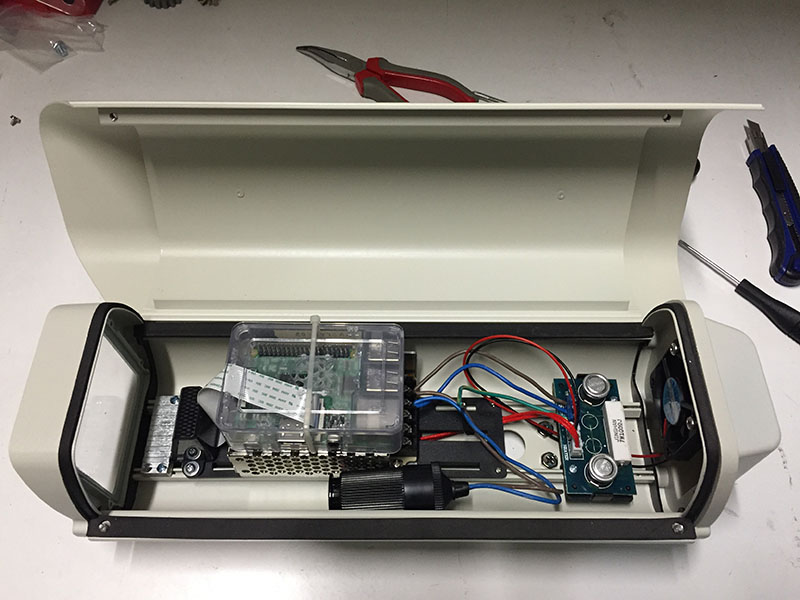
\includegraphics[width=\columnwidth]{camera_inside}
        \caption{Inside of a camera box}
	\end{subfigure} %
    \begin{subfigure}{0.48\columnwidth}
		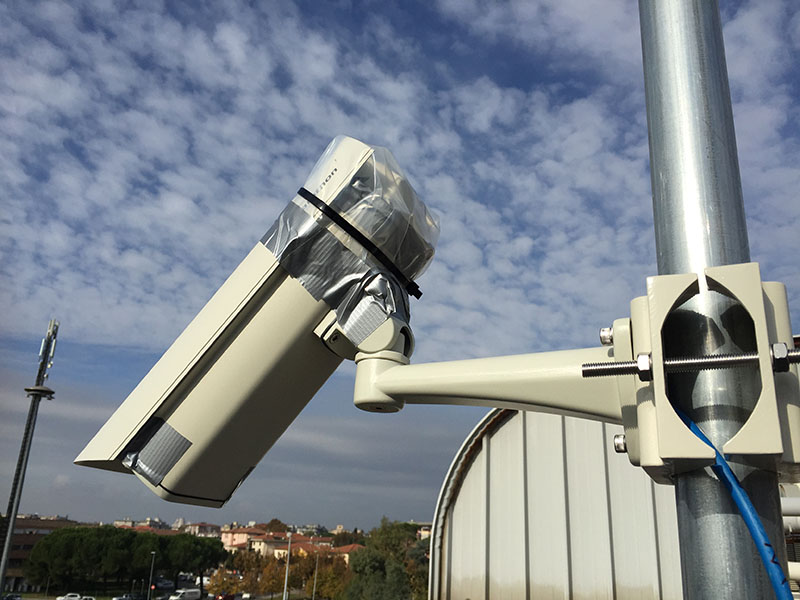
\includegraphics[width=\columnwidth]{camera_box}
        \caption{The complete camera box}
	\end{subfigure}

	\caption{Each Raspberry Pi is mounted inside a outdoor camera box (Figure $A$ on the left) and it is mounted on top of the roof of the building, attached to a steel pole (Figure $B$ on the right)}
	\label{fig:mini:camera-box}
\end{figure}

\begin{figure}
	\centering
		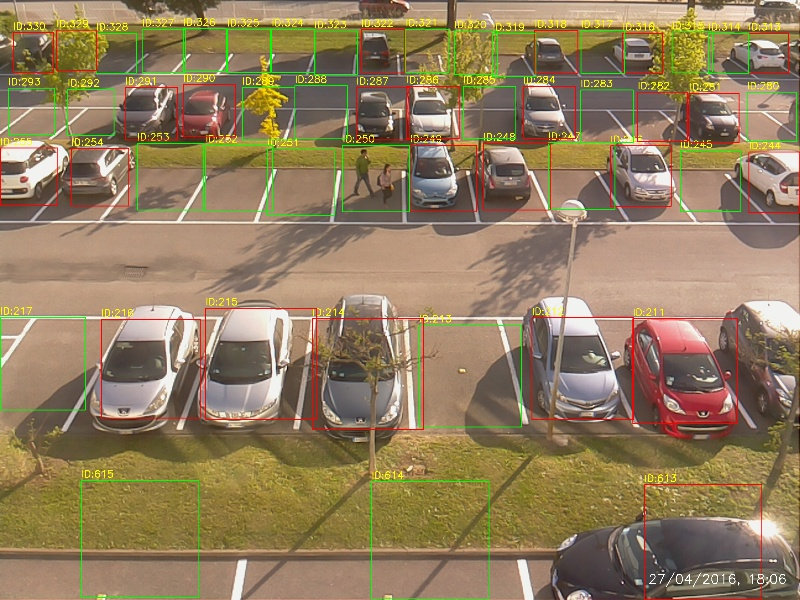
\includegraphics[width=\columnwidth,trim={0 0 0 3.5ex},clip]{detection-example}
        \caption{Example of classification of a portion of the parking lot}
	\label{fig:mini:detection-example}
\end{figure}

In this section, we describe the details of the deployment of a prototype of our proposed solution for parking lot visual occupancy detection in the campus of the National Research Council (CNR) in Pisa.

We deployed 9 smart cameras on the roof of the building in front of a section of the campus parking lot.
Each smart camera is built from a Rasbperry Pi 2 model B equipped with standard Raspberry Pi camera module and mounted on an outdoor camera box (see \ref{fig:mini:camera-box}).
The total cost for a single camera is roughly 80\euro.
Hardware and software details are briefly reported for completeness.
The smart cameras are equipped with an ARM Cortex-A7 CPU, 1GB RAM DDR2, and a 32GB micro SD card for storage.
The camera module is a 5MP fixed-focus camera that supports 1080p30, 720p60 and VGA90 video modes, as well as still captures.
The view angles of the camera are 53.50$^{\circ}$ horizontally and 41.41$^{\circ}$ vertically.
We capture still pictures at a full-sensor resolution of $2592 \times 1944$ pixels.
We used the OpenCV\footnote{http://opencv.org/} library to elaborate the frames acquired by the cameras, and Caffe \cite{jia2014caffe} to train and use neural networks.

Periodically, cameras capture an image of a portion of the parking lot, segment individual slots using manually defined masks, and determine the occupancy status for each slot using the \gls{cnn} trained off-line.
\ref{fig:mini:detection-example} shows an example of the occupancy detection performed by one camera in which common challenging aspects --- such as shadows, obstacles (trees or lamps) or even people occupying the parking slots --- are correctly managed.
In total, the cameras monitor 164 parking spaces organized in five rows, the first comprised by 18 parking spaces each, and the others by 35 parking slots each.
The number of parking slots monitored by each camera spans from 20 to more than 50, roughly, depending on the position of the parking slots with respect to the building on which cameras are mounted.
In fact, some cameras are dedicated to monitor most of the parking spaces closest to the building, while further spaces are monitored by multiple cameras.
We exploit the redundancy offered by multiple cameras to reduce the classification uncertainty when possible.
We combine the predictions of slots monitored by more than one camera by manually assigning weights to each (slot, camera) couple that represent the quality of the camera view for that particular slot.
As correct prediction for a slot, we take the one with highest weighted confidence.

The predicted occupancy status for each slot is submitted to a server for visualization and counting purposes.

% A key aspect of the proposed system is its decentralized approach
% and the delegation of the parking decision to the smart cameras
% themselves. This solution has the clear advantage of being scalable
% as it requires no additional elaboration on the server side. In a
% centralized solution images of the parking at high resolution (of
% about 3MB) should be sent to the server which would thus become a
% bottleneck and a single point of failure. Moreover, the network may
% be easily congested with increasing number of parking lots to be monitored.

\section{Conclusions}
\label{sec:mini:conclusions}

We proposed and evaluated a reduced \acrlong{cnn} architecture for image classification that enables smart vision applications in embedded devices.
In the scope of visual parking lot occupancy detection, we defined \emph{mAlexNet}, a reduced version of the famous \emph{AlexNet} classifier, which is obtained by pruning layers and reducing the number of parameters of the original architecture.
Experiments on public datasets shown that our proposed architecture outperforms state-of-the-art approaches for visual parking lot occupancy detection based on shallow models and hand-crafted features while requiring a computational budget suitable for embedded devices.
Specifically, our architecture exhibits very high accuracies even in presence of challenging light conditions variation, shadows, and partial occlusions.
Moreover, multi-dataset experiments shown that the architectural reduction does not introduce a performance degradation in real scenarios, and it produces only a slight acceptable degradation of the generalization capability, i.e.\ the ability of classifying images coming from different parking lots with different imaging conditions.

We tested our approach on a real scenario in the parking lot of the campus of the CNR Area in Pisa.
We deployed a decentralized system comprised by 9 smart cameras which monitors multiple slots and perform the occupancy detection for each slot on board.
The delegation of parking slot occupancy detection to smart cameras provides a twofold advantage.
First, with a cost of a single camera (roughly 80\euro), we are able to monitor at most 50 slots in our configuration, drastically reducing the cost per single slot that is nearly 100\euro for magnetic ground sensors while maintaining the same level of accuracy;
Second, the decentralized nature of our solution enables a higher degree of scalability, since there is no need of a central server to analyze images and a high bandwidth to transfer them.
In addition, the flexibility of the infrastructure does not limit the applications only to occupancy detection;
the spare computational resources can be used to perform other analyses such as video surveillance activities.

As a further contribution, we collected and made publicly available \emph{CNRPark-EXT}, a dataset containing images of a real parking lot taken by nine smart cameras, in different days, with different weather and light conditions.
\emph{CNRPark-EXT} covers a high variability of occlusions, point of views, light and weather conditions, which we experimentally demonstrated being of significant importance for the robustenss and generalization of occupancy detection systems.
This makes the dataset more compatible with real scenarios of outdoor parking lots, and represents a good complement to other publicly available datasets, for more reliable assessments.

%==========================

% Thanks to the use of deep CNN, the proposed solution is robust to disturbances created by partial occlusions, by the presence of shadows and by the variation of light conditions. % TODO integrate
% Moreover, it exhibits a good generalization property: in fact, the quality of the results is maintained when we consider parking lots and scenarios significantly different from the ones used during the CNN training phase.

%==========================

% \emph{mLeNet} is based on LeNet-5, proposed by \cite{lecun1998gradient}, having two convolutional layers followed by max pooling and two fully connected layers.
% The first layer (\emph{conv1}) is similar to the one proposed by \cite{krizhevsky2012imagenet} to be more suitable for a 224x224x3 input image.
% Layers \emph{conv2} and \emph{fc4} have a reduced number of filters and neurons with respect to \cite{lecun1998gradient} to better suit a binary classification task without overfitting.
% For \emph{fc5}, the last Gaussian RBF (radial basis function) layer is replaced with a classical inner product layer and a 2-way soft max classifier.

% Unlike \cite{krizhevsky2012imagenet} and \cite{lecun1998gradient}, both  architectures have a dense connection between convolutional layers.

% We used the Caffe framework \cite{jia2014caffe} to train the neural network and to initialize the classifier.

% We first compared the two proposed CNN architectures to select the one that offers the best performance.
% Afterwards, we compared our approach against other state-of-the-art methods.
% Finally, we performed experiments to analyze the difference between our CNN architecture.

% \subsection{Assessment of the Proposed CNNs}

% \noindent In order to assess the performance of the two CNN architectures
% \emph{mAlexNet} and \emph{mLeNet}, presented in Section
% \ref{sec:occupancy-detection}, we performed experiments using the
% \emph{CNRPark} dataset, considering two possible application
% scenarios:
% % a \emph{single camera scenario}, in which train and test data come from the same viewpoint, and
% % a \emph{multiple camera scenario}, in which training data and test data come from
% % different viewpoints.
% %
% \begin{inparaenum}[\itshape a\upshape)]
%   \item \emph{single camera scenario}, in which train and test data come from
%   the same viewpoint,
%   \item \emph{multiple camera scenario}, in which train data and
%   test data come from different viewpoints.
% \end{inparaenum}

% %Experiments are performed offline using the manually labeled data generated as
% %described in Subsection~\ref{sec:dataset}.
% Images of parking spaces are divided in two subsets,
% \emph{CNRPark A} and \emph{CNRPark B}, containing images respectively taken from
% a camera with central view and a camera with a side view of the parking lots
% (Figure~\ref{fig:cameraoverview}). Details are reported in
% Table~\ref{tbl:datasets}. All patches are shuffled and resized to a fixed size
% of 256x256 pixels. No information about the previous classification of a space
% is used to classify the same or other spaces, hence each image is classified
% independently from each other. For both the CNNs (mLeNet and mAlexNet), we
% perform a learning phase and a classification phase.

% For the single camera scenario, in order to limit problems of
% overfitting, we further divided the two subsets (\emph{CNRPark A}
% and \emph{CNRPark B}) considering independently odd numbered and
% even numbered spaces. Specifically, when we train on odd numbered
% we test on even numbered, and viceversa, for a total of eight
% experiments. This scenario allowed us to test the robustness of
% the proposed solution to possible changes that may occur during
% outdoor monitoring with fixed cameras, such as illumination
% changes, shadows and partial occlusions.

% For the multi camera scenario, we train both networks on an entire subset and
% then we test them on the other subset, for a total of four experiments. We tested
% the robustness of the proposed solution to viewpoint variations, allowing us to
% measure the ability of the solution to transfer the learned knowledge to a new
% unseen scenario.

% Training images are randomly cropped to 224x224 and randomly flipped
% horizontally, while for test images the central 224x224 crop is taken.
% We train our CNN models using the Caffe framework \cite{jia2014caffe} with
% gradient descend with momentum. The following hyper-parameters are used:
% momentum $0.9$; weight decay $5\cdot10^{-4}$. The initial learning rates are
% chosen independently for each experiment and they are reported in
% Table~\ref{tbl:cnn-experiments} (\emph{base lr} column). The learning rate is
% decreased two times by a factor 10 when the loss stabilizes, or after at most 10
% epochs, resulting in at most 30 epochs of training.
% Trained models are available for
% download.\footnote{http://claudiotest.isti.cnr.it/CNRPark/models/}

% \newcommand{\maxf}[1]{{\cellcolor[gray]{0.8}}#1}
% \begin{table}
%   \newcolumntype{Y}{>{\centering\arraybackslash}X}
%   \def\arraystretch{1.2}
%   \begin{tabularx}{\linewidth}{|Y|Y|Y|Y|Y|}
%     % \begin{tabular}{|c|c|c|c|c|}
%     % \hline
%     \multicolumn{5}{c}{\bfseries SINGLE CAMERA EXPERIMENTS} \\ \hline
%     \hline
%     \emph{train}            & \emph{test}             & \emph{net}    & \emph{base lr} & \emph{accuracy} \\ \hline
%     \multirow{2}{*}{A (even)} & \multirow{2}{*}{A (odd)}  & mLeNet          & 0.001            & 0.993             \\ \cline{3-5}
%                               &                           & \maxf{mAlexNet} & \maxf{0.01}      & \maxf{0.996}      \\ \hline
%     \multirow{2}{*}{A (odd)}  & \multirow{2}{*}{A (even)} & mLeNet          & 0.001            & 0.982             \\ \cline{3-5}
%                               &                           & \maxf{mAlexNet} & \maxf{0.005}     & \maxf{0.993}      \\ \hline
%     \multirow{2}{*}{B (even)} & \multirow{2}{*}{B (odd)}  & mLeNet          & 0.001            & 0.861             \\ \cline{3-5}
%                               &                           & \maxf{mAlexNet} & \maxf{0.01}      & \maxf{0.911}      \\ \hline
%     \multirow{2}{*}{B (odd)}  & \multirow{2}{*}{B (even)} & mLeNet          & 0.001            & 0.893             \\ \cline{3-5}
%                               &                           & \maxf{mAlexNet} & \maxf{0.005}     & \maxf{0.898}      \\ \hline
%   \end{tabularx}\\[2ex]
%   \begin{tabularx}{\linewidth}{|Y|Y|Y|Y|Y|}
%     % \hline
%     \multicolumn{5}{c}{\bfseries MULTI CAMERA EXPERIMENTS} \\ \hline
%     \hline
%     \emph{train}            & \emph{test}             & \emph{net}    & \emph{base lr} & \emph{accuracy} \\ \hline
%     \multirow{2}{*}{A}        & \multirow{2}{*}{B}        & mLeNet          & 0.0001           & 0.843             \\ \cline{3-5}
%                               &                           & \maxf{mAlexNet} & \maxf{0.001}     & \maxf{0.863}      \\ \hline
%     \multirow{2}{*}{B}        & \multirow{2}{*}{A}        & mLeNet          & 0.001            & 0.842             \\ \cline{3-5}
%                               &                           & \maxf{mAlexNet} & \maxf{0.0005}    & \maxf{0.907}      \\ \hline

%   \end{tabularx}
%   \vspace{1ex}
%   \caption{Settings and results of experiments performed on subsets $A$ and $B$
%   of \emph{CNRPark}, captured from different cameras. The even/odd
%   indication tells whether training or testing is performed only on images of
%   even or odd numbered spaces of that particular subset.}
%   \label{tbl:cnn-experiments}
% \end{table}

% \subsubsection{Results}

% \noindent The accuracy obtained at the end of the learning phase is reported
% in Table~\ref{tbl:cnn-experiments} for each configuration.

% Both CNNs, when tested in the single camera scenario, perform
% better on the subset \emph{CNRPark A}, which contains less
% occlusions and in which there are less variations between parking
% spaces. In fact, \emph{mAlexNet} reaches an accuracy of $0.996$
% in \emph{CNRPark A}. However, very good results are also obtained
% on subset \emph{CNRPark B}, where \emph{mAlexNet} reaches an
% accuracy of $0.911$, despite the very skewed viewpoint and the
% higher number of obstacles in the field of view. For the multi
% camera scenario, higher values of accuracy are obtained when
% training on the more complex subset \emph{CNRPark B}, from which
% the model can extract richer information and better generalize. In
% this case, \emph{mAlexNet} reaches an accuracy of $0.907$.

% In all configurations \emph{mAlexNet} offers the best
% performance, thanks to the use of a larger model that always
% boosts accuracy, although more effort is required to train it.


% \begin{figure*}[t]
%    \centering
%    \subfigure[]{\includegraphics[width=0.48\textwidth]{camera-a-output.jpg}}\qquad
%     \subfigure[]{\includegraphics[width=0.48\textwidth]{camera-b-output.jpg}}
%    \caption{\textsc{Output }}
%    \label{fig:output}
%\end{figure*}

% ===========

%\subsection{Multi-dataset experiments}

% We performed two types of comparative experiments using both
% \emph{CNRPark} and \emph{PKLot} datasets: \emph{intra-dataset}
% experiments and \emph{inter-dataset} experiments.

% With \emph{intra-dataset} experiments, we evaluated both
% techniques using, individually, one of the two dataset for both
% training and testing purposes. In this way, we estimated the
% performance of both techniques when the statistics of both train
% and test sets are similar.

% With \emph{inter-dataset} experiments, we used one of the two
% datasets to train and fine-tune each method, and we used the other
% dataset to test them. Hence, we estimated the ability of both
% techniques to generalize from the particular statistics of the
% training dataset.

% For more details about these experiments, see \cite{cnr.isti2015-TR-0402015}.


% For \emph{intra-dataset} experiments, both datasets have been
% divided into two partitions. \emph{CNRPark} has been divided in
% \emph{CNRParkEven}, containing images of even-numbered spaces,
% and \emph{CNRParkOdd}, containing images of odd-numbered spaces.\newline
% Both partitions have been used as training set and test set.
% \emph{PKLot} dataset has been divided in \emph{PKLot2Days} and
% \emph{PKLotNot2Days}. The former is formed choosing for each
% camera and for each weather condition the images of the first
% two days in chronological order, and the latter contains the
% remaining images. This partition strategy has been adopted to
% reduce training time, since only the smaller partition
% (\emph{PKLot2Days}) is used as training set.

% For \emph{inter-dataset} experiments, we trained on \emph{PKLot2Days} instead
% of using the whole \emph{PKLot} to reduce training times. Tests are however
% performed on the whole dataset.

% All the details of the datasets are reported in Table~\ref{tbl:datasets}, and
% results of performed experiments are summarized in
% Table~\ref{tbl:intra-inter-experiments}.

% In the \emph{intra-dataset} experiments, our method is
% comparable with the ones proposed in \cite{de2015pklot}.
% Using the highest confidence as classification output (having a
% threshold of $0.5$), the \emph{mAlexNet} achieves slightly higher
% accuracy values with respect to the other methods.

% In the \emph{inter-dataset} experiments, our method demonstrates
% a higher level of generalization, outperforming the other tested
% methods, achieving significantly higher accuracy values.

% \begin{table}
% 	\scriptsize
% 	\newcolumntype{Y}{>{\centering\arraybackslash}X}
% 	\newcolumntype{N}{S[table-format=1.2,round-mode=places,round-precision=2]}
% 	%\def\arraystretch{1.1}
% 	\begin{tabularx}{\linewidth}{|Y|N|N|N||N|N|}
% 		\multicolumn{4}{c}{\bfseries INTRA-DATASET} & \multicolumn{2}{c}{\bfseries INTER-DATASET}\\ \hline
% 		\textbf{train} & \multicolumn{1}{c|}{PKLot2Days}    & \multicolumn{1}{c|}{CNRParkOdd}  & \multicolumn{1}{c||}{CNRParkEven} & \multicolumn{1}{c|}{PKLot2Days} & \multicolumn{1}{c|}{CNRPark} \\
% 		\textbf{test}  & \multicolumn{1}{c|}{PKLotNot2Days} & \multicolumn{1}{c|}{CNRParkEven} & \multicolumn{1}{c||}{CNRParkOdd}  & \multicolumn{1}{c|}{CNRPark}    & \multicolumn{1}{c|}{PKLot}   \\ \cline{1-1}
% 		\textbf{model} &                                    &                                  &                                   &                                 &                              \\ \hline

% 		mAlex          & \maxf{0.981411554126166}           & \maxf{0.901312591152163}         & \maxf{0.907063776703571}          & \maxf{0.828830260648443}        & \maxf{0.903750400561001}     \\ \hline
% 		LPQu           & 0.965874918839068                  & 0.869227029654837                & 0.814907219709964                 & 0.646376350921806               & 0.398238824886945            \\ \hline
% 		LPQgd          & 0.970236471449698                  & 0.876519202722411                & 0.812880087322626                 & 0.617371265098538               & 0.409933050629474            \\ \hline
% 		LPQg           & 0.956938043299657                  & 0.868740884783666                & 0.816466552315609                 & 0.638350286077559               & 0.438087998402067            \\ \hline
% 		LBPuri         & 0.874336554245814                  & 0.850105331388754                & 0.763137377202557                 & 0.653051493960585               & 0.497392581394714            \\ \hline
% 		LBPu           & 0.950955664993196                  & 0.868416788202885                & 0.800249493216903                 & 0.642720915448188               & 0.466701346028662            \\ \hline
% 		LBPri          & 0.878793824909347                  & 0.864851725814293                & 0.819585217526899                 & 0.642005721551176               & 0.487172707533708            \\ \hline
% 		LBP            & 0.944891926341768                  & 0.874088478366553                & 0.872134726337128                 & 0.631277813095995               & 0.528790815908630            \\ \hline
% 	\end{tabularx}\\[5ex]

% 	\caption{Settings of \emph{intra-} and \emph{inter-dataset} experiments and achieved accuracy values.}
% 	\label{tbl:intra-inter-experiments}
% \end{table}

% For the comparisons, we evaluated the performance of the trained
% classifiers on the test sets measuring the accuracy and the Area
% Under the Curve (AUC) of Receiver Operating Characteristic (ROC)
% curves. ROC curves show how True Positive Rate (TPR), on y-axis,
% and False Positive Rate (FPR), on x-axis, vary as its score
% threshold is varied. AUC measures how much a curve leans near the
% perfect classification point, that is the point (0,1) on the ROC
% plot. AUC values range from 0 (perfect misclassification) to 1
% (perfect classification), where 0.5 indicates a classifier that
% performs like the random guessing classifier.

% \subsubsection{Results}

% In Figure~\ref{fig:roc-curves}, we report the ROC curves generated by
% each method tested on both datasets, and for convenience, in
% Table~\ref{tbl:intra-inter-experiments} we separately report the
% achieved accuracies.

% In the \emph{intra-dataset} experiments, our method is
% comparable with the ones proposed in \cite{de2015pklot} in terms
% of AUC. In fact, our \emph{mAlexNet} method reaches AUCs of
% $0.943$ on \emph{CNRParkEven}, $0.920$ on \emph{CNRParkOdd},
% and $0.996$ on \emph{PKLotNot2Days}, which are very close to
% respectively $0.957$, $0.923$, and $0.997$ of the best performing
% compared methods, as can be seen in Figure~\ref{fig:roc-curves}.

% Using the highest confidence as classification output (having a
% theshold of $0.5$), the \emph{mAlexNet} achieves slightly higher
% accuracy values with respect to the other methods. In fact, we reach
% and accuracy of $0.901$ on \emph{CNRParkEven}, $0.907$ on
% \emph{CNRParkOdd}, and $0.981$ on \emph{PKLotNot2Days}, which are
% higher than respectively $0.877$, $0.872$, and $0.970$ of the best
% performing compared methods, as can be seen in
% Table~\ref{tbl:intra-inter-experiments}.

% In the \emph{inter-dataset} experiments, our method demonstrates
% a higher level of generalization, outperforming the other tested
% methods. In fact, the \emph{mAlexNet} method reaches AUCs of
% $0.899$ on \emph{CNRPark}, and $0.989$ on \emph{PKLot}, which
% are definitively better than respectively $0.580$, and $0.743$, of
% the best performing compared methods, as can be seen still in
% Figure~\ref{fig:roc-curves}.

% Hence, the same situation goes for accuracy values when using $0.5$ as threshold,
% \emph{mAlexNet} achieves significantly higher accuracy values.
% In fact, as can be seen in Table~\ref{tbl:intra-inter-experiments},
% we reach and accuracy of $0.829$ on \emph{CNRPark}, and $0.904$
% on \emph{PKLot}, versus respectively $0.646$, and $0.529$, of
% the best performing compared methods.

% \usepackage{graphics} is needed for \includegraphics
% \begin{figure*}[htp]
%   \begin{center}
%     \begin{minipage}[t]{.495\textwidth}
%       \centering
%       \includegraphics[width=.9\linewidth]{eval/ROC-classify-CNRParkEven-train-on-CNRParkOdd}\\[3ex]
%       \includegraphics[width=.9\linewidth]{eval/ROC-classify-CNRParkOdd-train-on-CNRParkEven}\\[3ex]
%       \includegraphics[width=.9\linewidth]{eval/ROC-classify-PKLotNot2Days-train-on-PKLot2Days}
%     \end{minipage} \hfill
%     \begin{minipage}[t]{.495\textwidth}
%       \includegraphics[width=.9\linewidth]{eval/ROC-classify-CNRPark-train-on-PKLot2Days}\\[3ex]
%       \includegraphics[width=.95\linewidth]{eval/ROC-classify-PKLot-train-on-CNRPark}\\[3ex]
%       \caption{ROC curves for intra-dataset (left column) and inter-dataset
%       (right column) experiments, where the positive class is `busy'.
%       Methods in the legends are sorted by descending values of AUC.}
%       \label{fig:roc-curves}
%     \end{minipage}
%   \end{center}
% \end{figure*}


\cleardoublepage
\phantomsection
\addcontentsline{toc}{chapter}{\bibname}
\small
\bibliographystyle{plainnat}
\bibliography{thesis}

\end{document}
